% **************************************************************************************************************
% A Classic Thesis Style
% An Homage to The Elements of Typographic Style
%
% Copyright (C) 2018 André Miede and Ivo Pletikosić
%
% If you like the style then I would appreciate a postcard. My address
% can be found in the file ClassicThesis.pdf. A collection of the
% postcards I received so far is available online at
% http://postcards.miede.de
%
% License:
% This program is free software; you can redistribute it and/or modify
% it under the terms of the GNU General Public License as published by
% the Free Software Foundation; either version 2 of the License, or
% (at your option) any later version.
%
% This program is distributed in the hope that it will be useful,
% but WITHOUT ANY WARRANTY; without even the implied warranty of
% MERCHANTABILITY or FITNESS FOR A PARTICULAR PURPOSE.  See the
% GNU General Public License for more details.
%
% You should have received a copy of the GNU General Public License
% along with this program; see the file COPYING.  If not, write to
% the Free Software Foundation, Inc., 59 Temple Place - Suite 330,
% Boston, MA 02111-1307, USA.
%
% PLEASE SEE ALSO THE AUTHORS' NOTE REGARDING THIS LICENSE
% IN THE DOCUMENTATION (ClassicThesis.pdf --> Chapter 1 / Chapter01.tex)
% **************************************************************************************************************
\RequirePackage{silence} % :-\
    \WarningFilter{scrreprt}{Usage of package `titlesec'}
    % \WarningFilter{scrreprt}{Activating an ugly workaround}
    \WarningFilter{titlesec}{Non standard sectioning command detected}
    \documentclass[openany,%1headlines,
                headinclude,footinclude,abstract=on,
                BCOR=5mm,paper=a4,fontsize=12pt
                ]{scrreprt}


    %original
    %\documentclass[twoside,openright,titlepage,numbers=noenddot,%1headlines,
     %           headinclude,footinclude,cleardoublepage=empty,abstract=on,
      %          BCOR=5mm,paper=a4,fontsize=12pt
       %         ]{scrreprt}

%============ Modificación Español en Xelatex
\usepackage{polyglossia} 
\setmainlanguage[variant=mexican]{spanish}

% Adjuntar otros lenguajes utilizados en el documento
\setotherlanguage[variant=american]{english}
\setotherlanguage[variant=german]{german}
%============================================

%********************************************************************
% Note: Make all your adjustments in here
%*******************************************************
% ****************************************************************************************************
% classicthesis-config.tex
% formerly known as loadpackages.sty, classicthesis-ldpkg.sty, and classicthesis-preamble.sty
% Use it at the beginning of your ClassicThesis.tex, or as a LaTeX Preamble
% in your ClassicThesis.{tex,lyx} with % ****************************************************************************************************
% classicthesis-config.tex
% formerly known as loadpackages.sty, classicthesis-ldpkg.sty, and classicthesis-preamble.sty
% Use it at the beginning of your ClassicThesis.tex, or as a LaTeX Preamble
% in your ClassicThesis.{tex,lyx} with % ****************************************************************************************************
% classicthesis-config.tex
% formerly known as loadpackages.sty, classicthesis-ldpkg.sty, and classicthesis-preamble.sty
% Use it at the beginning of your ClassicThesis.tex, or as a LaTeX Preamble
% in your ClassicThesis.{tex,lyx} with \input{classicthesis-config}
% ****************************************************************************************************
% If you like the classicthesis, then I would appreciate a postcard.
% My address can be found in the file ClassicThesis.pdf. A collection
% of the postcards I received so far is available online at
% http://postcards.miede.de
% ****************************************************************************************************


% ****************************************************************************************************
% 0. Set the encoding of your files. UTF-8 is the only sensible encoding nowadays. If you can't read
% äöüßáéçèê∂åëæƒÏ€ then change the encoding setting in your editor, not the line below. If your editor
% does not support utf8 use another editor!
% ****************************************************************************************************


\PassOptionsToPackage{utf8}{inputenc}
  \usepackage{inputenc}

\PassOptionsToPackage{T1}{fontenc} % T2A for cyrillics
  \usepackage{fontenc}


% ****************************************************************************************************
% 1. Configure classicthesis for your needs here, e.g., remove "drafting" below
% in order to deactivate the time-stamp on the pages
% (see ClassicThesis.pdf for more information):
% ****************************************************************************************************
\PassOptionsToPackage{
  drafting=true,    % print version information on the bottom of the pages
  tocaligned=false, % the left column of the toc will be aligned (no indentation)
  dottedtoc=true,  % page numbers in ToC flushed right
  eulerchapternumbers=true, % use AMS Euler for chapter font (otherwise Palatino)
  linedheaders=false,       % chaper headers will have line above and beneath
  floatperchapter=true,     % numbering per chapter for all floats (i.e., Figure 1.1)
  eulermath=false,  % use awesome Euler fonts for mathematical formulae (only with pdfLaTeX)
  beramono=true,    % toggle a nice monospaced font (w/ bold)
  palatino=true,    % deactivate standard font for loading another one, see the last section at the end of this file for suggestions
  style=classicthesis % classicthesis, arsclassica
}{classicthesis}


% ****************************************************************************************************
% 2. Personal data and user ad-hoc commands (insert your own data here)
% ****************************************************************************************************
\newcommand{\myTitle}{ANN's como Propagadores en Dinámica Cuántica}
\newcommand{\mySubtitle}{Facultad de Ciencias}
\newcommand{\myDegree}{Física \xspace}
\newcommand{\myName}{Itzel Jessica Martínez Marcelo \xspace}
\newcommand{\myProf}{Put name here \xspace}
\newcommand{\myOtherProf}{Put name here\xspace}
\newcommand{\mySupervisor}{Dr. Huziel Enoc Sauceda Felix \xspace}
\newcommand{\myFaculty}{Facultad de Ciencias \xspace}
\newcommand{\myDepartment}{Put data here\xspace}
\newcommand{\myUni}{Universidad Nacional Autónoma de México \xspace}
\newcommand{\myLocation}{Ciudad de México, México\xspace}
\newcommand{\myTime}{2023 \xspace}
\newcommand{\myVersion}{\classicthesis}

% ********************************************************************
% Setup, finetuning, and useful commands
% ********************************************************************
\providecommand{\mLyX}{L\kern-.1667em\lower.25em\hbox{Y}\kern-.125emX\@}
\newcommand{\ie}{i.\,e.}
\newcommand{\Ie}{I.\,e.}
\newcommand{\eg}{e.\,g.}
\newcommand{\Eg}{E.\,g.}
% ****************************************************************************************************


% ****************************************************************************************************
% 3. Loading some handy packages
% ****************************************************************************************************
% ********************************************************************
% Packages with options that might require adjustments
% ********************************************************************
\PassOptionsToPackage{ngerman,american}{babel} % change this to your language(s), main language last
  \usepackage{babel}
% Spanish languages need extra options in order to work with this template
%\PassOptionsToPackage{spanish,es-lcroman}{babel}
%\PassOptionsToPackage{es-tabla,spanish,es-lcroman,english}{babel}

%####### Cambio de lenguaje
\PassOptionsToPackage{es-tabla,spanish,es-lcroman, english}{polyglossia}%,es-lcroman,english}{babel}
  \usepackage{polyglossia}
\gappto\captionsspanish{\renewcommand{\tablename}{Tabla}}


%#######

\usepackage{csquotes}
\PassOptionsToPackage{%
  %backend=biber,bibencoding=utf8, %instead of bibtex
  backend=bibtex8,bibencoding=ascii,%
  language=auto,%
  style=numeric-comp,%
  %style=authoryear-comp, % Author 1999, 2010
  %bibstyle=authoryear,dashed=false, % dashed: substitute rep. author with ---
  sorting=nyt, % name, year, title
  maxbibnames=10, % default: 3, et al.
  %backref=true,%
  natbib=true % natbib compatibility mode (\citep and \citet still work)
}{biblatex}
    \usepackage{biblatex}





%\PassOptionsToPackage{fleqn}{amsmath}       % math environments and more by the AMS --j: left align equation
  \usepackage{amsmath}

% ********************************************************************
% General useful packages
% ********************************************************************
\usepackage{graphicx} %
\usepackage{scrhack} % fix warnings when using KOMA with listings package
\usepackage{xspace} % to get the spacing after macros right
\PassOptionsToPackage{printonlyused,smaller}{acronym}
  \usepackage{acronym} % nice macros for handling all acronyms in the thesis
  %\renewcommand{\bflabel}[1]{{#1}\hfill} % fix the list of acronyms --> no longer working
  %\renewcommand*{\acsfont}[1]{\textsc{#1}}
  %\renewcommand*{\aclabelfont}[1]{\acsfont{#1}}
  %\def\bflabel#1{{#1\hfill}}
  \def\bflabel#1{{\acsfont{#1}\hfill}}
  \def\aclabelfont#1{\acsfont{#1}}
% ****************************************************************************************************
%\usepackage{pgfplots} % External TikZ/PGF support (thanks to Andreas Nautsch)
%\usetikzlibrary{external}
%\tikzexternalize[mode=list and make, prefix=ext-tikz/]
% ****************************************************************************************************


% ****************************************************************************************************
% 4. Setup floats: tables, (sub)figures, and captions
% ****************************************************************************************************
\usepackage{tabularx} % better tables
  \setlength{\extrarowheight}{3pt} % increase table row height
\newcommand{\tableheadline}[1]{\multicolumn{1}{l}{\spacedlowsmallcaps{#1}}}
\newcommand{\myfloatalign}{\centering} % to be used with each float for alignment
\usepackage{subfig}
% ****************************************************************************************************


% ****************************************************************************************************
% 5. Setup code listings
% ****************************************************************************************************
\usepackage{listings}
%\lstset{emph={trueIndex,root},emphstyle=\color{BlueViolet}}%\underbar} % for special keywords
\lstset{language=[LaTeX]Tex,%C++,
  morekeywords={PassOptionsToPackage,selectlanguage},
  keywordstyle=\color{RoyalBlue},%\bfseries,
  basicstyle=\small\ttfamily,
  %identifierstyle=\color{NavyBlue},
  commentstyle=\color{Green}\ttfamily,
  stringstyle=\rmfamily,
  numbers=none,%left,%
  numberstyle=\scriptsize,%\tiny
  stepnumber=5,
  numbersep=8pt,
  showstringspaces=false,
  breaklines=true,
  %frameround=ftff,
  %frame=single,
  belowcaptionskip=.75\baselineskip
  %frame=L
}
% ****************************************************************************************************




% ****************************************************************************************************
% 6. Last calls before the bar closes
% ****************************************************************************************************
% ********************************************************************
% Her Majesty herself
% ********************************************************************
\usepackage{classicthesis}


% ********************************************************************
% Fine-tune hyperreferences (hyperref should be called last)
% ********************************************************************
\hypersetup{%
  %draft, % hyperref's draft mode, for printing see below
  colorlinks=true, linktocpage=true, pdfstartpage=3, pdfstartview=FitV,%
  % uncomment the following line if you want to have black links (e.g., for printing)
  %colorlinks=false, linktocpage=false, pdfstartpage=3, pdfstartview=FitV, pdfborder={0 0 0},%
  breaklinks=true, pageanchor=true,%
  pdfpagemode=UseNone, %
  % pdfpagemode=UseOutlines,%
  plainpages=false, bookmarksnumbered, bookmarksopen=true, bookmarksopenlevel=1,%
  hypertexnames=true, pdfhighlight=/O,%nesting=true,%frenchlinks,%
  urlcolor=CTurl, linkcolor=CTlink, citecolor=CTcitation, %pagecolor=RoyalBlue,%
  %urlcolor=Black, linkcolor=Black, citecolor=Black, %pagecolor=Black,%
  pdftitle={\myTitle},%
  pdfauthor={\textcopyright\ \myName, \myUni, \myFaculty},%
  pdfsubject={},%
  pdfkeywords={},%
  pdfcreator={pdfLaTeX},%
  pdfproducer={LaTeX with hyperref and classicthesis}%
}


% ********************************************************************
% Setup autoreferences (hyperref and babel)
% ********************************************************************
% There are some issues regarding autorefnames
% http://www.tex.ac.uk/cgi-bin/texfaq2html?label=latexwords
% you have to redefine the macros for the
% language you use, e.g., american, ngerman
% (as chosen when loading babel/AtBeginDocument)
% ********************************************************************
\makeatletter
%\@ifpackageloaded{babel}%
\@ifpackageloaded{polyglossia}% xelatex
  {%
    %\addto\extrasamerican{% babel
    \appto{\blockextras@spanish}{% xelatex polyglossia
      %\renewcommand*{\sectionautorefname}{Section}%
      
      \renewcommand*{\figureautorefname}{Figura}%
      \renewcommand*{\tableautorefname}{Tabla}%
      \renewcommand*{\partautorefname}{Parte}%
      \renewcommand*{\chapterautorefname}{Capítulo}%
      \renewcommand*{\sectionautorefname}{\adfS}%
      \renewcommand*{\subsectionautorefname}{\adfS}%
      \renewcommand*{\subsubsectionautorefname}{\adfS}%
      \renewcommand*{\equationautorefname}{Ecuación}%
    }%
    %\addto\extrasngerman{% babel
    \appto{\blockextras@german}{% xelatex
      \renewcommand*{\paragraphautorefname}{Absatz}%
      \renewcommand*{\subparagraphautorefname}{Unterabsatz}%
      \renewcommand*{\footnoteautorefname}{Fu\"snote}%
      \renewcommand*{\FancyVerbLineautorefname}{Zeile}%
      \renewcommand*{\theoremautorefname}{Theorem}%
      \renewcommand*{\appendixautorefname}{Anhang}%
      \renewcommand*{\equationautorefname}{Gleichung}%
      \renewcommand*{\itemautorefname}{Punkt}%
    }%
      % Fix to getting autorefs for subfigures right (thanks to Belinda Vogt for changing the definition)
      \providecommand{\subfigureautorefname}{\figureautorefname}%
    }{\relax}
\makeatother


% ********************************************************************
% Development Stuff
% ********************************************************************
\listfiles
%\PassOptionsToPackage{l2tabu,orthodox,abort}{nag}
%  \usepackage{nag}
%\PassOptionsToPackage{warning, all}{onlyamsmath}
%  \usepackage{onlyamsmath}


% ****************************************************************************************************
% 7. Personalizado: fancy horizontal rules
% ****************************************************************************************************
\PassOptionsToPackage{svgnames}{xcolor}

\usepackage[object=vectorian]{pgfornament} %%  http://altermundus.com/pages/tkz/ornament/index.html
\usepackage{lipsum,tikz}

\newcommand{\sectionline}{%
  \noindent
  \begin{center}
  {\color{DarkViolet}
    \resizebox{0.5\linewidth}{1ex}
    {{%
    {\begin{tikzpicture}
    \node  (C) at (0,0) {};
    \node (D) at (9,0) {};
    \path (C) to [ornament=85] (D);
    \end{tikzpicture}}}}}%
    \end{center}
  }
%% A macro with two arguments to change ornaments and colors easily
%% Syntax -- \sectionlinetwo{<color>}{<ornament>}
\newcommand{\sectionlinetwo}[2]{%
  \nointerlineskip \vspace{.5\baselineskip}\hspace{\fill}
  {\color{CTsemi}
    \resizebox{0.5\linewidth}{2ex}
    {{%
    {\begin{tikzpicture}
    \node  (C) at (0,0) {};
    \node (D) at (9,0) {};
    \path (C) to [ornament=#2] (D);
    \end{tikzpicture}}}}}%
    \hspace{\fill}
    \par\nointerlineskip \vspace{.5\baselineskip}
  }

%% OJO modificar o mover esto:  % Titlesec for configuring the header
\usepackage{auto-pst-pdf} % Vectorian Ornaments XeTeX auxiliary (from: https://tex.stackexchange.com/questions/253477/how-to-use-psvectorian-with-pdflatex)
\usepackage{psvectorian} % Vectorian Ornaments

\let\clipbox\relax % PSTricks (used by PSVectorian) already defines a \clipbox, so we need this workaround
\usepackage{adjustbox} % Adjustbox to rescale the ornaments (scalebox breaks titlesec for some reason...)

\newcommand{\otherfancydraw}{% Defining a command to shorten things
\renewcommand*{\psvectorianDefaultColor}{CTsemi}%
\begin{adjustbox}{max height=0.5\baselineskip}% Rescaling to have height of 0.5\baselineskip
  \raisebox{-0.25\baselineskip}{
  \rotatebox[origin=c]{0}{% And rotating 90 degrees %fig: 7 (45 grad)
  \psvectorian{25}% Ornament n° 26 (http://melusine.eu.org/syracuse/pstricks/vectorian/psvectorian.pdf)
  }}%
\end{adjustbox}%
}

% A command to create a rule centered vertically on the text (from: https://tex.stackexchange.com/questions/15119/draw-horizontal-line-left-and-right-of-some-text-a-single-line/15122#15122)
\newcommand*\ruleline[1]{\par\noindent\raisebox{.8ex}{\makebox[\linewidth]{\hrulefill\hspace{1ex}\raisebox{-.8ex}{#1}\hspace{1ex}\hrulefill}}}




%********************************************************************
% Intento de fondo transparente. Imagen para portada
%********************************************************************
%\usepackage{transparent}
\usepackage{eso-pic}
\newcommand\BackgroundPic{%
\put(0,0){%
\parbox[b][\paperheight]{\paperwidth}{%
\vfill
\centering

\includegraphics[width=\paperwidth,height=\paperheight,%
keepaspectratio]{gfx/LOgo-UNAM.png}%
\vfill
}}}







% ********************************************************************
% Changing the text area
% ********************************************************************
%\areaset[current]{312pt}{761pt} % 686 (factor 2.2) + 33 head + 42 head \the\footskip
%\setlength{\marginparwidth}{5em}%
%\setlength{\marginparsep}{2em}%
% ********************************************************************
% Using different fonts
% ********************************************************************
%\usepackage[oldstylenums]{kpfonts} % oldstyle notextcomp
% \usepackage[osf]{libertine}
%\usepackage[light,condensed,math]{iwona}
%\renewcommand{\sfdefault}{iwona}
%\usepackage{lmodern} % <-- no osf support :-(
%\usepackage{cfr-lm} %
%\usepackage[urw-garamond]{mathdesign} <-- no osf support :-(
%\usepackage[default,osfigures]{opensans} % scale=0.95
%\usepackage[sfdefault]{FiraSans}
% \usepackage[opticals,mathlf]{MinionPro} % onlytext
% ********************************************************************
%\usepackage[largesc,osf]{newpxtext}
%\linespread{1.05} % a bit more for Palatino
% Used to fix these:
% https://bitbucket.org/amiede/classicthesis/issues/139/italics-in-pallatino-capitals-chapter
% https://bitbucket.org/amiede/classicthesis/issues/45/problema-testatine-su-classicthesis-style
% ********************************************************************
% ****************************************************************************************************

% ****************************************************************************************************
% If you like the classicthesis, then I would appreciate a postcard.
% My address can be found in the file ClassicThesis.pdf. A collection
% of the postcards I received so far is available online at
% http://postcards.miede.de
% ****************************************************************************************************


% ****************************************************************************************************
% 0. Set the encoding of your files. UTF-8 is the only sensible encoding nowadays. If you can't read
% äöüßáéçèê∂åëæƒÏ€ then change the encoding setting in your editor, not the line below. If your editor
% does not support utf8 use another editor!
% ****************************************************************************************************


\PassOptionsToPackage{utf8}{inputenc}
  \usepackage{inputenc}

\PassOptionsToPackage{T1}{fontenc} % T2A for cyrillics
  \usepackage{fontenc}


% ****************************************************************************************************
% 1. Configure classicthesis for your needs here, e.g., remove "drafting" below
% in order to deactivate the time-stamp on the pages
% (see ClassicThesis.pdf for more information):
% ****************************************************************************************************
\PassOptionsToPackage{
  drafting=true,    % print version information on the bottom of the pages
  tocaligned=false, % the left column of the toc will be aligned (no indentation)
  dottedtoc=true,  % page numbers in ToC flushed right
  eulerchapternumbers=true, % use AMS Euler for chapter font (otherwise Palatino)
  linedheaders=false,       % chaper headers will have line above and beneath
  floatperchapter=true,     % numbering per chapter for all floats (i.e., Figure 1.1)
  eulermath=false,  % use awesome Euler fonts for mathematical formulae (only with pdfLaTeX)
  beramono=true,    % toggle a nice monospaced font (w/ bold)
  palatino=true,    % deactivate standard font for loading another one, see the last section at the end of this file for suggestions
  style=classicthesis % classicthesis, arsclassica
}{classicthesis}


% ****************************************************************************************************
% 2. Personal data and user ad-hoc commands (insert your own data here)
% ****************************************************************************************************
\newcommand{\myTitle}{ANN's como Propagadores en Dinámica Cuántica}
\newcommand{\mySubtitle}{Facultad de Ciencias}
\newcommand{\myDegree}{Física \xspace}
\newcommand{\myName}{Itzel Jessica Martínez Marcelo \xspace}
\newcommand{\myProf}{Put name here \xspace}
\newcommand{\myOtherProf}{Put name here\xspace}
\newcommand{\mySupervisor}{Dr. Huziel Enoc Sauceda Felix \xspace}
\newcommand{\myFaculty}{Facultad de Ciencias \xspace}
\newcommand{\myDepartment}{Put data here\xspace}
\newcommand{\myUni}{Universidad Nacional Autónoma de México \xspace}
\newcommand{\myLocation}{Ciudad de México, México\xspace}
\newcommand{\myTime}{2023 \xspace}
\newcommand{\myVersion}{\classicthesis}

% ********************************************************************
% Setup, finetuning, and useful commands
% ********************************************************************
\providecommand{\mLyX}{L\kern-.1667em\lower.25em\hbox{Y}\kern-.125emX\@}
\newcommand{\ie}{i.\,e.}
\newcommand{\Ie}{I.\,e.}
\newcommand{\eg}{e.\,g.}
\newcommand{\Eg}{E.\,g.}
% ****************************************************************************************************


% ****************************************************************************************************
% 3. Loading some handy packages
% ****************************************************************************************************
% ********************************************************************
% Packages with options that might require adjustments
% ********************************************************************
\PassOptionsToPackage{ngerman,american}{babel} % change this to your language(s), main language last
  \usepackage{babel}
% Spanish languages need extra options in order to work with this template
%\PassOptionsToPackage{spanish,es-lcroman}{babel}
%\PassOptionsToPackage{es-tabla,spanish,es-lcroman,english}{babel}

%####### Cambio de lenguaje
\PassOptionsToPackage{es-tabla,spanish,es-lcroman, english}{polyglossia}%,es-lcroman,english}{babel}
  \usepackage{polyglossia}
\gappto\captionsspanish{\renewcommand{\tablename}{Tabla}}


%#######

\usepackage{csquotes}
\PassOptionsToPackage{%
  %backend=biber,bibencoding=utf8, %instead of bibtex
  backend=bibtex8,bibencoding=ascii,%
  language=auto,%
  style=numeric-comp,%
  %style=authoryear-comp, % Author 1999, 2010
  %bibstyle=authoryear,dashed=false, % dashed: substitute rep. author with ---
  sorting=nyt, % name, year, title
  maxbibnames=10, % default: 3, et al.
  %backref=true,%
  natbib=true % natbib compatibility mode (\citep and \citet still work)
}{biblatex}
    \usepackage{biblatex}





%\PassOptionsToPackage{fleqn}{amsmath}       % math environments and more by the AMS --j: left align equation
  \usepackage{amsmath}

% ********************************************************************
% General useful packages
% ********************************************************************
\usepackage{graphicx} %
\usepackage{scrhack} % fix warnings when using KOMA with listings package
\usepackage{xspace} % to get the spacing after macros right
\PassOptionsToPackage{printonlyused,smaller}{acronym}
  \usepackage{acronym} % nice macros for handling all acronyms in the thesis
  %\renewcommand{\bflabel}[1]{{#1}\hfill} % fix the list of acronyms --> no longer working
  %\renewcommand*{\acsfont}[1]{\textsc{#1}}
  %\renewcommand*{\aclabelfont}[1]{\acsfont{#1}}
  %\def\bflabel#1{{#1\hfill}}
  \def\bflabel#1{{\acsfont{#1}\hfill}}
  \def\aclabelfont#1{\acsfont{#1}}
% ****************************************************************************************************
%\usepackage{pgfplots} % External TikZ/PGF support (thanks to Andreas Nautsch)
%\usetikzlibrary{external}
%\tikzexternalize[mode=list and make, prefix=ext-tikz/]
% ****************************************************************************************************


% ****************************************************************************************************
% 4. Setup floats: tables, (sub)figures, and captions
% ****************************************************************************************************
\usepackage{tabularx} % better tables
  \setlength{\extrarowheight}{3pt} % increase table row height
\newcommand{\tableheadline}[1]{\multicolumn{1}{l}{\spacedlowsmallcaps{#1}}}
\newcommand{\myfloatalign}{\centering} % to be used with each float for alignment
\usepackage{subfig}
% ****************************************************************************************************


% ****************************************************************************************************
% 5. Setup code listings
% ****************************************************************************************************
\usepackage{listings}
%\lstset{emph={trueIndex,root},emphstyle=\color{BlueViolet}}%\underbar} % for special keywords
\lstset{language=[LaTeX]Tex,%C++,
  morekeywords={PassOptionsToPackage,selectlanguage},
  keywordstyle=\color{RoyalBlue},%\bfseries,
  basicstyle=\small\ttfamily,
  %identifierstyle=\color{NavyBlue},
  commentstyle=\color{Green}\ttfamily,
  stringstyle=\rmfamily,
  numbers=none,%left,%
  numberstyle=\scriptsize,%\tiny
  stepnumber=5,
  numbersep=8pt,
  showstringspaces=false,
  breaklines=true,
  %frameround=ftff,
  %frame=single,
  belowcaptionskip=.75\baselineskip
  %frame=L
}
% ****************************************************************************************************




% ****************************************************************************************************
% 6. Last calls before the bar closes
% ****************************************************************************************************
% ********************************************************************
% Her Majesty herself
% ********************************************************************
\usepackage{classicthesis}


% ********************************************************************
% Fine-tune hyperreferences (hyperref should be called last)
% ********************************************************************
\hypersetup{%
  %draft, % hyperref's draft mode, for printing see below
  colorlinks=true, linktocpage=true, pdfstartpage=3, pdfstartview=FitV,%
  % uncomment the following line if you want to have black links (e.g., for printing)
  %colorlinks=false, linktocpage=false, pdfstartpage=3, pdfstartview=FitV, pdfborder={0 0 0},%
  breaklinks=true, pageanchor=true,%
  pdfpagemode=UseNone, %
  % pdfpagemode=UseOutlines,%
  plainpages=false, bookmarksnumbered, bookmarksopen=true, bookmarksopenlevel=1,%
  hypertexnames=true, pdfhighlight=/O,%nesting=true,%frenchlinks,%
  urlcolor=CTurl, linkcolor=CTlink, citecolor=CTcitation, %pagecolor=RoyalBlue,%
  %urlcolor=Black, linkcolor=Black, citecolor=Black, %pagecolor=Black,%
  pdftitle={\myTitle},%
  pdfauthor={\textcopyright\ \myName, \myUni, \myFaculty},%
  pdfsubject={},%
  pdfkeywords={},%
  pdfcreator={pdfLaTeX},%
  pdfproducer={LaTeX with hyperref and classicthesis}%
}


% ********************************************************************
% Setup autoreferences (hyperref and babel)
% ********************************************************************
% There are some issues regarding autorefnames
% http://www.tex.ac.uk/cgi-bin/texfaq2html?label=latexwords
% you have to redefine the macros for the
% language you use, e.g., american, ngerman
% (as chosen when loading babel/AtBeginDocument)
% ********************************************************************
\makeatletter
%\@ifpackageloaded{babel}%
\@ifpackageloaded{polyglossia}% xelatex
  {%
    %\addto\extrasamerican{% babel
    \appto{\blockextras@spanish}{% xelatex polyglossia
      %\renewcommand*{\sectionautorefname}{Section}%
      
      \renewcommand*{\figureautorefname}{Figura}%
      \renewcommand*{\tableautorefname}{Tabla}%
      \renewcommand*{\partautorefname}{Parte}%
      \renewcommand*{\chapterautorefname}{Capítulo}%
      \renewcommand*{\sectionautorefname}{\adfS}%
      \renewcommand*{\subsectionautorefname}{\adfS}%
      \renewcommand*{\subsubsectionautorefname}{\adfS}%
      \renewcommand*{\equationautorefname}{Ecuación}%
    }%
    %\addto\extrasngerman{% babel
    \appto{\blockextras@german}{% xelatex
      \renewcommand*{\paragraphautorefname}{Absatz}%
      \renewcommand*{\subparagraphautorefname}{Unterabsatz}%
      \renewcommand*{\footnoteautorefname}{Fu\"snote}%
      \renewcommand*{\FancyVerbLineautorefname}{Zeile}%
      \renewcommand*{\theoremautorefname}{Theorem}%
      \renewcommand*{\appendixautorefname}{Anhang}%
      \renewcommand*{\equationautorefname}{Gleichung}%
      \renewcommand*{\itemautorefname}{Punkt}%
    }%
      % Fix to getting autorefs for subfigures right (thanks to Belinda Vogt for changing the definition)
      \providecommand{\subfigureautorefname}{\figureautorefname}%
    }{\relax}
\makeatother


% ********************************************************************
% Development Stuff
% ********************************************************************
\listfiles
%\PassOptionsToPackage{l2tabu,orthodox,abort}{nag}
%  \usepackage{nag}
%\PassOptionsToPackage{warning, all}{onlyamsmath}
%  \usepackage{onlyamsmath}


% ****************************************************************************************************
% 7. Personalizado: fancy horizontal rules
% ****************************************************************************************************
\PassOptionsToPackage{svgnames}{xcolor}

\usepackage[object=vectorian]{pgfornament} %%  http://altermundus.com/pages/tkz/ornament/index.html
\usepackage{lipsum,tikz}

\newcommand{\sectionline}{%
  \noindent
  \begin{center}
  {\color{DarkViolet}
    \resizebox{0.5\linewidth}{1ex}
    {{%
    {\begin{tikzpicture}
    \node  (C) at (0,0) {};
    \node (D) at (9,0) {};
    \path (C) to [ornament=85] (D);
    \end{tikzpicture}}}}}%
    \end{center}
  }
%% A macro with two arguments to change ornaments and colors easily
%% Syntax -- \sectionlinetwo{<color>}{<ornament>}
\newcommand{\sectionlinetwo}[2]{%
  \nointerlineskip \vspace{.5\baselineskip}\hspace{\fill}
  {\color{CTsemi}
    \resizebox{0.5\linewidth}{2ex}
    {{%
    {\begin{tikzpicture}
    \node  (C) at (0,0) {};
    \node (D) at (9,0) {};
    \path (C) to [ornament=#2] (D);
    \end{tikzpicture}}}}}%
    \hspace{\fill}
    \par\nointerlineskip \vspace{.5\baselineskip}
  }

%% OJO modificar o mover esto:  % Titlesec for configuring the header
\usepackage{auto-pst-pdf} % Vectorian Ornaments XeTeX auxiliary (from: https://tex.stackexchange.com/questions/253477/how-to-use-psvectorian-with-pdflatex)
\usepackage{psvectorian} % Vectorian Ornaments

\let\clipbox\relax % PSTricks (used by PSVectorian) already defines a \clipbox, so we need this workaround
\usepackage{adjustbox} % Adjustbox to rescale the ornaments (scalebox breaks titlesec for some reason...)

\newcommand{\otherfancydraw}{% Defining a command to shorten things
\renewcommand*{\psvectorianDefaultColor}{CTsemi}%
\begin{adjustbox}{max height=0.5\baselineskip}% Rescaling to have height of 0.5\baselineskip
  \raisebox{-0.25\baselineskip}{
  \rotatebox[origin=c]{0}{% And rotating 90 degrees %fig: 7 (45 grad)
  \psvectorian{25}% Ornament n° 26 (http://melusine.eu.org/syracuse/pstricks/vectorian/psvectorian.pdf)
  }}%
\end{adjustbox}%
}

% A command to create a rule centered vertically on the text (from: https://tex.stackexchange.com/questions/15119/draw-horizontal-line-left-and-right-of-some-text-a-single-line/15122#15122)
\newcommand*\ruleline[1]{\par\noindent\raisebox{.8ex}{\makebox[\linewidth]{\hrulefill\hspace{1ex}\raisebox{-.8ex}{#1}\hspace{1ex}\hrulefill}}}




%********************************************************************
% Intento de fondo transparente. Imagen para portada
%********************************************************************
%\usepackage{transparent}
\usepackage{eso-pic}
\newcommand\BackgroundPic{%
\put(0,0){%
\parbox[b][\paperheight]{\paperwidth}{%
\vfill
\centering

\includegraphics[width=\paperwidth,height=\paperheight,%
keepaspectratio]{gfx/LOgo-UNAM.png}%
\vfill
}}}







% ********************************************************************
% Changing the text area
% ********************************************************************
%\areaset[current]{312pt}{761pt} % 686 (factor 2.2) + 33 head + 42 head \the\footskip
%\setlength{\marginparwidth}{5em}%
%\setlength{\marginparsep}{2em}%
% ********************************************************************
% Using different fonts
% ********************************************************************
%\usepackage[oldstylenums]{kpfonts} % oldstyle notextcomp
% \usepackage[osf]{libertine}
%\usepackage[light,condensed,math]{iwona}
%\renewcommand{\sfdefault}{iwona}
%\usepackage{lmodern} % <-- no osf support :-(
%\usepackage{cfr-lm} %
%\usepackage[urw-garamond]{mathdesign} <-- no osf support :-(
%\usepackage[default,osfigures]{opensans} % scale=0.95
%\usepackage[sfdefault]{FiraSans}
% \usepackage[opticals,mathlf]{MinionPro} % onlytext
% ********************************************************************
%\usepackage[largesc,osf]{newpxtext}
%\linespread{1.05} % a bit more for Palatino
% Used to fix these:
% https://bitbucket.org/amiede/classicthesis/issues/139/italics-in-pallatino-capitals-chapter
% https://bitbucket.org/amiede/classicthesis/issues/45/problema-testatine-su-classicthesis-style
% ********************************************************************
% ****************************************************************************************************

% ****************************************************************************************************
% If you like the classicthesis, then I would appreciate a postcard.
% My address can be found in the file ClassicThesis.pdf. A collection
% of the postcards I received so far is available online at
% http://postcards.miede.de
% ****************************************************************************************************


% ****************************************************************************************************
% 0. Set the encoding of your files. UTF-8 is the only sensible encoding nowadays. If you can't read
% äöüßáéçèê∂åëæƒÏ€ then change the encoding setting in your editor, not the line below. If your editor
% does not support utf8 use another editor!
% ****************************************************************************************************


\PassOptionsToPackage{utf8}{inputenc}
  \usepackage{inputenc}

\PassOptionsToPackage{T1}{fontenc} % T2A for cyrillics
  \usepackage{fontenc}


% ****************************************************************************************************
% 1. Configure classicthesis for your needs here, e.g., remove "drafting" below
% in order to deactivate the time-stamp on the pages
% (see ClassicThesis.pdf for more information):
% ****************************************************************************************************
\PassOptionsToPackage{
  drafting=true,    % print version information on the bottom of the pages
  tocaligned=false, % the left column of the toc will be aligned (no indentation)
  dottedtoc=true,  % page numbers in ToC flushed right
  eulerchapternumbers=true, % use AMS Euler for chapter font (otherwise Palatino)
  linedheaders=false,       % chaper headers will have line above and beneath
  floatperchapter=true,     % numbering per chapter for all floats (i.e., Figure 1.1)
  eulermath=false,  % use awesome Euler fonts for mathematical formulae (only with pdfLaTeX)
  beramono=true,    % toggle a nice monospaced font (w/ bold)
  palatino=true,    % deactivate standard font for loading another one, see the last section at the end of this file for suggestions
  style=classicthesis % classicthesis, arsclassica
}{classicthesis}


% ****************************************************************************************************
% 2. Personal data and user ad-hoc commands (insert your own data here)
% ****************************************************************************************************
\newcommand{\myTitle}{ANN's como Propagadores en Dinámica Cuántica}
\newcommand{\mySubtitle}{Facultad de Ciencias}
\newcommand{\myDegree}{Física \xspace}
\newcommand{\myName}{Itzel Jessica Martínez Marcelo \xspace}
\newcommand{\myProf}{Put name here \xspace}
\newcommand{\myOtherProf}{Put name here\xspace}
\newcommand{\mySupervisor}{Dr. Huziel Enoc Sauceda Felix \xspace}
\newcommand{\myFaculty}{Facultad de Ciencias \xspace}
\newcommand{\myDepartment}{Put data here\xspace}
\newcommand{\myUni}{Universidad Nacional Autónoma de México \xspace}
\newcommand{\myLocation}{Ciudad de México, México\xspace}
\newcommand{\myTime}{2023 \xspace}
\newcommand{\myVersion}{\classicthesis}

% ********************************************************************
% Setup, finetuning, and useful commands
% ********************************************************************
\providecommand{\mLyX}{L\kern-.1667em\lower.25em\hbox{Y}\kern-.125emX\@}
\newcommand{\ie}{i.\,e.}
\newcommand{\Ie}{I.\,e.}
\newcommand{\eg}{e.\,g.}
\newcommand{\Eg}{E.\,g.}
% ****************************************************************************************************


% ****************************************************************************************************
% 3. Loading some handy packages
% ****************************************************************************************************
% ********************************************************************
% Packages with options that might require adjustments
% ********************************************************************
\PassOptionsToPackage{ngerman,american}{babel} % change this to your language(s), main language last
  \usepackage{babel}
% Spanish languages need extra options in order to work with this template
%\PassOptionsToPackage{spanish,es-lcroman}{babel}
%\PassOptionsToPackage{es-tabla,spanish,es-lcroman,english}{babel}

%####### Cambio de lenguaje
\PassOptionsToPackage{es-tabla,spanish,es-lcroman, english}{polyglossia}%,es-lcroman,english}{babel}
  \usepackage{polyglossia}
\gappto\captionsspanish{\renewcommand{\tablename}{Tabla}}


%#######

\usepackage{csquotes}
\PassOptionsToPackage{%
  %backend=biber,bibencoding=utf8, %instead of bibtex
  backend=bibtex8,bibencoding=ascii,%
  language=auto,%
  style=numeric-comp,%
  %style=authoryear-comp, % Author 1999, 2010
  %bibstyle=authoryear,dashed=false, % dashed: substitute rep. author with ---
  sorting=nyt, % name, year, title
  maxbibnames=10, % default: 3, et al.
  %backref=true,%
  natbib=true % natbib compatibility mode (\citep and \citet still work)
}{biblatex}
    \usepackage{biblatex}





%\PassOptionsToPackage{fleqn}{amsmath}       % math environments and more by the AMS --j: left align equation
  \usepackage{amsmath}

% ********************************************************************
% General useful packages
% ********************************************************************
\usepackage{graphicx} %
\usepackage{scrhack} % fix warnings when using KOMA with listings package
\usepackage{xspace} % to get the spacing after macros right
\PassOptionsToPackage{printonlyused,smaller}{acronym}
  \usepackage{acronym} % nice macros for handling all acronyms in the thesis
  %\renewcommand{\bflabel}[1]{{#1}\hfill} % fix the list of acronyms --> no longer working
  %\renewcommand*{\acsfont}[1]{\textsc{#1}}
  %\renewcommand*{\aclabelfont}[1]{\acsfont{#1}}
  %\def\bflabel#1{{#1\hfill}}
  \def\bflabel#1{{\acsfont{#1}\hfill}}
  \def\aclabelfont#1{\acsfont{#1}}
% ****************************************************************************************************
%\usepackage{pgfplots} % External TikZ/PGF support (thanks to Andreas Nautsch)
%\usetikzlibrary{external}
%\tikzexternalize[mode=list and make, prefix=ext-tikz/]
% ****************************************************************************************************


% ****************************************************************************************************
% 4. Setup floats: tables, (sub)figures, and captions
% ****************************************************************************************************
\usepackage{tabularx} % better tables
  \setlength{\extrarowheight}{3pt} % increase table row height
\newcommand{\tableheadline}[1]{\multicolumn{1}{l}{\spacedlowsmallcaps{#1}}}
\newcommand{\myfloatalign}{\centering} % to be used with each float for alignment
\usepackage{subfig}
% ****************************************************************************************************


% ****************************************************************************************************
% 5. Setup code listings
% ****************************************************************************************************
\usepackage{listings}
%\lstset{emph={trueIndex,root},emphstyle=\color{BlueViolet}}%\underbar} % for special keywords
\lstset{language=[LaTeX]Tex,%C++,
  morekeywords={PassOptionsToPackage,selectlanguage},
  keywordstyle=\color{RoyalBlue},%\bfseries,
  basicstyle=\small\ttfamily,
  %identifierstyle=\color{NavyBlue},
  commentstyle=\color{Green}\ttfamily,
  stringstyle=\rmfamily,
  numbers=none,%left,%
  numberstyle=\scriptsize,%\tiny
  stepnumber=5,
  numbersep=8pt,
  showstringspaces=false,
  breaklines=true,
  %frameround=ftff,
  %frame=single,
  belowcaptionskip=.75\baselineskip
  %frame=L
}
% ****************************************************************************************************




% ****************************************************************************************************
% 6. Last calls before the bar closes
% ****************************************************************************************************
% ********************************************************************
% Her Majesty herself
% ********************************************************************
\usepackage{classicthesis}


% ********************************************************************
% Fine-tune hyperreferences (hyperref should be called last)
% ********************************************************************
\hypersetup{%
  %draft, % hyperref's draft mode, for printing see below
  colorlinks=true, linktocpage=true, pdfstartpage=3, pdfstartview=FitV,%
  % uncomment the following line if you want to have black links (e.g., for printing)
  %colorlinks=false, linktocpage=false, pdfstartpage=3, pdfstartview=FitV, pdfborder={0 0 0},%
  breaklinks=true, pageanchor=true,%
  pdfpagemode=UseNone, %
  % pdfpagemode=UseOutlines,%
  plainpages=false, bookmarksnumbered, bookmarksopen=true, bookmarksopenlevel=1,%
  hypertexnames=true, pdfhighlight=/O,%nesting=true,%frenchlinks,%
  urlcolor=CTurl, linkcolor=CTlink, citecolor=CTcitation, %pagecolor=RoyalBlue,%
  %urlcolor=Black, linkcolor=Black, citecolor=Black, %pagecolor=Black,%
  pdftitle={\myTitle},%
  pdfauthor={\textcopyright\ \myName, \myUni, \myFaculty},%
  pdfsubject={},%
  pdfkeywords={},%
  pdfcreator={pdfLaTeX},%
  pdfproducer={LaTeX with hyperref and classicthesis}%
}


% ********************************************************************
% Setup autoreferences (hyperref and babel)
% ********************************************************************
% There are some issues regarding autorefnames
% http://www.tex.ac.uk/cgi-bin/texfaq2html?label=latexwords
% you have to redefine the macros for the
% language you use, e.g., american, ngerman
% (as chosen when loading babel/AtBeginDocument)
% ********************************************************************
\makeatletter
%\@ifpackageloaded{babel}%
\@ifpackageloaded{polyglossia}% xelatex
  {%
    %\addto\extrasamerican{% babel
    \appto{\blockextras@spanish}{% xelatex polyglossia
      %\renewcommand*{\sectionautorefname}{Section}%
      
      \renewcommand*{\figureautorefname}{Figura}%
      \renewcommand*{\tableautorefname}{Tabla}%
      \renewcommand*{\partautorefname}{Parte}%
      \renewcommand*{\chapterautorefname}{Capítulo}%
      \renewcommand*{\sectionautorefname}{\adfS}%
      \renewcommand*{\subsectionautorefname}{\adfS}%
      \renewcommand*{\subsubsectionautorefname}{\adfS}%
      \renewcommand*{\equationautorefname}{Ecuación}%
    }%
    %\addto\extrasngerman{% babel
    \appto{\blockextras@german}{% xelatex
      \renewcommand*{\paragraphautorefname}{Absatz}%
      \renewcommand*{\subparagraphautorefname}{Unterabsatz}%
      \renewcommand*{\footnoteautorefname}{Fu\"snote}%
      \renewcommand*{\FancyVerbLineautorefname}{Zeile}%
      \renewcommand*{\theoremautorefname}{Theorem}%
      \renewcommand*{\appendixautorefname}{Anhang}%
      \renewcommand*{\equationautorefname}{Gleichung}%
      \renewcommand*{\itemautorefname}{Punkt}%
    }%
      % Fix to getting autorefs for subfigures right (thanks to Belinda Vogt for changing the definition)
      \providecommand{\subfigureautorefname}{\figureautorefname}%
    }{\relax}
\makeatother


% ********************************************************************
% Development Stuff
% ********************************************************************
\listfiles
%\PassOptionsToPackage{l2tabu,orthodox,abort}{nag}
%  \usepackage{nag}
%\PassOptionsToPackage{warning, all}{onlyamsmath}
%  \usepackage{onlyamsmath}


% ****************************************************************************************************
% 7. Personalizado: fancy horizontal rules
% ****************************************************************************************************
\PassOptionsToPackage{svgnames}{xcolor}

\usepackage[object=vectorian]{pgfornament} %%  http://altermundus.com/pages/tkz/ornament/index.html
\usepackage{lipsum,tikz}

\newcommand{\sectionline}{%
  \noindent
  \begin{center}
  {\color{DarkViolet}
    \resizebox{0.5\linewidth}{1ex}
    {{%
    {\begin{tikzpicture}
    \node  (C) at (0,0) {};
    \node (D) at (9,0) {};
    \path (C) to [ornament=85] (D);
    \end{tikzpicture}}}}}%
    \end{center}
  }
%% A macro with two arguments to change ornaments and colors easily
%% Syntax -- \sectionlinetwo{<color>}{<ornament>}
\newcommand{\sectionlinetwo}[2]{%
  \nointerlineskip \vspace{.5\baselineskip}\hspace{\fill}
  {\color{CTsemi}
    \resizebox{0.5\linewidth}{2ex}
    {{%
    {\begin{tikzpicture}
    \node  (C) at (0,0) {};
    \node (D) at (9,0) {};
    \path (C) to [ornament=#2] (D);
    \end{tikzpicture}}}}}%
    \hspace{\fill}
    \par\nointerlineskip \vspace{.5\baselineskip}
  }

%% OJO modificar o mover esto:  % Titlesec for configuring the header
\usepackage{auto-pst-pdf} % Vectorian Ornaments XeTeX auxiliary (from: https://tex.stackexchange.com/questions/253477/how-to-use-psvectorian-with-pdflatex)
\usepackage{psvectorian} % Vectorian Ornaments

\let\clipbox\relax % PSTricks (used by PSVectorian) already defines a \clipbox, so we need this workaround
\usepackage{adjustbox} % Adjustbox to rescale the ornaments (scalebox breaks titlesec for some reason...)

\newcommand{\otherfancydraw}{% Defining a command to shorten things
\renewcommand*{\psvectorianDefaultColor}{CTsemi}%
\begin{adjustbox}{max height=0.5\baselineskip}% Rescaling to have height of 0.5\baselineskip
  \raisebox{-0.25\baselineskip}{
  \rotatebox[origin=c]{0}{% And rotating 90 degrees %fig: 7 (45 grad)
  \psvectorian{25}% Ornament n° 26 (http://melusine.eu.org/syracuse/pstricks/vectorian/psvectorian.pdf)
  }}%
\end{adjustbox}%
}

% A command to create a rule centered vertically on the text (from: https://tex.stackexchange.com/questions/15119/draw-horizontal-line-left-and-right-of-some-text-a-single-line/15122#15122)
\newcommand*\ruleline[1]{\par\noindent\raisebox{.8ex}{\makebox[\linewidth]{\hrulefill\hspace{1ex}\raisebox{-.8ex}{#1}\hspace{1ex}\hrulefill}}}




%********************************************************************
% Intento de fondo transparente. Imagen para portada
%********************************************************************
%\usepackage{transparent}
\usepackage{eso-pic}
\newcommand\BackgroundPic{%
\put(0,0){%
\parbox[b][\paperheight]{\paperwidth}{%
\vfill
\centering

\includegraphics[width=\paperwidth,height=\paperheight,%
keepaspectratio]{gfx/LOgo-UNAM.png}%
\vfill
}}}







% ********************************************************************
% Changing the text area
% ********************************************************************
%\areaset[current]{312pt}{761pt} % 686 (factor 2.2) + 33 head + 42 head \the\footskip
%\setlength{\marginparwidth}{5em}%
%\setlength{\marginparsep}{2em}%
% ********************************************************************
% Using different fonts
% ********************************************************************
%\usepackage[oldstylenums]{kpfonts} % oldstyle notextcomp
% \usepackage[osf]{libertine}
%\usepackage[light,condensed,math]{iwona}
%\renewcommand{\sfdefault}{iwona}
%\usepackage{lmodern} % <-- no osf support :-(
%\usepackage{cfr-lm} %
%\usepackage[urw-garamond]{mathdesign} <-- no osf support :-(
%\usepackage[default,osfigures]{opensans} % scale=0.95
%\usepackage[sfdefault]{FiraSans}
% \usepackage[opticals,mathlf]{MinionPro} % onlytext
% ********************************************************************
%\usepackage[largesc,osf]{newpxtext}
%\linespread{1.05} % a bit more for Palatino
% Used to fix these:
% https://bitbucket.org/amiede/classicthesis/issues/139/italics-in-pallatino-capitals-chapter
% https://bitbucket.org/amiede/classicthesis/issues/45/problema-testatine-su-classicthesis-style
% ********************************************************************
% ****************************************************************************************************

%\usepackage{fontenc}
% ******************************
% Margin figures
%*******************************
\usepackage{caption}
\usepackage{sidenotes}

%\usepackage[all]{background}
%\newcommand{\marginfootnote}[1]{\marginpar{{\footnotemark}\footnotetext}{#1}}
\newcommand{\marginfootnote}[1]{\marginpar{\footnotemark}\footnotetext{#1}}

%******************************
% color border tabs
%******************************
\usepackage{colortbl}
\definecolor{ColorTab}{HTML}{B9375E}
\arrayrulecolor{ColorTab}

\usepackage{physics}
\usepackage{enumitem,xcolor}
\usepackage{tcolorbox}%Box equation
\tcbuselibrary{theorems}%Box equation
\usepackage{fontawesome5}
\usepackage{tikz}
\usepackage{pgfplots}
\pgfplotsset{compat=1.16}
\usepackage{neuralnetwork}
% \usepackage{dirtree}%Trees of files diagrams






%********************************************************************
% Bibliographies
%*******************************************************
\addbibresource{Bibliography.bib}
%\addbibresource[label=ownpubs]{AMiede_Publications.bib}

%********************************************************************
% Hyphenation
%*******************************************************
%\hyphenation{put special hyphenation here}

% ********************************************************************
% GO!GO!GO! MOVE IT!
% *******************************************************
%\includeonly{Chapters/cap01}


\begin{document}
\frenchspacing
\raggedbottom
% \selectlanguage{american} % american ngerman

%\renewcommand*{\bibname}{new name}
%\setbibpreamble{}
\pagenumbering{roman}
\pagestyle{plain}

\nocite{*} % Para que aparezca la bibliografía sin ser citada



%********************************************************************
% Frontmatter
% *******************************************************
%%*******************************************************
% Little Dirty Titlepage
%*******************************************************
\thispagestyle{empty}
%\pdfbookmark[1]{Titel}{title}
%*******************************************************
\begin{center}
    \spacedlowsmallcaps{\myName} \\ \medskip

    \begingroup
        \color{CTtitle}\spacedallcaps{\myTitle}
    \endgroup
\end{center}

%*******************************************************
% Titlepage
% *******************************************************

  
\begin{titlepage}
\AddToShipoutPicture*{\BackgroundPic}



    %\pdfbookmark[1]{\myTitle}{titlepage}
    % if you want the titlepage to be centered, uncomment and fine-tune the line below (KOMA classes environment)
\begin{addmargin}[-1cm]{-3cm}
  \begin{center}
        \large

       \vspace{2cm}
        
\includegraphics[width=4.0cm]{gfx/Escudo-FCIENCIAS.pdf} \\ \medskip
        \begingroup
            \spacedallcaps{\myUni} \\ \bigskip
        \endgroup
        %\sectionlinetwo{CTtitle}{89}
        
        \vfil
        
        \begingroup
            \spacedallcaps{\myFaculty} \\ \bigskip
        \endgroup
        
        \hfill

        \vfill
        
        \begingroup
            \color{CTtitle}\spacedallcaps{\myTitle} \\ \bigskip
        \endgroup
        \sectionlinetwo{CTtitle}{89}
        \vfill
        \makebox[8cm][s]{\Large\bfseries T E S I S}\\[1.2cm]
        
        Que para obtener el título de: \\ \bigskip
        \myDegree

        \vspace{1.4cm}
        Presenta: \\ \bigskip
        \large{\spacedlowsmallcaps{\myName}}

        \vfill

        Tutor: \\ \bigskip
        \mySupervisor
       % 
\includegraphics[width=4.5cm]{gfx/Escudo-FCIENCIAS.pdf} \\ \medskip

        %\mySubtitle \\ \medskip
      
        \vfill
        \myTime\ -- \myVersion

        \vfill

        \end{center}

\end{addmargin}
\end{titlepage}

\thispagestyle{empty}

\hfill

\vfill

\noindent\myName: \textit{\myTitle,} UNAM \mySubtitle, %\myDegree,
 \myTime

\bigskip
%
\noindent\spacedlowsmallcaps{Tutor}: \\
%\myProf \\
%\myOtherProf \\
\mySupervisor

\bigskip
%
\noindent\spacedlowsmallcaps{Ubicación}: \\
\myLocation 
%
%\medskip
%
%\noindent\spacedlowsmallcaps{Time Frame}: \\
%\myTime

%\cleardoublepage%*******************************************************
% Dedication
%*******************************************************
\thispagestyle{empty}
\phantomsection
\pdfbookmark[1]{Dedication}{Dedication}

\vspace*{3cm}

\begin{center}
  \emph{A mis padres y hermanas}
\end{center}

%\cleardoublepage\include{FrontBackmatter/Foreword}
%\cleardoublepage%*******************************************************
% Abstract
%*******************************************************
%\renewcommand{\abstractname}{Abstract}
\pdfbookmark[1]{Abstract}{Abstract}
% \addcontentsline{toc}{chapter}{\tocEntry{Abstract}}
\begingroup
\let\clearpage\relax
\let\cleardoublepage\relax
\let\cleardoublepage\relax

\chapter*{Resumen}
\small
La ecuación de Schrödinger describe la evolución temporal de sistemas cuánticos, cuando estos sistemas involucran interacciones físicas y químicas que dependen del tiempo la resolución de la ecuación puede ser complicada y compleja analíticamente o costosa numéricamente. Las redes neuronales artificiales (\acs{ANN}s) son un método de aprendizaje automático que ha ganado popularidad en los últimos años debido a los avances en computación y a su versatilidad en aplicaciones a diversas áreas, incluidas las ciencias. En este trabajo se presenta una alternativa a los métodos convencionales para resolver la ecuación de Schrödinger dependiente del tiempo y encontrar la evolución temporal en sistemas de transferencia de protones, mediante el uso de una \acs{ANN} de tipo long short-term memory. Se propagó un paquete de onda inicial bajo un potencial dependiente del tiempo en pasos de tiempo cortos durante un periodo largo de tiempo, considerando la escala de tiempo característico que tienen este tipo de procesos químicos y biológicos. Se encontró que la red entrenada puede propagar paquetes de onda utilizando un tiempo de ejecución menor al de otros métodos numéricos, proponiendo así una alternativa viable para la resolución de estos sistemas.
%\newpage

\begin{otherlanguage}{english}
%\pdfbookmark[1]{Zusammenfassung}{Zusammenfassung}
  \chapter*{Abstract}
  \small
  The Schrödinger equation describes the time evolution of quantum systems. When these systems involve time-dependent physical and chemical interactions, solving the equation can become more complicated and complex for analytical methods or computationally expensive for numerical methods. Artificial neural networks (\acs{ANN}s) are a machine learning method that has gained popularity recently due to technological advances and its versatility in applications to various areas, including the sciences. In this work, we present an alternative to conventional methods for solving the time-dependent Schrödinger equation and finding the time evolution in proton transfer systems by using a long short-term memory type \acs{ANN}, which propagates an initial wave packet under a time-dependent potential in short time steps over a long period, considering the characteristic time scale of this chemical and biological processes. We found that the trained network can propagate wave packets using a shorter execution time than other numerical methods, thus proposing a viable alternative for solving these systems.


\end{otherlanguage}

\endgroup

\vfill

%\cleardoublepage%*******************************************************
% Publications
%*******************************************************
\pdfbookmark[1]{Publications}{publications}
\chapter*{Publications}\graffito{This is just an early --~and currently ugly~-- test!}
This might come in handy for PhD theses: some ideas and figures have appeared previously in the following publications:

%\noindent Put your publications from the thesis here. The packages \texttt{multibib} or \texttt{bibtopic} etc. can be used to handle multiple different bibliographies in your document.

\begin{refsection}[ownpubs]
    \small
    \nocite{*} % is local to to the enclosing refsection
    \printbibliography[heading=none]
\end{refsection}

\emph{Attention}: This requires a separate run of \texttt{bibtex} for your \texttt{refsection}, \eg, \texttt{ClassicThesis1-blx} for this file. You might also use \texttt{biber} as the backend for \texttt{biblatex}. See also \url{http://tex.stackexchange.com/questions/128196/problem-with-refsection}.

%\cleardoublepage%*******************************************************
% Acknowledgments
%*******************************************************
\pdfbookmark[1]{Acknowledgments}{acknowledgments}

\bigskip

\begingroup
\let\clearpage\relax
\let\cleardoublepage\relax
\let\cleardoublepage\relax
\chapter*{Agradecimientos}

A mi asesor, el Dr. Huziel E. Sauceda, por apoyarme y brindarme siempre su mentoría durante el desarrollo de este proyecto. Sus consejos e ideas fueron esenciales para la culminación de este trabajo.

A mis sinodales, la Dra. Roxana M. del Castillo, el Dr. José E. Barrios, el Dr. José G. Pérez y la Dra. Laura M. Jiménez, por tomarse el tiempo de leer y evaluar mi trabajo.

Quisiera reconocer y expresar mi gratitud a Carlos Ernesto López Natarén por su ayuda con la infraestructura de cómputo de alto rendimiento en el Instituto de Física de la UNAM, donde ejecutamos nuestros cálculos, así como por su valioso apoyo.

A mis buenos profesores y compañeres, quienes fomentaron un entorno tan humanístico como académico. En particular, al Dr. José Rubén Alfaro, José Serna, Valeria, Sergio y Daniel, quienes fueron un equipo fundamental, brindándome momentos de diversión y apoyo en tiempos difíciles. A Edson, por ser mi gran camarada de clases, a mis mejores amigos Diana y Carlos, por siempre estar, por sus consejos y compañía.

Mis años como estudiante universitaria representaron un verdadero reto, y estaré eternamente agradecida con mi familia por la comprensión y el apoyo que siempre me brindaron. A mis padres, Irma y Antonio, sin duda todos mis pequeños y grandes logros son gracias a su guía, esfuerzo y al infinito amor con el que me criaron. A mis hermanas, Nelly y Aylen, porque siempre dieron más de ellas en el hogar para que yo pudiera dedicarme únicamente a estudiar, su compañía y alegría fueron mi refugio en los momentos más difíciles y me dieron la fuerza para no rendirme. A mis abuelitos, tías, tíos y primas, porque la universidad llegó a consumirme mucho tiempo que no pude dedicarle a ellos, ni estar en muchos momentos importantes, y aún así, el apoyo, la calidez y amor cuando nos reunimos están intactos.

A Kotomi y Carmina, mis lomitos, por existir.

Por último, quiero agradecer al compañero de mi clase de mecánica que un día me pasó apuntes, Aldo, porque desde el día que lo conocí, su pasión por la Física me inspiró y motivó a seguir este camino, y porque cuando el camino se volvía oscuro, siempre se convertía en mi luz. Por siempre acompañarme y darme seguridad, por convertirse en el mejor amigo, el mejor novio y el mejor esposo que la vida me pudo dar.
\endgroup

%\cleardoublepage
%*******************************************************
% Table of Contents
%*******************************************************

\pagestyle{scrheadings}
%\phantomsection
\pdfbookmark[1]{\contentsname}{tableofcontents}
\setcounter{tocdepth}{2} % <-- 2 includes up to subsections in the ToC
\setcounter{secnumdepth}{3} % <-- 3 numbers up to subsubsections
\manualmark
\markboth{\spacedlowsmallcaps{\contentsname}}{\spacedlowsmallcaps{\contentsname}}
\tableofcontents
\automark[section]{chapter}
\renewcommand{\chaptermark}[1]{\markboth{\spacedlowsmallcaps{#1}}{\spacedlowsmallcaps{#1}}}
\renewcommand{\sectionmark}[1]{\markright{\textsc{\thesection}\enspace\spacedlowsmallcaps{#1}}}
%*******************************************************
% List of Figures and of the Tables
%*******************************************************
\clearpage
% \pagestyle{empty} % Uncomment this line if your lists should not have any headlines with section name and page number
\begingroup
    \let\clearpage\relax
    \let\cleardoublepage\relax
    %*******************************************************
    % List of Figures
    %*******************************************************
    %\phantomsection
    %\addcontentsline{toc}{chapter}{\listfigurename}
    \pdfbookmark[1]{\listfigurename}{lof}
    \listoffigures

    \vspace{8ex}

    %*******************************************************
    % List of Tables
    %*******************************************************
    %\phantomsection
    %\addcontentsline{toc}{chapter}{\listtablename}
    \pdfbookmark[1]{\listtablename}{lot}
    \listoftables

    \vspace{8ex}
    % \newpage

    %*******************************************************
    % List of Listings
    %*******************************************************
    %\phantomsection
    %\addcontentsline{toc}{chapter}{\lstlistlistingname}
    \pdfbookmark[1]{\lstlistlistingname}{lol}
    \lstlistoflistings

    \vspace{8ex}

    %*******************************************************
    % Acronyms
    %*******************************************************
    %\phantomsection
    \pdfbookmark[1]{Acronyms}{acronyms}
    \markboth{\spacedlowsmallcaps{Acronyms}}{\spacedlowsmallcaps{Acronyms}}
    \chapter*{Acrónimos}
    \begin{acronym}[UMLX]
        \acro{TDSE}{Ecuación de Schrödinger Dependiente del Tiempo (Time Dependent Schrödinger Equation)}
        \acro{ANN}{Red Neuronal Artificial (Artificial Neural Network)}
       % \acro{UML}{Unified Modeling Language}
    \end{acronym}

\endgroup

%********************************************************************
% Mainmatter
%*******************************************************
%\cleardoublepage
\pagestyle{scrheadings}
\pagenumbering{arabic}
%\setcounter{page}{90}
% use \cleardoublepage here to avoid problems with pdfbookmark
%agregar a forma final\cleardoublepage
%\ctparttext{}
\part{Prólogo}\label{pt:Prologo}
%************************************************
\chapter{Introducción}\label{ch:introduccion}
% ************************************************

La mecánica cuántica es un área de la física que describe sistemas a escalas atómicas. Dado que en la Física, como en las ciencias en general, gran importancia de una teoría radica en su poder de predecir, el entendimiento de la mecánica cuántica fue cuestionado por las personas de la época en sus inicios (1920's), pues sus fundamentos eran ideas revolucionarias contraintuitivas con la descripción de la naturaleza que ofrecía la mecánica que hasta entonces se conocía: la mecánica clásica, pues en esta última, dado un sistema y sus condiciones iniciales, preguntas como: ¿Dónde estará la partícula al tiempo $t$?, tenían una respuesta concreta que podía ser comprobada mediante experimentos. La mecánica cuántica por otro lado, plantea una respuesta en términos de una densidad de probabilidad, en donde, hasta hacer una medición, podrémos saber con exactitud la posición de una partícula.
\\
La interpretación de la mecánica cuántica sigue siendo un tema que genera discusión, sin embargo, la validéz y fortaleza de la teoría no son puestas en duda, pues es capáz de explicar el comportamiento de las partículas a pequeña escala, así como sus interacciones, de manera exitosa y de acuerdo a las pruebas experimentales.
\\

La evolución temporal de un sistema cuántico es de gran interés para diversas áreas de la ciencia, pues tiene diversas aplicaciones para procesos químicos y biológicos. En tales procesos es importante tener una descripción cuántica del sistema, ya que trata de interacciones a niveles atómicos o moleculares. La Ecuación de Schrödinger Dependiente del Tiempo, TDSE, por sus siglas en inglés, es la ecuación que describe la evolución temporal de un sistema cuántico; por otro lado, el Hamiltoniano de un sistema, en el formalismo de la mecánica cuántica, es un operador que contiene la información de la energía total del sistema.
\\
La solución a la ecuación de Schrödinger depende del Hamiltoniano del sistema, y cuando el Hamiltoniano tiene una dependencia temporal, como es el caso de muchos sistemas de procesos químicos, adquiere una forma más compleja dependiendo del sistema. Para resolver la TDSE y encontrar una descripción de la evolución del sistema, se pueden emplear diversos métodos analíticos o numréicos; sin embargo, dependiendo de la naturaleza del sistema, los cálculos y su tiempo de cómputo pueden llegar a representar un problema para obtener resultados de manera eficiente.
\\
\\
En los últimos años las Redes Neuronales Artificiales, ANN's por sus siglas en inglés, han sido modelos de Machine Learning que han cobrado popularidad debido a los avances en computación, al uso de Unidades de Procesamiento Gráfico (GPU's), al mejoramiento en algoritmos y modelos; y al incremento de datos. Actualmente, en diversos problemas, pueden ofrecer resultados que consumen menos tiempo y/o memoria de cómputo, con una precisión exitosa. De la manera más general, las ANN's pueden verse como gráficas computacionales de operaciones matemáticas, cuya forma de aprender\footnote{Historicamente las ANN's fueron inspiradas por las estructuras neuronales biológicas; un concepto como el \emph{entrenamiento} de una ANN, puede interpretarse como el proceso análogo de \emph{aprendizaje} que tienen los orgaismos biológicos.} se basa en procesar ejemplos de datos referentes al problema o sistema en cuestión.
\\
\\
El objetivo de este trabajo es la implementación de una ANN que funcione como propagador para cierto tipo de sistemas cuánticos, es decir, que mapee una función de onda en un tiempo inicial $t$: $\Psi(r,t)$, a la función de onda después de un intervalo de tiempo $\Delta t$: $\Psi(r,t+\Delta t)$, bajo condiciones iniciales que dependen del sistema, obteniendo así, un modelo alternativo a los métodos analíticos y numéricos para la resolución de la TDSE para este tipo de sistemas.

\section{Organización}

En la segunda parte de la tesis (\autoref{pt:TDSE}) se abordan conceptos básicos de Dinámica Cuántica y la Ecuación de Schrödinger Dependiente del Tiempo (TDSE) para la descripción de la evolución temporal de sistemas cuánticos. En el \autoref{ch:DVR} se desarrolla un ejemplo de método numérico para la resolución de la TDSE aplicada al tipo de sistemas cuánticos de interés para este trabajo.\\

La tercera parte de la tesis (\autoref{pt:ANNS}) describe una breve introducción sobre Machine Learning y aprendizaje supervisado, posteriormente se describen los fundamentos y características principales de las redes neuronales artificiales (ANN's).\\

La última parte de la tesis (\autoref{pt:Modelos}), detalla la implementación de un modelo particular de ANN como propagador aplicado a los sistemas cuánticos de interés (\autoref{sec:ProtonTransfer}); la obtención y manejo de datos, arquitectura de la red, los parámetros e hiperparámetros establecidos; así como la precisión obtenida y las predicciones del modelo entrenado. Finalmente se presenta un análisis de los resultados y sugerencias para implementar en trabajos futuros relacionados.




%\begin{marginfigure}%
 % \caption{\emph{Caracol}. Yucatán, México. Proto-observatorio.}
  %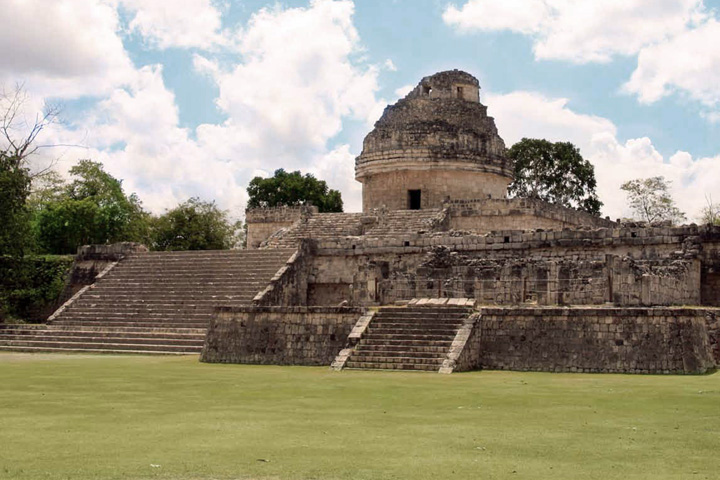
\includegraphics[width=\marginparwidth]{figures/caracol.jpg}
 % \label{fig:caracol}
%\end{marginfigure}









%agregar a forma final\cleardoublepage
%\ctparttext{You can put some informational part preamble text here.}
\part{Ecuación de Schrödinger Dependiente del Tiempo}\label{pt:TDSE}

%************************************************
\chapter{Marco histórico}\label{ch:MarcoHistorico1}
% ************************************************

\section{Primeros telescopios y observatorios}

\section{Resultados importantes}
% importancia de los detectores
%************************************************
\chapter{Representación de Variable Discreta}\label{ch:DVR}
% ************************************************
Existen diferentes métodos numéricos para resolver la ecuación de Schrödinger Dependiente del Tiempo (\autoref{eq:TDSE ket}). En esta capítulo se desarrollará un método particular conocido como el método de \textbf{Representación de Variable Discreta}, \acs{DVR} por sus siglas en inglés.
\\\\
Formalmente, el espacio de Hilbert de las funciones de onda es infinito, sin embargo, para resolver y tratar problemas de numéricamente, es necesario hacer un truncamiento de la dimensión del espacio a un número finito $N$. Este espacio reducido de Hilbert, puede verse como un espacio generado por un operador de proyección, además, el espacio reducido de Hilbert tiene el mismo formalismo de la mecánica cuántica, pues, si se recuerda que la dimensión del espacio de Hilbert está dado por las distintas alternativas que puede tomar el sistema cuántico en cuestión, este espacio de dimensión $N$, puede ser un espacio completo para otro problema en mecánica cuántica.

\section{Proyección Espectral}
Una función de onda y sus operadores se pueden representar mediante una una base de funciones ortogonales, a esta base se le conoce como \textbf{base espectral}:
$$\{\phi_i(x)\}_{i=1}^{N}$$
que, por ser funciones ortogonales cumplen que:
$$\bra{\phi_i(x)}\ket{\phi_j(x)} = \delta_{ij}$$
Como se mencionó anteriormente, la dimensión del espacio de Hilbert se debe reducir a un número finito $N$, esta reducción de dimensión se puede expresar mediante un \textbf{operador de proyección}:

\begin{equation}
  \label{eq:operadorproyeccion}
  P_N = \sum_{n=1}^N\ket{\phi_n}\bra{\phi_n}
\end{equation}

Mediante el operador $P_N$ se puede mapear la dinámica del espacio de Hilbert al espacio reducido de Hilbert, en particular, es de interés para resolver la \autoref{eq:TDSE ket} conocer cómo se representa el operador Hamiltoniano:
\begin{equation}
  \label{eq:Hamiltoniano}
  H = \frac{\hat{p}^2}{2m}+V(\hat{x})
\end{equation}

Utilizando la base espectral, el Hamiltoniano en el espacio reducido de Hilbert se puede representar como:

\begin{equation}
  \label{eq:Hamiltonianored}
  H_N = P_NHP_N
\end{equation}

Definiendo $Q_N = 1-P_N$, la Ecuación de Schrödinger Dependiente del Tiempo se puede escribir en términos de $P_N$ y $Q_N$ como un conjunto de dos ecuaciones diferenciales acopladas:

\begin{equation}
  \label{eq:acopladas1}
  i\hbar\frac{\partial \psi_N}{\partial t} = P_NHP_N\psi_N + P_NHQ_N\psi_{\perp}
\end{equation}
\begin{equation}
  \label{eq:acopladas2}
  i\hbar\frac{\partial \psi_{\perp}}{\partial t} = Q_NHP_N\psi_N + Q_NHQ_N\psi_{\perp}
\end{equation}


en donde: $\psi_N = P_N\psi$ y $\psi_{\perp}=Q_N\psi$.
\\

Para este trabajo se usará la aproximación de Galerkin \cite{Gottlieb}, en donde se desprecia la contribución de $\psi_{\perp}$, de esta forma, la Ecuación de Schrödinger Dependiente del Tiempo a resolver es:
\begin{tcolorbox}[colback=CTtitle!5!white,colframe=CTtitle!85!white]%,title=\centering{Ecuación de Schrödinger Dependiente del Tiempo para un estado}]
\begin{equation}
\label{eq:TDSEN}
i\hbar \frac{\partial \psi_N}{\partial t} = P_NHP_N\psi_N
\end{equation}
\end{tcolorbox}

\subsection{Representación de la Función de Onda}

Una función de onda $\psi(x)$ se puede escribir como una suma infinita en términos de funciones ortonormales $\phi_i$:
\begin{equation}
  \label{eq:wavefuninf}
  \psi(x) = \sum_{n=1}^{\infty}a_n\phi_n(x)
\end{equation}
con:
\[ \int \phi_m^*(x)\phi_n(x)dx = \delta_{mn} \]
\[ a_n = \int \phi_n^*(x)\psi(x)dx\]
para $m,n=1,2,3,\dots, \infty$.
\\
\\
Utilizando la definición del operador de proyección de la \autoref{eq:operadorproyeccion}, se puede probar que:
\begin{equation}
  \label{eq:wavepacketinit}
  \psi_N(x) = P_N\psi(x)=\sum_{n=1}^{N}a_n\phi_n(x)
\end{equation}

\subsection{Colocación del Operador de Proyección}
Dado un conjunto de puntos en el espacio de posiciones: $\{x_i\}$ con $i=1,2,3,\dots N$, la siguiente relación:
\begin{equation}
  \label{eq:wavefunexp}
  \psi_N(x_i) = P_N\psi(x_i)=\sum_{n=1}^{N}b_n\phi_n(x_i) = \psi(x_i)
\end{equation}

está asociada a la \textbf{colocación}\footnote{Los \textbf{métodos de colocación} son soluciones numéricas de un conjunto de ecuaciones, cuya solución resulta ser exacta en un conjunto discreto de puntos llamados puntos de colocación.\cite{Tannor:2006}} del operador de proyección, y los puntos $\{x_i\}$ son llamados \textbf{puntos de colocación}. Los coeficientes $b_n$ están determinados por la condición de que: $\psi_N(x)=\psi(x)$ en el conjunto de puntos de colocación.


\section{Base Pseudo-espectral}
Una \textbf{base pseudo-espectral}: $\{\theta_j\}_{j=1}^N$ se define como la base de las funciones localizadas espacialmente. La base de funciones ortogonales $\{\phi_n\}_{n=1}^N$, la colocación en la \autoref{eq:wavefunexp}, los puntos de colocación $\{x_i\}_{i=1}^N$, y los factores de peso definidos como $\Delta_j$ con $j=1,\dots,N$, determinan completamente la forma de la base pseudo-espectral:

\begin{equation}
  \label{eq:basepseudo}
  \theta_j(x) \equiv \sum_{n=1}^N\phi_n(x)\Phi_n^*(x_j)
\end{equation}
donde:
$$\Phi_n(x_j)\equiv \sqrt{\Delta_j}\phi_n(x_j)$$
$$\theta_j(x_i) = \Delta_j^{-1/2}\delta_{ij}$$


En conjunto, las $N$ funciones de la base pseudo-espectral generan el mismo espacio de Hilbert reducido que las $N$ funciones ortogonales de la base espectral, y ambas bases están relacionadas mediante una transformación unitaria: $\Phi_n^*$. Como consecuencia, se tiene que el operador de proyección es idéntico en ambas bases, es decir:
\begin{equation}
  \label{eq:proyecbases}
  P_N = \sum_{n=1}^N\ket{\phi_n}\bra{\phi_n}=\sum_{j=1}^N\ket{\theta_j}\bra{\theta_j}
\end{equation}

Se puede probar \cite{Tannor:2006}, que tanto la base espectral, como la base pseudo-espectral tienen propiedades de completes y ortogonalidad completamente análogas. Esto es de particular importancia, pues, dado que ambas bases generan el mismo espacio reducido de Hilbert, los operadores se pueden escribir tanto en términos de una base, como en la otra, y, si es necesario hacer cálculos con estos operadores (como sumarlos), se puede utilizar la transformación unitaria para escribirlos en términos de la misma base.


\section{Algoritmo DVR aplicado a un proceso físico-químico}\label{sec:DVRapp}

En esta sección se aplicarán los conceptos revisados a lo largo del capítulo para resolver un problema físico-químico que involucra potenciales dependientes del tiempo utilizando el método \acs{DVR}.\\
La implementación numérica se realizó en Python 3.9.7 y se encuentra disponible en el repositorio: \href{https://github.com/Jessi-MM/PropagatorLearning/blob/main/src/ANN_as_Propagators_DidacticNotebook.ipynb}{\faGithub Transferencia de Protones}

\subsection{Sistema de Transferencia de Protones}\label{sec:ProtonTransfer}

Los sistemas de \textbf{transferencia de protones} ocurren en un complejo de enlaces de hidrógeno: $A-H\dotsb A'$. El modelo simplificado se muestra en la siguiente figura:

\begin{figure}[ht]
  \centering
\includegraphics[width=0.6\textwidth]{/home/jessica/Tesis/img/DrawModel.png}
\caption{Descripción del modelo de transferencia de protones $H^+$.}
\label{fig:drawmodel}
\end{figure}

En donde la coordenada $Q$ hace referencia a la separación entre los átomos $A$ y $A'$, mientras que la coordenada $r$ es la distancia del protón al centro de los enlaces. \cite{DynamicalTheoryPTS}. \\
En las descripciones teóricas de la transferencia de protones, a menudo el hidrógeno es representado moviéndose a través de un pozo de doble potencial unidimensional. \cite{Enzymes}
\\

A continuación se presenta un modelo particular de potencial para el sistema de transferencia de protones, en donde la descripción está dada por la coordenada del protón $r \in [-1.5 \,\,\mathring{A}, 1.5 \,\,\mathring{A}]$. A cada tiempo $t$ el valor del potencial $V(r,t)$ está dado por el eigenvalor más bajo de la siguiente matriz:

\begin{equation}
  \label{eq:matrixPot}
  \begin{pmatrix}
    U_1(r,R(t)) &   V \\
    V           & U_2(r,R(t))+X(t)
  \end{pmatrix}
\end{equation}

En donde $U_1(r,R(t))$ y  $U_1(r,R(t))$ son potenciales de oscilador armónico, y $V$ es una constante.

\begin{equation}
  \label{eq:U1}
  U_1(r,R(t))=\frac{1}{2}m\omega_1^2\left( r + \frac{R(t)}{2} \right)
\end{equation}

\begin{equation}
  \label{eq:U2}
  U_2(r,R(t))=\frac{1}{2}m\omega_2^2\left( r - \frac{R(t)}{2} \right)
\end{equation}

En las ecuaciones de potenciales de oscilador armónico, $m$ se refiere a la masa del protón, $\omega$ es la frecuencia del pozo de protones. Los términos $U_1(r,R(t))$ y  $U_1(r,R(t))$ están desplazados mediante un término de energía dependiente del tiempo: $X(t)$, y un termino de distancia dependiente del tiempo: $R(t)$. La dinámica de $X(t)$ corresponde a las fluctuaciones del entorno, mientras que $R(t)$ representa las vibraciones de los sitios donantes y aceptores de protones. \cite{Main:2021}

\begin{equation}
  \label{eq:X(t)}
  X(t)=\lambda \cos(\omega_xt+\theta_x)+X_{eq}
\end{equation}

\begin{equation}
  \label{eq:R(t)}
  R(t)=(R_0-R_{eq})\cos(\omega_Rt + \theta_R) + R_{eq}
\end{equation}

\begin{figure}[ht]
  \centering
  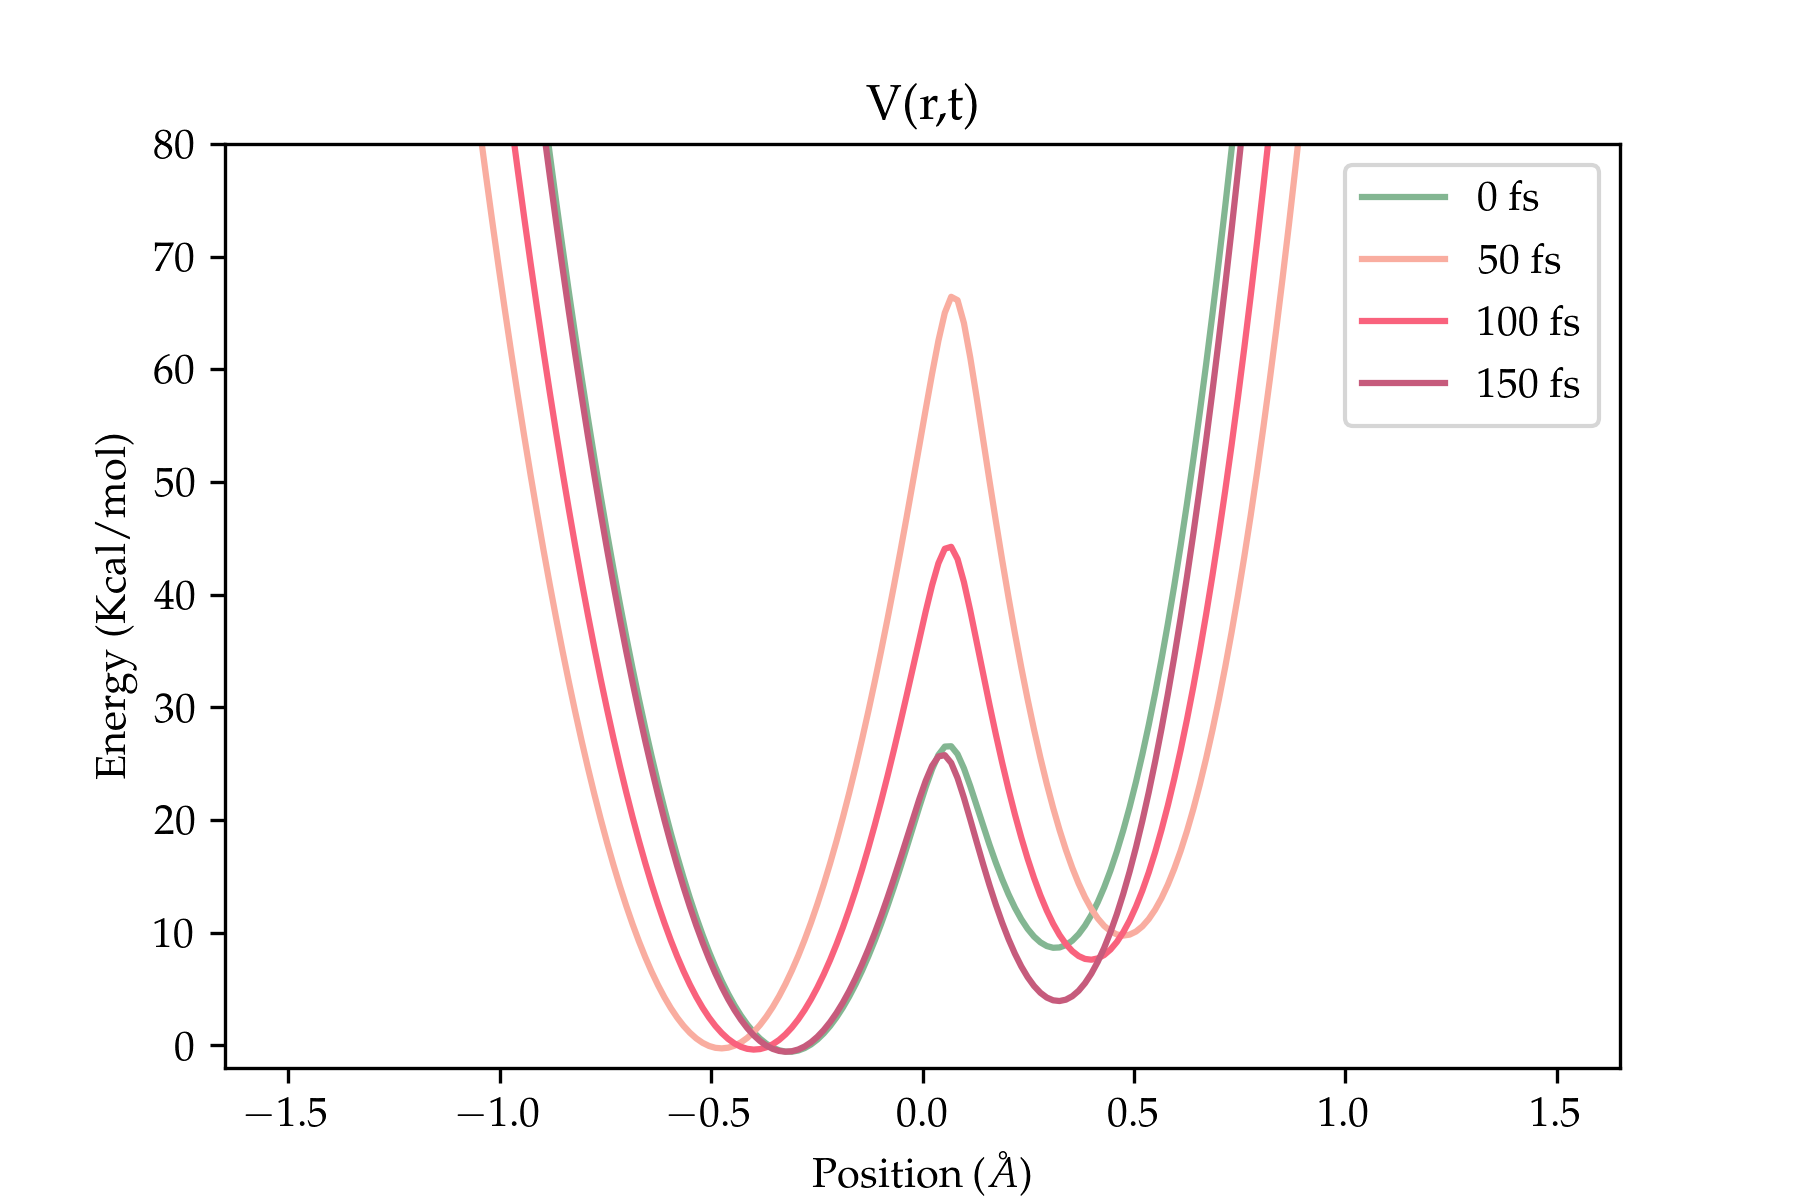
\includegraphics[width=1\textwidth]{/home/jessica/Tesis/img/tesis/ExamplesPotential1.png}
  \caption{Potencial $V(r,t)$ a diferentes tiempos.}
  \label{fig:drawPot}
\end{figure}

La \autoref{fig:drawPot} muestra un ejemplo de potencial $V(r,t)$ generado con la implementación de las ecuaciones anteriores. Los parámetros de potencial utilizados se muestran en la \autoref{tab:ValuesPlot1}

\subsection{Elección de una base Ortonormal y Grid}

Para proceder con la solución a la \acs{TDSE} \autoref{eq:TDSE ket}, elegimos una base de funciones ortogonales: \cite{Colbert1992}

\begin{equation}
  \label{eq:eigenfunc}
  \phi_n(r)=\sqrt{\frac{2}{b-a}}\sin\left( \frac{n\pi(r-a)}{b-a}\right) \,\,\,\,\, n=1,..,N
\end{equation}

y un grid en el espacio de posiciones:
\begin{equation}
  \label{eq:grid}
  r_i = a + \frac{(b-a)i}{N-1} \,\,\,\,\, i=0,..,N-1
\end{equation}

donde: $a=-1.5\AA$, $b=1.5\AA$ y $N=200$ para la implementación numérica, es decir, que el espacio reducido de Hilbert del sistema tiene una dimensión de $N=200$. La \autoref{fig:Phi_n} muestra las primeras cinco funciones ortogonales de la base en el grid del espacio de posiciones. Las funciones $\phi_n$ están construidas para que se cumpla: $\phi_n(r=r_0=a)=\phi_n(r=r_{N-1}=b)=0$.

\begin{figure}[ht]
  \centering
  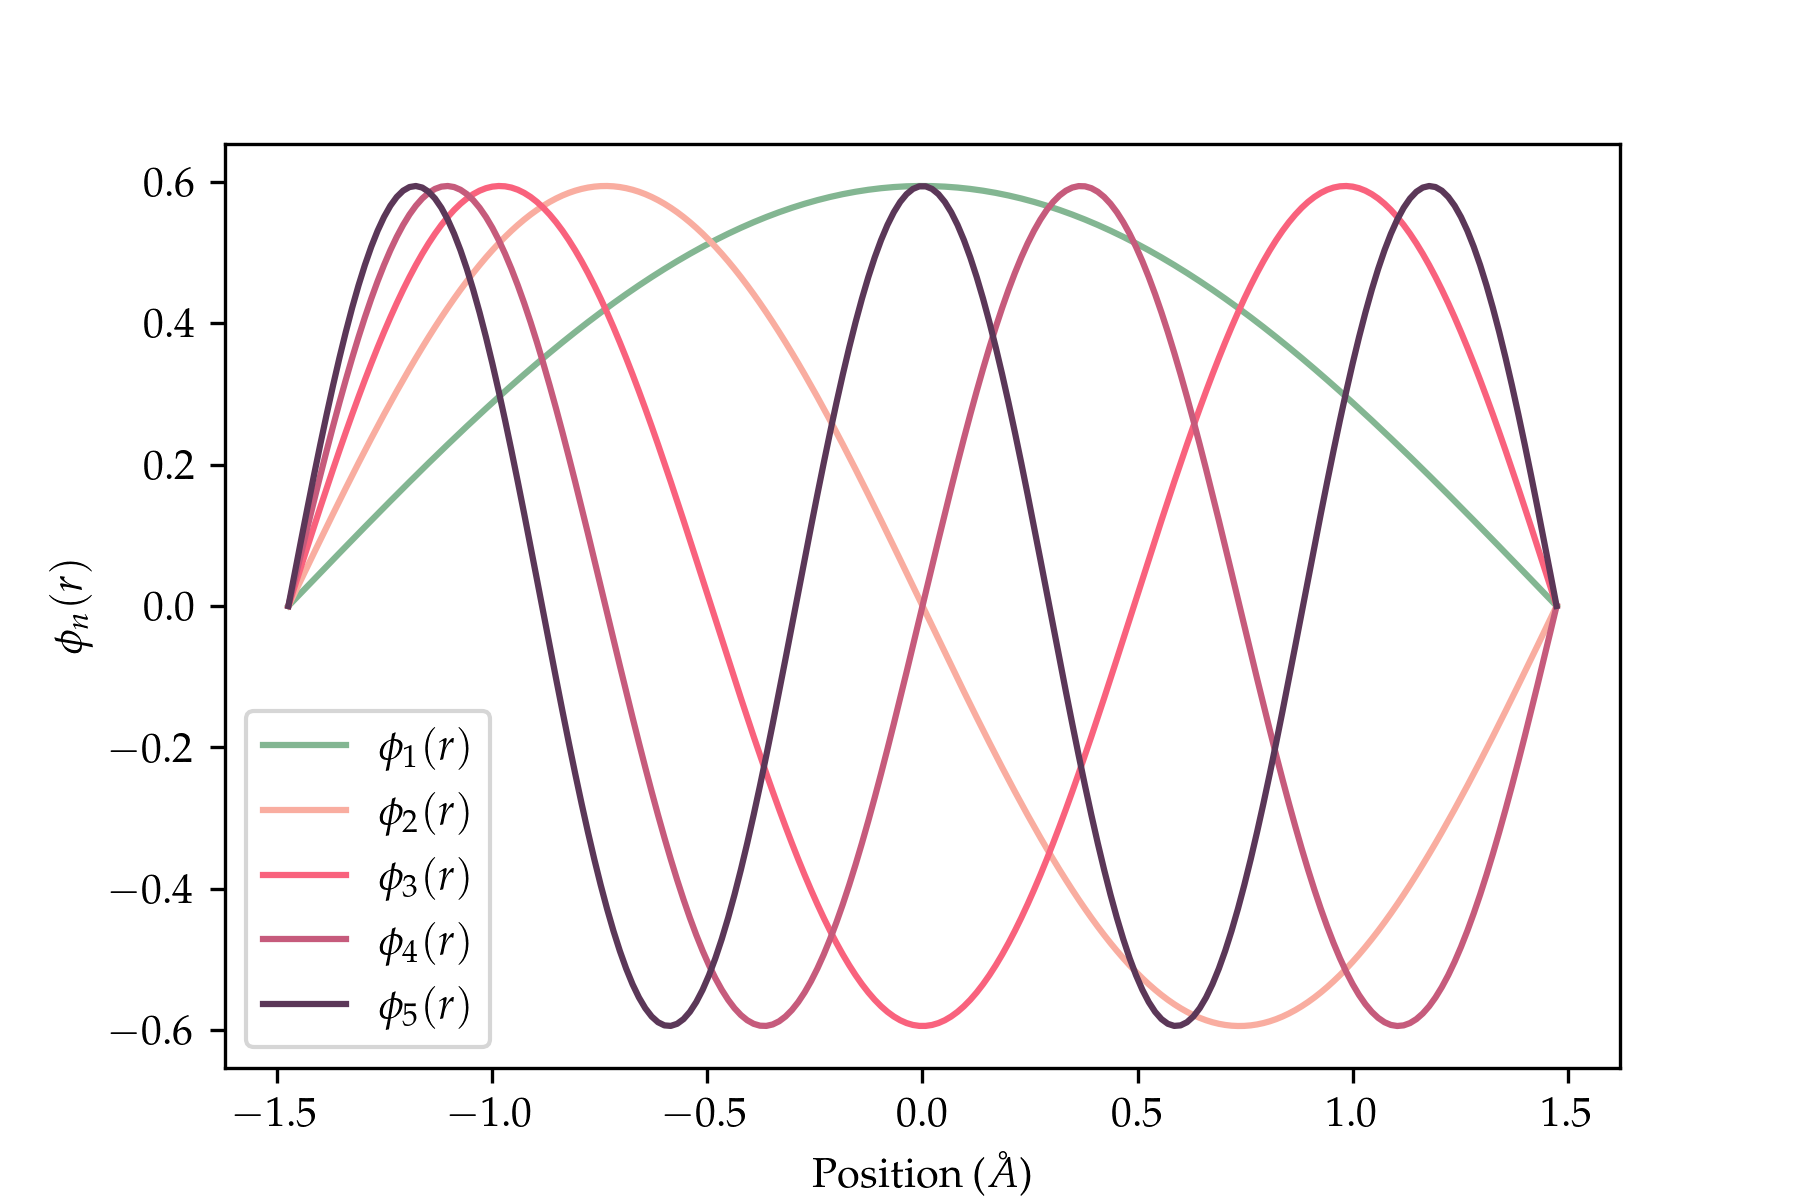
\includegraphics[width=1\textwidth]{/home/jessica/Tesis/img/tesis/Phi_n1.png}
  \caption{Funciones ortogonales $\phi_n(r)$ en el grid $\{r_i\}_{i=0}^{N-1}$ para $n=1,..5$.}
  \label{fig:Phi_n}
\end{figure}

\subsubsection{Representación de la matriz del Hamiltoniano en la Base Espectral}

Los elementos de matriz de la Energía Cinética en la base pseudo-espectral están dados por:
\begin{equation}
  \label{eq:T}
T^{\theta}_{ij}= \bra{\theta_i}T\ket{\theta_j}=\sum_{n=1}^N\bra{\theta_i}\ket{\phi_n}\bra{\phi_n}T\ket{\theta_j}
\end{equation}
realizando la aproximación:
$$\bra{\theta_j}T\ket{\phi_n} \approx \bra{r_j}T\ket{\phi_n}$$
y considerando que el operador $T$ en el espacio de posiciones $r$ está dado por:
\begin{equation}
  \label{eq:Toperator}
  T = -\frac{\hbar^2}{2m}\frac{d^2}{dr^2}
\end{equation}


se puede obtener que: \cite{Tannor:2006}\cite{Colbert1992}
\begin{equation}
  \label{eq:T_DVR}
  T^{\theta}_{ij}\approx -\frac{\hbar^2}{2m}\Delta r\sum_{n=1}^{N}\phi_n(r_i)\frac{\partial^2\phi_n}{\partial r^2}\biggr\rvert_{r_j}
\end{equation}

donde: $\Delta r = (b-a)/N-1$. Obteniendo la segunda derivada de la \autoref{eq:eigenfunc}, y sustituyendo en la \autoref{eq:T_DVR} se tiene:

\begin{equation}
  \label{eq:T_N}
  T^{\theta}_{ij}=\frac{\hbar^2}{2m}\left(\frac{\pi}{b-a} \right)^2\frac{2}{N-1}\sum_{n=1}^Nn^2\sin\left(\frac{n\pi i}{N-1} \right)\sin\left(\frac{n\pi j}{N-1} \right)
\end{equation}

que son los elementos de matriz de la Energía Cinética en la base pseudo-espectral, $T^{\theta}\in \mathcal{M}_{200\times200}(\mathbb{R})$.
\\
\\
La representación de la matriz de Energía Potencial en la base pseudo-espectral es más simple que la de la Energía Cinética, pues 
las funciones $\{\theta_i\}$ son localizadas en el espacio de posiciones $r$ y cumplen la condición de ortogonalidad: $\bra{\theta_i}\ket{\theta_j}= \delta_{ij}$, así:

\begin{equation}
  \label{eq:V_DVR}
  V^{\theta}_{ij}= \bra{\theta_i}V(\hat{r})\ket{\theta_j}=V(r_i)\delta_{ij}
\end{equation}

$V^{\theta}\in \mathcal{M}_{200\times200}(\mathbb{R})$ es una matriz diagonal.
\\
Dado un tiempo $t$, los elementos de la diagonal $V^{\theta}_{ii}$ están dados por $V(r_i,t)$ (\autoref{eq:matrixPot}), con $i=0,..,31$.
\\
A partir de la \autoref{eq:T_N} y \autoref{eq:V_DVR}, se construye la matriz del Hamiltoniano en la base pseudo-espectral al tiempo $t$:
\begin{equation}
  \label{eq:H_DVR}
  H(t)^{\theta} = V(t)^{\theta}+T^{\theta}
\end{equation}
en donde el Hamiltoniano tiene dependencia temporal debido a que el Potencial del sistema es dependiente del tiempo.

\subsection{Propagación de un Paquete de Onda}

Sea un paquete de onda al tiempo $t=0$ (\autoref{fig:psi_0}): 
\begin{equation}
  \label{eq:psi_0}
\psi(r,0)=\sum_{i=1}^{k=5}C_i \cdot \phi_{i}(r)
\end{equation}
con $C_i$ números complejos aleatorios de una distribución uniforme, y elegidos de tal forma que: $\bra{\psi(r,0)}\ket{\psi(r,0)}=1$
\begin{figure}[!htbp]
  \centering
  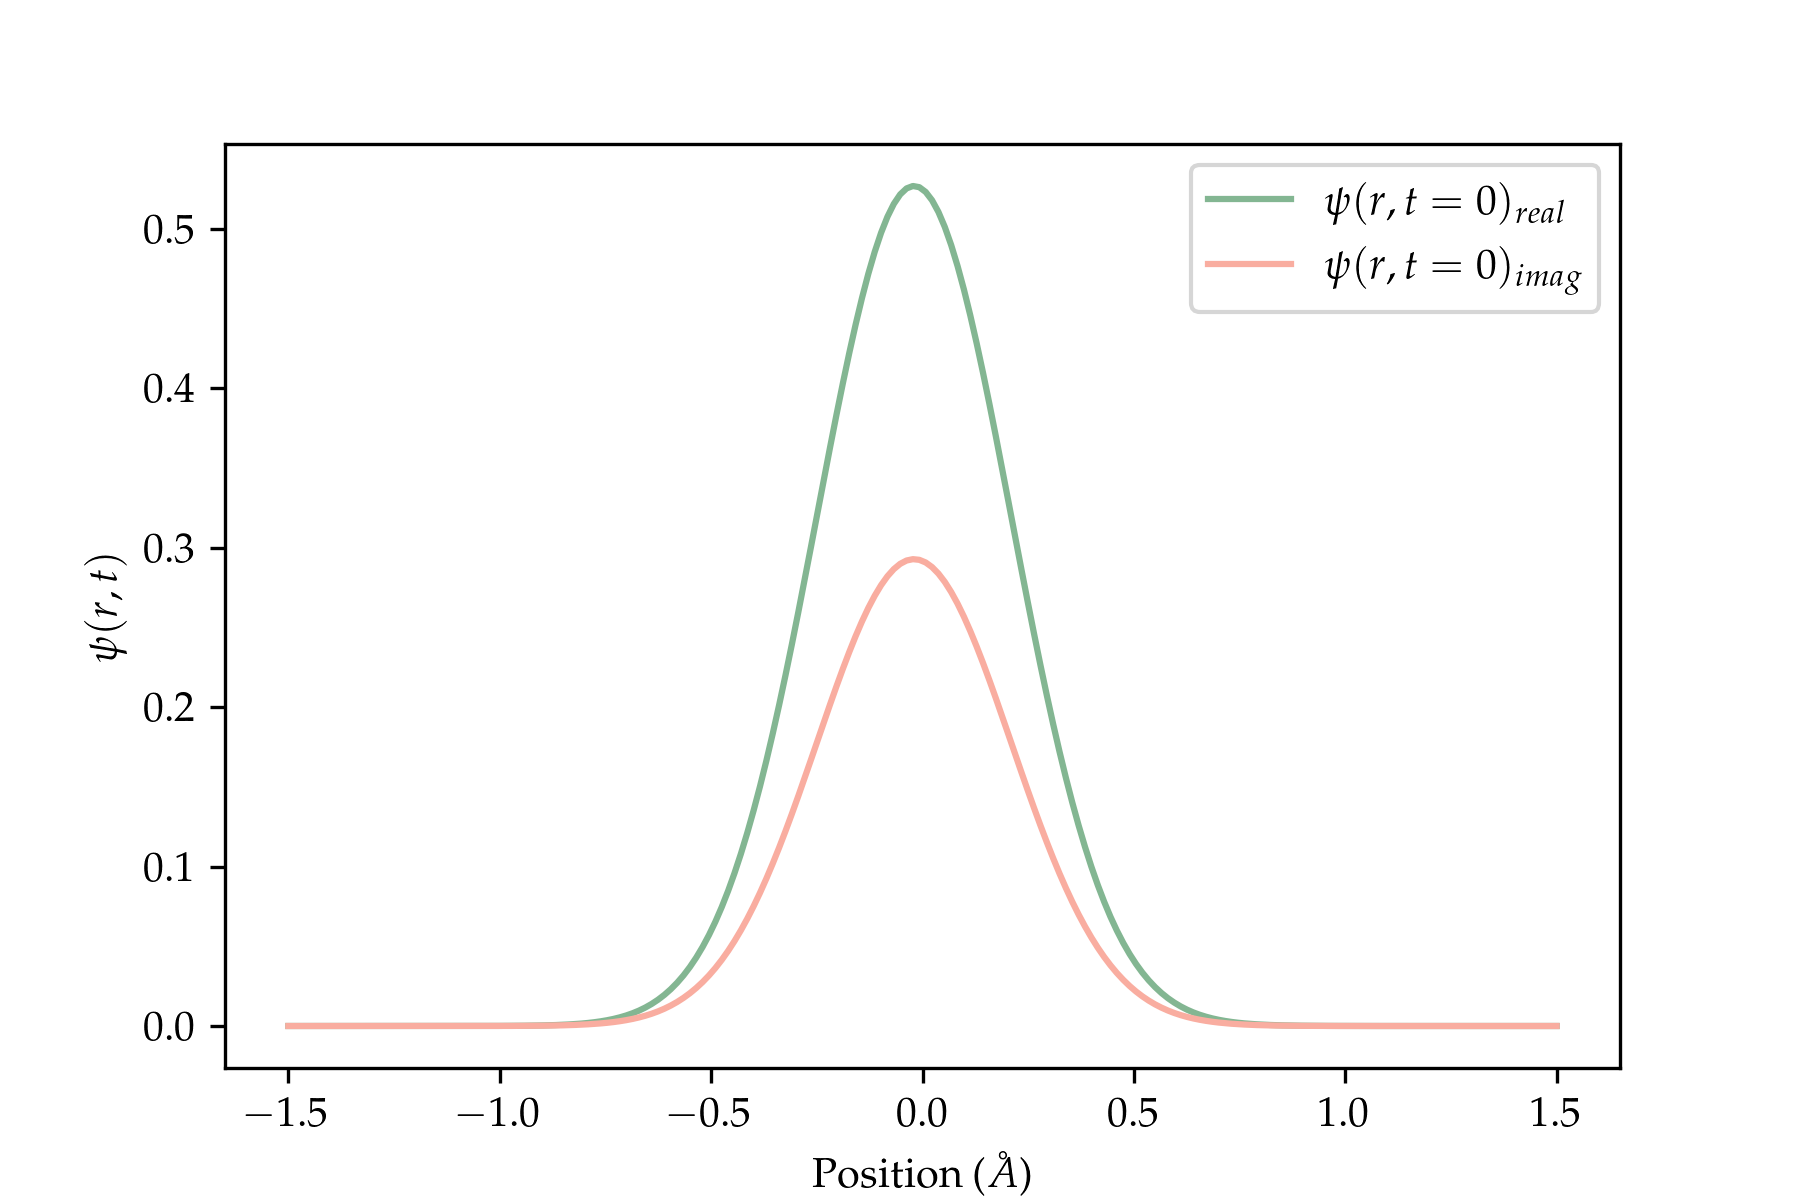
\includegraphics[width=0.9\textwidth]{/home/jessica/Tesis/img/tesis/psi_01}
  \caption{Paquete inicial de onda al tiempo $t=0$. Parte real y compleja.}
  \label{fig:psi_0}
\end{figure}

Si se toma un intervalo de tiempo $\Delta t$ lo suficientemente pequeño como para que el potencial se pueda considerar constante en ese intervalo de tiempo ($\approx 1\,\,fs$ para el sistema en cuestión), la evolución temporal del paquete de onda está dado por (\autoref{eq:U IT}):
\begin{equation}
  \label{eq:wp_ev}
  \psi(r,t)=\exp{-iH^{\theta}t/\hbar}\psi(r,0)
\end{equation}

Si $H^{\theta} = UDU^{-1}$, con $D$ una matriz diagonal:
$$ \psi(r,t) = \exp{-iUDU^{-1}t/\hbar}\psi(r,0)$$  
así,
\begin{equation}
  \label{eq:psi_t}
\psi(r,t) = U\exp{\frac{-it}{\hbar}D}U^{-1}\psi(r,0)
\end{equation}

En donde la matriz $U$ está formada por los $N$ eigenvectores de $H^{\theta}$ como vectores columna, y:
$$D=U^{-1}H^{\theta}U$$.
\\

La \autoref{fig:psi_ev} muestra la evolución de la parte real del paquete de onda en intervalos de $1\,fs$ a lo largo de $5\,fs$, obtenida con la \autoref{eq:psi_t}. En la \autoref{fig:dens_ev} se muestra la evolución temporal de la densidad del protón.\\
\href{https://github.com/Jessi-MM/PropagatorLearning/blob/main/src/Animacion/gifs/animation-dens\%26pot.gif}{\faPlayCircle[regular] Evolución Temporal: Potencial y Densidad}

\begin{figure}[!htbp]
  \centering
  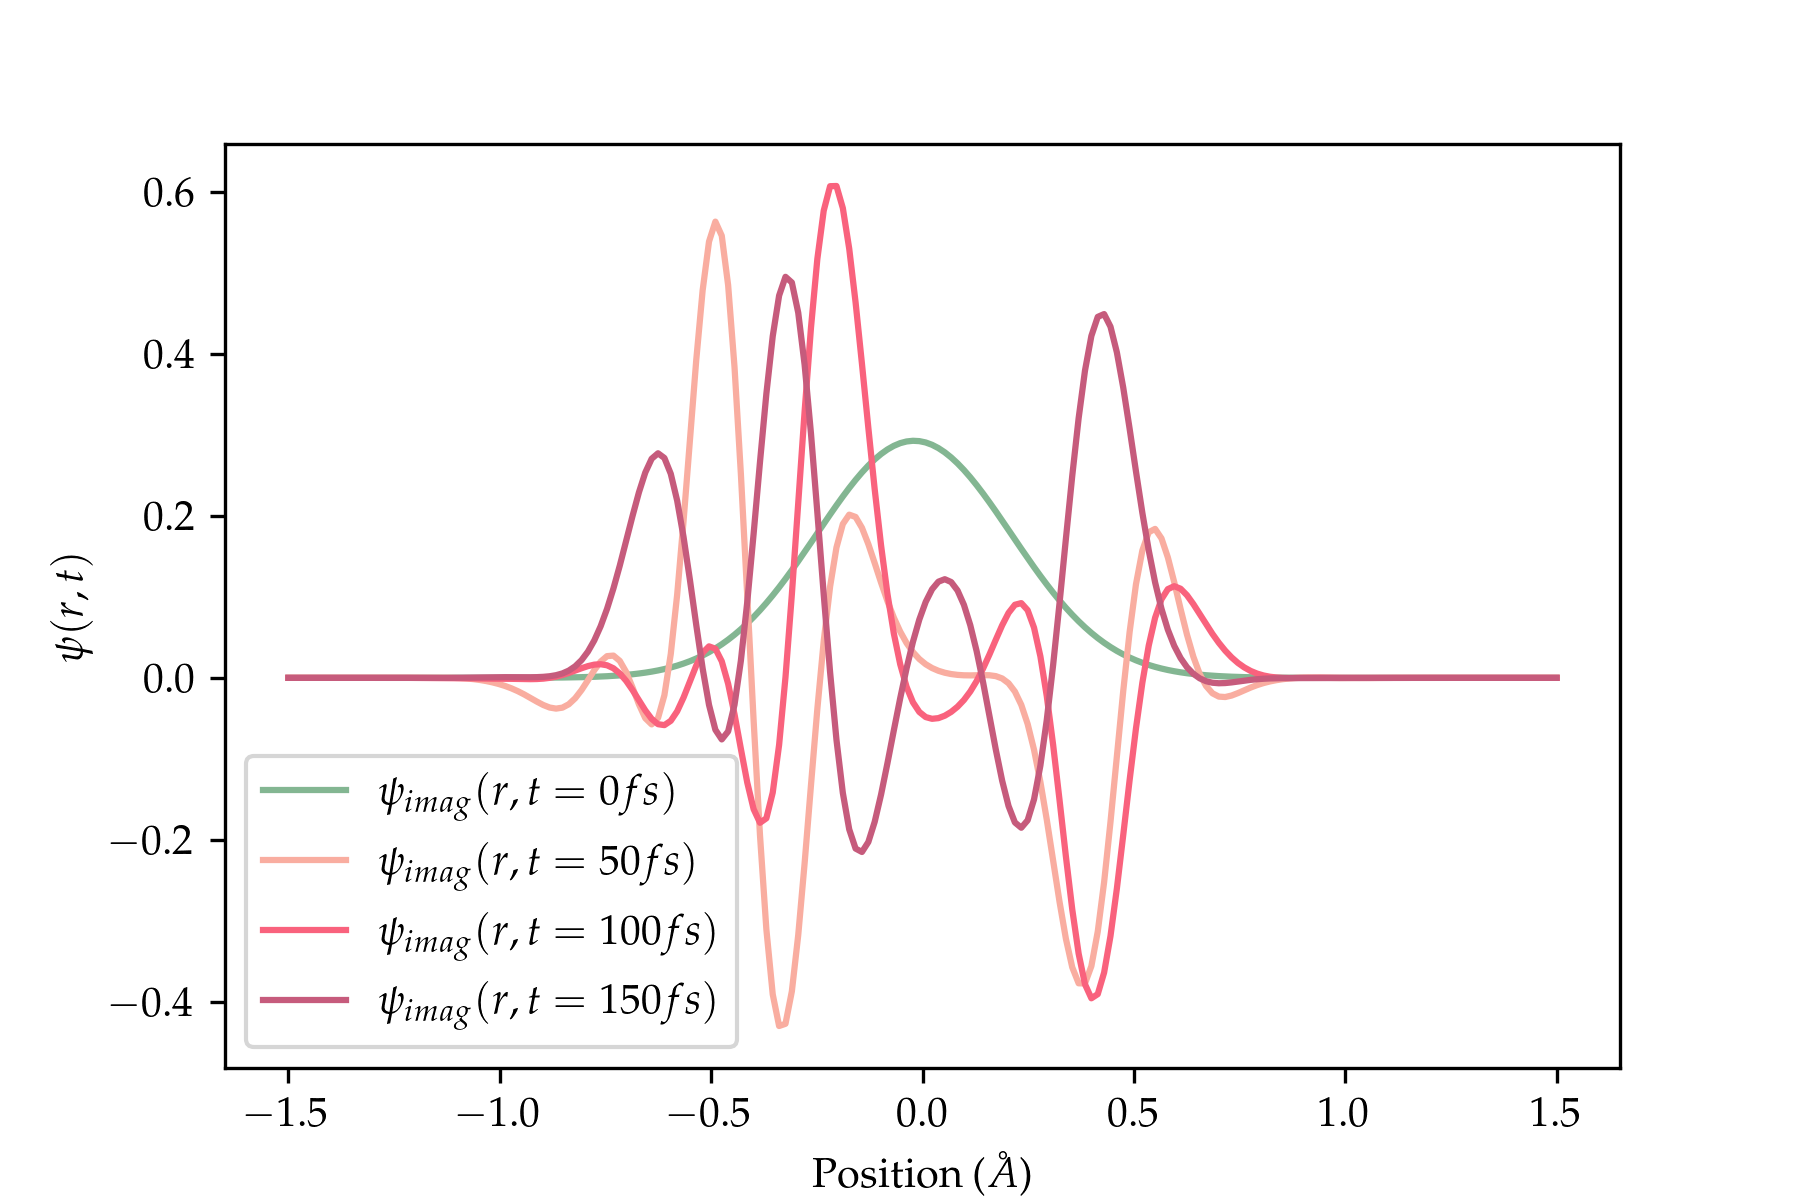
\includegraphics[width=1\textwidth]{/home/jessica/Tesis/img/tesis/psi_ev1real}
  \caption{Propagación del paquete de onda $\psi(r,t)$ parte real.}
  \label{fig:psi_evre}
\end{figure}

\begin{figure}[!htbp]
  \centering
  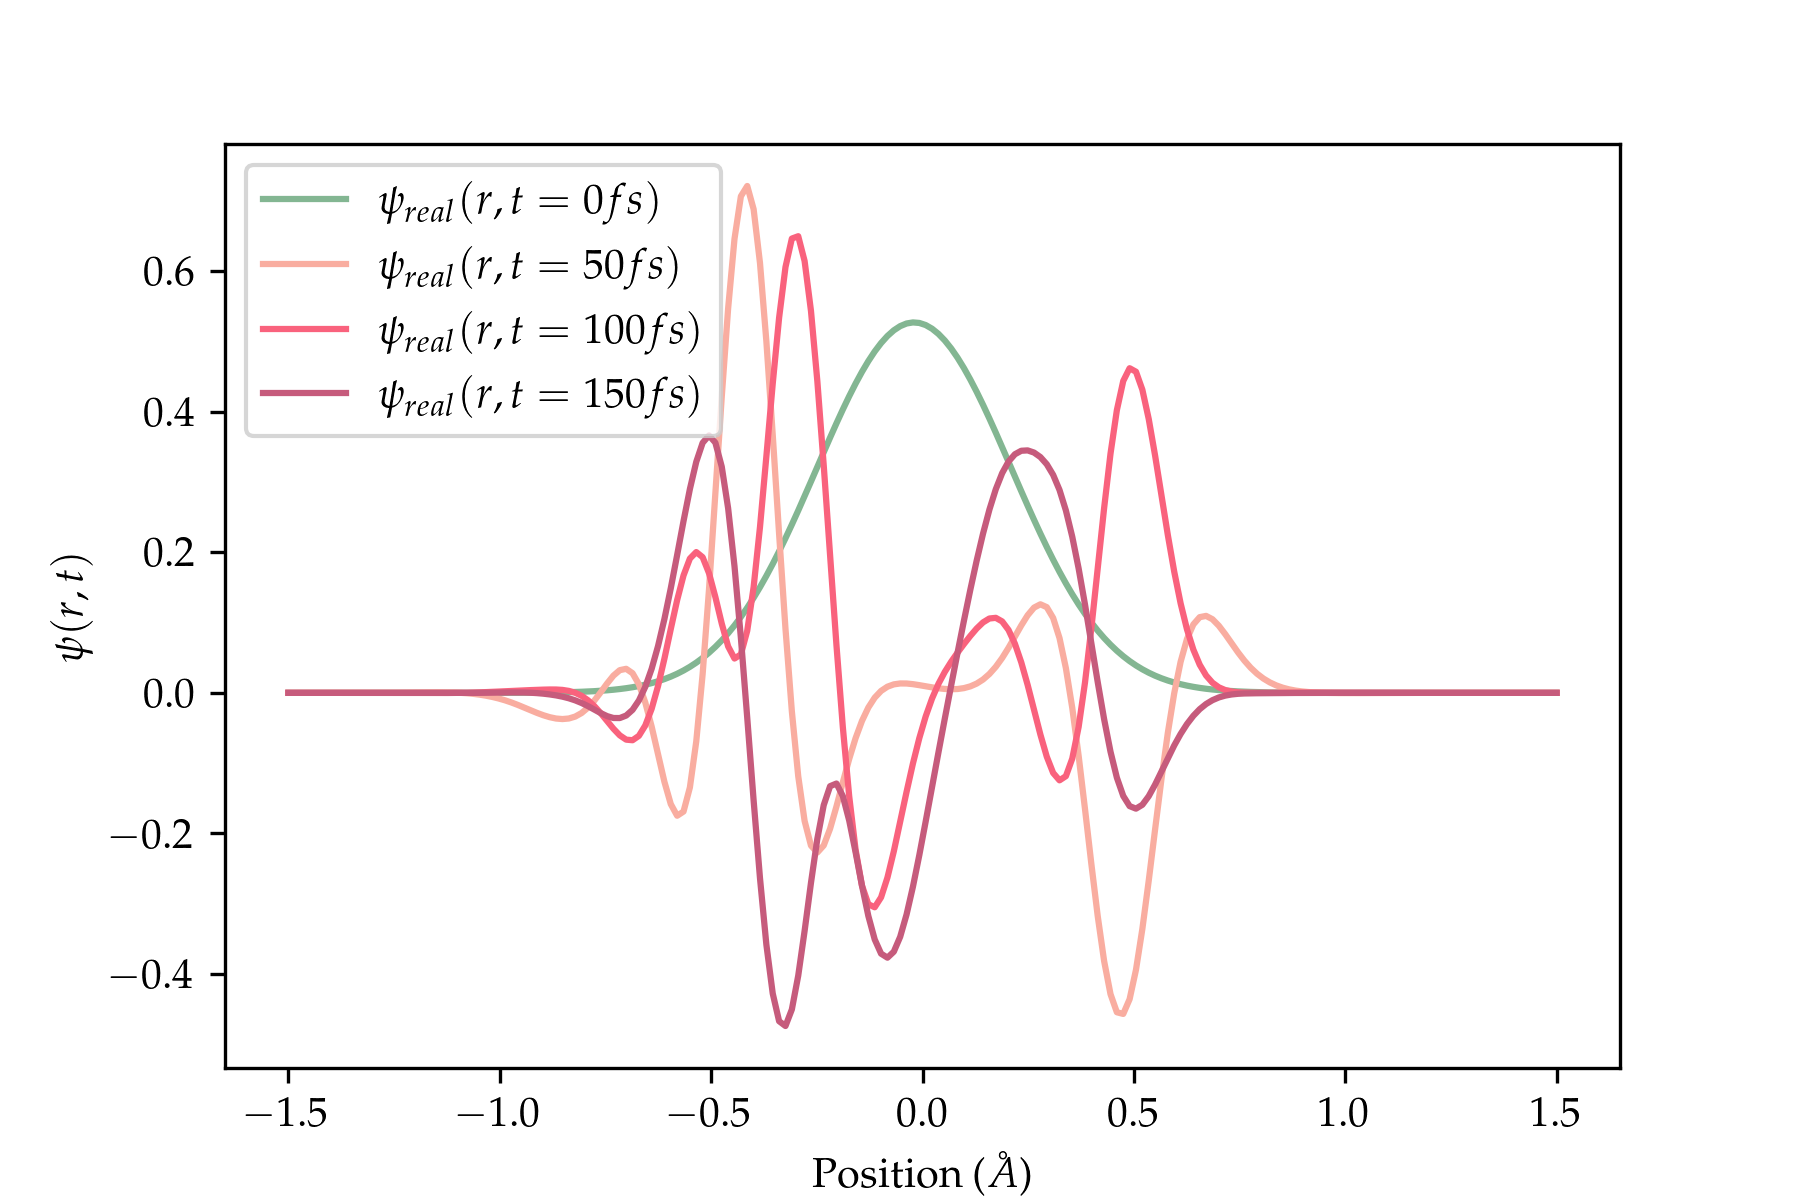
\includegraphics[width=1\textwidth]{/home/jessica/Tesis/img/tesis/psi_ev1imag}
  \caption{Propagación del paquete de onda $\psi(r,t)$ parte imaginaria.}
  \label{fig:psi_evim}
\end{figure}

\begin{figure}[!htbp]
  \centering
  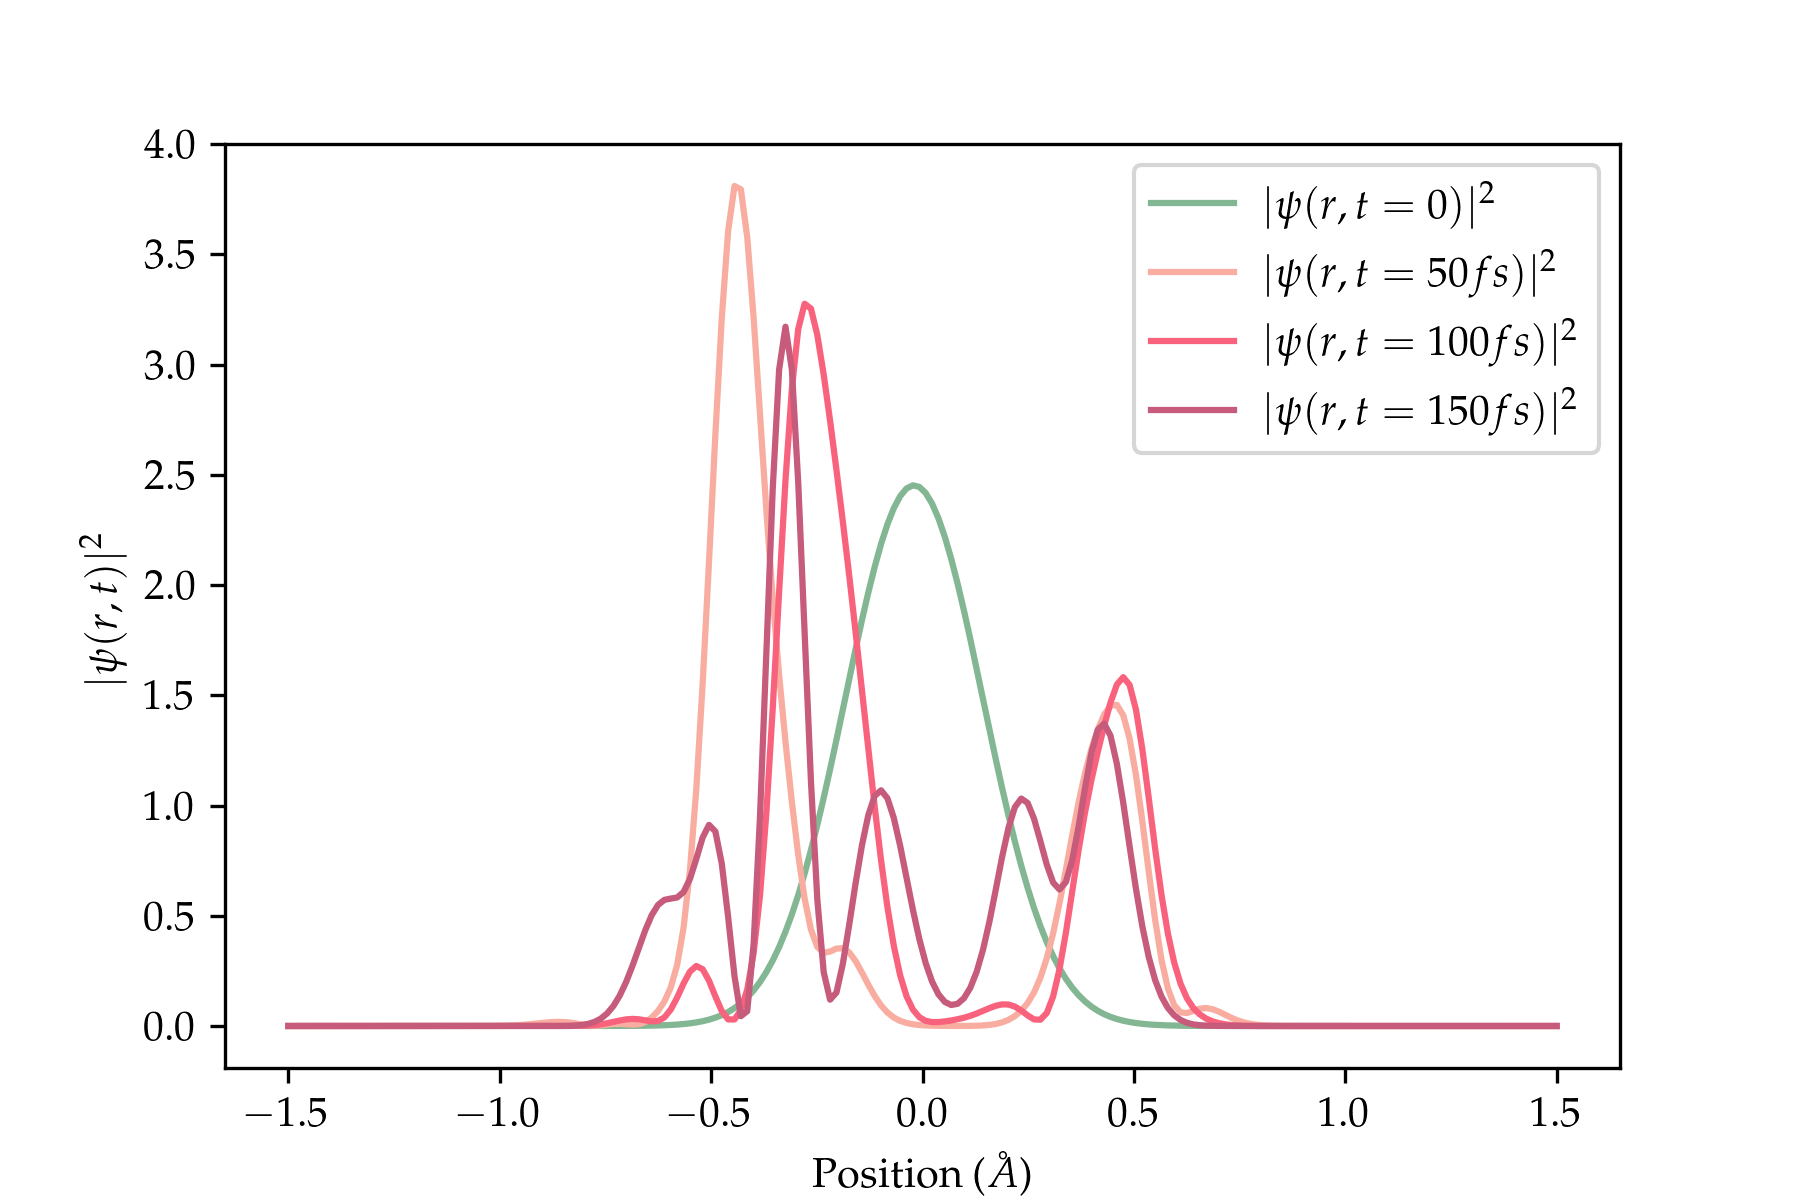
\includegraphics[width=1\textwidth]{/home/jessica/Tesis/img/tesis/dens_ev1}
  \caption{Evolución temporal de la densidad $|\psi(r,t)|^2$.}
  \label{fig:dens_ev}
\end{figure}



%agregar a forma final \cleardoublepage
%\ctparttext{You can put some informational part preamble text here.}
\part{Redes Neuronales Artificiales (ANN's)}\label{pt:ANNS}

%************************************************
\chapter{Aprendizaje automático}\label{ch:ML}
% ************************************************
%--- Deep Learning Ian G book
% Historical dev
% big data &  improve of memorie in computer
% poner el puto diagramita q siempre sale

%\begin{flushright}{\slshape
 %   El aprendizaje automático es como una caja de bombones: nunca sabes lo que vas a obtener... a menos que tengas buenos datos y una sólida comprensión de tus algoritmos.} \\ \medskip
  %  --- ChatGPT AI language model
%\end{flushright}



La \textbf{inteligencia artificial}, o AI por sus siglas en inglés, se puede definir como un sistema capaz de interactuar con su entorno. Algunos ejemplos de inteligencias artificiales son: \emph{Siri} de Apple y \emph{Alexa} de Amazon. Para poder generar una respuesta al entorno, estos sistemas contienen sensores que permiten la entrada de información, en estos ejemplos la información es obtenida mediante la voz o las palabras escritas de los usuarios, esta información es procesada a través de métodos de aprendizaje automático o ML por sus siglas en inglés.

\begin{figure}[!htbp]
  \centering
  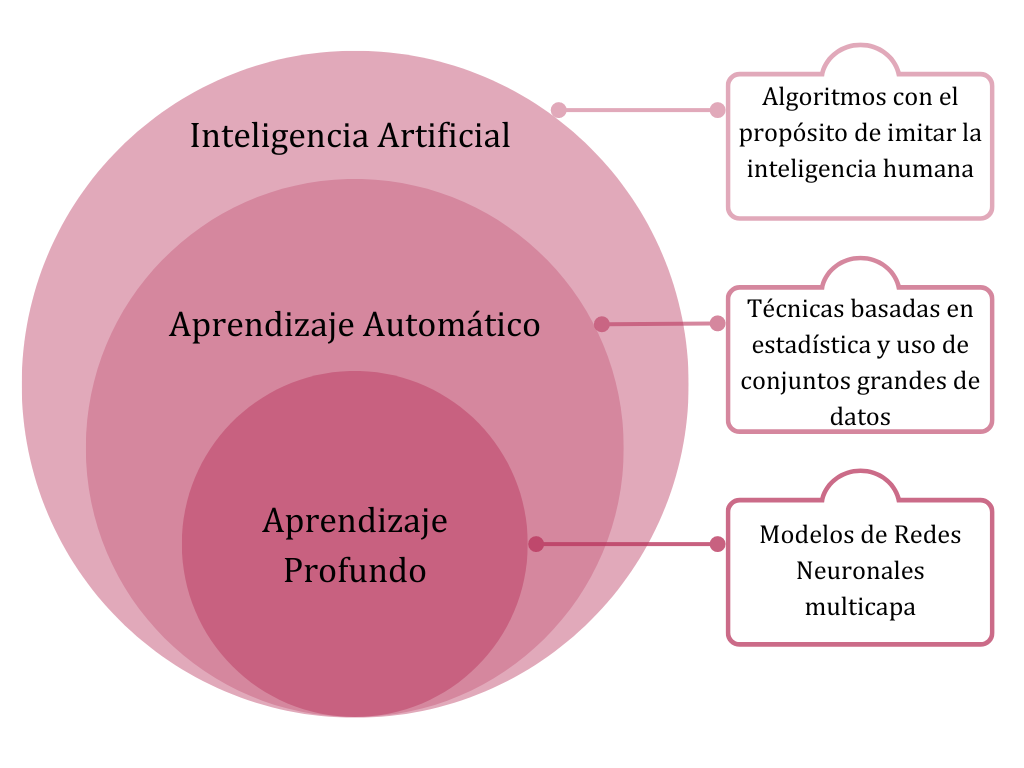
\includegraphics[width=0.7\textwidth]{./img/IA_ML_DL.png}
  \caption{Diagrama de Venn que muestra los conceptos de inteligencia artificial, aprendizaje automático y aprendizaje profundo.}
  \label{fig:IA-ML-DL}
\end{figure}

Los métodos de \textbf{aprendizaje automático} se pueden definir como un conjunto de métodos que pueden detectar automáticamente patrones en datos y aplicarlos para predecir nuevos datos. A grandes rasgos, los métodos de aprendizaje automático pueden dividirse en dos categorías: aprendizaje supervisado y aprendizaje no supervisado. \cite{murphy:2013}

\section{Aprendizaje supervisado}
En el \textbf{aprendizaje supervisado} el objetivo es aprender a partir de un conjunto de $M$ datos de entrenamiento definidos como:
\begin{equation}
\{\vec{x}_i, y_i\}_{i=1}^{M}
\end{equation}
una forma de mapear $\vec{x}_i$ a $y_i$.
\\
Cada vector:
\begin{equation}
\vec{x}_i = (x_1,x_2, \dots , x_d)_i\label{eq:trainset}
\end{equation}
corresponde a un dato, en donde cada componente es una \textbf{característica} o \textbf{atributo} del dato en cuestión, y el número de componentes depende del problema. Algunos ejemplos de $\vec{x}_i$ son:
\begin{itemize}[label=\textcolor{CTtitle}{\textbullet}]
\item Imágenes
\item Enunciados de texto
\item Audios de voz
\item Series de tiempo
\end{itemize}

Por otro lado, $y_i$ corresponde a la \textbf{etiqueta} de $\vec{x}_i$. Cuando $y_i$ puede tomar un valor categórico, es decir, que de un conjunto finito:
$$y_i \in \{1,\dots,c\}, \text{  por ejemplo: 1=perro, 2=gato, etc. }$$ 
se dice que se trata de un problema de \textbf{clasificación}. Por otro lado, si $y_i$\footnote{$y_i$ puede ser también un vector: $\vec{y}_i$, en donde su dimensión está determinada por el problema a resolver, y no necesariamente es igual a la de $\vec{x}_i$.} es un valor real, se dice que el problema es de \textbf{regresión}.
\\

Algunos ejemplos de métodos de aprendizaje supervisado son:
\begin{itemize}[label=\textcolor{CTtitle}{\textbullet}]
\item Árboles de desición: Para problemas de clasificación
\item Regresión lineal: Para problemas de regresión
\item Redes Neuronales: Para problemas de regresión y de clasificación
\end{itemize}

\section{Aprendizaje no supervisado}
En el \textbf{aprendizaje no supervisado} el conjunto de entrenamiento de $M$ datos se reduce a:
\[ \{\vec{x}_i\}_{i=1}^M \]
en donde no se cuenta con una etiqueta $y_i$. En este tipo de problemas, los métodos están enfocados en buscar patrones importantes a partir de únicamente los datos de entrada.
\\
Algunos ejemplos de métodos de aprendizaje no supervisado son:
\begin{itemize}[label=\textcolor{CTtitle}{\textbullet}]
\item Clustering: Agrupar datos similares entre sí
\item Análisis de Componentes Principales: Buscar la relación entre las característica de los datos y reducir su dimensionalidad
\end{itemize}

El \textbf{aprendizaje por refuerzo} es comúnmente considerado una tercer categoría de aprendizaje automático, de manera general, en estas técnicas el sistema inteligente interactúa con su entorno con el objetivo de obtener recompensas, bajo el contexto en el que se está implementando, a menudo se utiliza este tipo de aprendizaje para enseñar a las máquinas cómo jugar video juegos. \cite{Ivan:2019}

\section{Aprendizaje profundo}
El \textbf{aprendizaje profundo}, o \textbf{deep learning} en inglés, como se muestra en la \autoref{fig:IA-ML-DL}, es un sub-campo del aprendizaje automático, que puede definirse como aquellos métodos que procesan la información en múltiples capas, en donde el nivel de abstracción y complejidad de la información incrementa conforme avanza de una capa a la siguiente.
\\
En la práctica, los modelos de aprendizaje profundo son redes neuronales artificiales multicapa (\autoref{ch:NNBasics}). Algunos ejemplos comúnmente utilizados son: \cite{Ivan:2019}
\begin{itemize}[label=\textcolor{CTtitle}{\textbullet}]
\item Perceptrones Multicapa \autoref{sec:multicapamodels}
\item Redes Neuronales Convolucionales
\item Redes Neuronales Recurrentes \autoref{sec:RNN}
\end{itemize}

En el siguiente capítulo se abordarán conceptos básicos acerca de las redes neuronales artificiales, cómo están construidas, es decir, su arquitectura; y cómo, de manera general, este tipo de algoritmos aprenden con base al procesamiento de múltiples datos o muestras de ejemplo.




%*************************************************
\chapter{Redes Neuronales Artificiales}\label{ch:NNBasics}
% ************************************************
\section{Introducción}

En el capítulo anterior se abordaron conceptos básicos del aprendizaje automático, así como dos de sus principales enfoques: aprendizaje supervisado y no supervisado. Las Redes Neuronales Artificiales o \acp{ANN} por sus siglas en inglés, son comúnmente un método de aprendizaje supervisado\footnote{Las Redes Neuronales Artificiales son algoritmos que también se pueden aplicar en métodos de aprendizaje no supervisado.}, que han tenido gran impulso en los últimos años debido al incremento de datos y a su fácil acceso, así como al crecimiento en poder computacional.
\\
\\
Las \textbf{Redes Neuronales Artificiales}  son algoritmos de aprendizaje automático que simulan\footnote{Las Redes Neuronales Artificiales a menudo son consideradas más como una caricatura de las biológicas, pues su complejidad rebasa el entendimiento e interpretación que se le puede dar a través de los modelos de \acp{ANN}.} el mecanismo de aprendizaje de los organismos biológicos, en donde las neuronas, es decir, las células del sistema nervioso, se conectan unas con otras mediante las dendritas y los axones en la región espacial nombrada sinapsis \autoref{fig:biologicalnn}, en donde las conexiones sinápticas a menudo cambian en respuesta a estímulos externos del organismo, proceso que a grandes rasgos es como aprenden los seres vivos. \cite{Nielsen:2018}

\begin{figure}[hb]
  \centering
  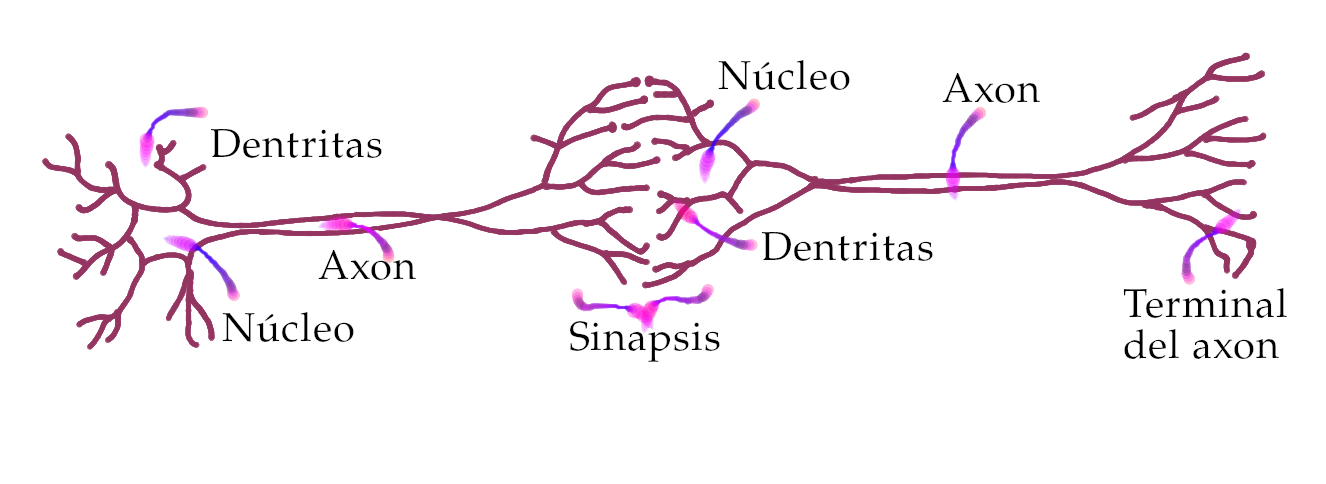
\includegraphics[width=0.75\textwidth]{/home/jessica/Tesis/img/tesis/BioloNN.png}
  \caption{Neuronas biológicas transmitiendo información \cite{Gardell:2010}}
  \label{fig:biologicalnn}
\end{figure}


\section{Arquitectura básica}

\subsection{El Perceptrón}\label{sec:perceptron}

La \autoref{fig:perceptron} muestra un diagrama de un modelo de Perceptrón, que es el modelo más simple de las \acp{ANN}. En este ejemplo la \textbf{capa de entrada} tiene dos componentes:
$$(x_1,x_2)$$
Es decir, $d=2$ en la \autoref{eq:trainset}. La constante $1$ es añadida para asignarle el \textbf{sesgo}: $b \in \mathbb{R}$, un parámetro que a menudo se emplea por razones de estadística. La \textbf{neurona} es la unidad computacional que calcula:

\begin{equation}
  \label{eq:neuronfun}
  f\left( \sum_{i=1}^dw_i\cdot x_i + b \right)
\end{equation}

donde los $w_i \in \mathbb{R}$ son conocidos como los \textbf{pesos} de $x_i$, y $f$ es una función \autoref{sec:FuncAct}.
\begin{figure}[hb]
  \centering
  \begin{tikzpicture}[x=1.5cm, y=1.5cm]
    % Input nodes
  \node[circle, draw, fill=CTtitle!30] (vac) at (0,1) {$1$};
  
  \node[circle, draw, fill=CTtitle!30] (input1) at (0,3) {$x_{1}$};
  \node[circle, draw, fill=CTtitle!30] (input2) at (0,2) {$x_{2}$};
    
    % Summation node
  \node[circle, draw, fill=CTtitle!60, minimum size=1.5cm] (sum) at (2,2) {$\Sigma / f(\Sigma)$};
  % Activation node
  %\node[circle, draw, fill=CTtitle!60, minimum size=1.5cm] (activation) at (4,2) {$f(\Sigma)$};
  % Output node
  \node[circle, draw, fill=CTtitle!30] (output) at (4,2) {$\hat{y}$};
  % Connect the nodes and add weights
  \foreach \i in {1,2}
  \draw[->] (input\i) -- node[midway, above] {$w_{\i}$} (sum);
  \draw[->] (vac) -- node[midway, above] {$b$} (sum);
  %\draw[->] (sum) -- (activation);
  \draw[->] (sum) -- (output);

  \node[above, yshift=2.5cm] at (0,2) {Entrada};
  \node[above, yshift=2.5cm] at (2,2) {Neurona};
  \node[above, yshift=2.5cm] at (4,2) {Salida};
  
\end{tikzpicture}

\caption{Diagrama de un modelo simple de Perceptrón}
\label{fig:perceptron}
\end{figure}

\marginpar{Para simplificar la lectura, en las siguientes secciones y capítulos se utilizará la palabra ``red'' para hacer referencia a la red neuronal artificial o \acs{ANN}.}El objetivo del algoritmo, es que mediante el entrenamiento de la red \autoref{sec:TrainNN} con un conjunto grande de $M$ datos: $\{\vec{x_j},y_j\}_{j=1}^{M}$ se obtengan los $w_i$ óptimos para que se cumpla:
$$y_l= \hat{y_l} = f\left( \sum_{i=1}^dw_i\cdot x_l \right)$$
con $y_l$ la etiqueta, o valor esperado, correspondiente al vector $\vec{x_l}$, en donde $(\vec{x_l},y_l)$ es un dato que no necesariamente pertenece al conjunto de entrenamiento que utilizó la red. Esta última propiedad es llamada \textbf{generalización del modelo}, y es lo que permite hacer predicciones sobre nuevos datos.

\subsection{Función de Activación}\label{sec:FuncAct}

En la \autoref{eq:neuronfun} la función $f$ es conocida como una \textbf{función de activación}. Algunos ejemplos de funciones de activación comúnmente utilizadas se muestran en la \autoref{fig:examplesfuncact}. 

\begin{figure}[htbp]
\centering

\subfloat[$y=Tanh(x)$]{%
\begin{tikzpicture}[scale=0.7]
\begin{axis}[
    xmin=-4.5, xmax=4.5,
    ymin=-1.2, ymax=1.2,
    axis lines=middle,
    xtick={-4,-3,...,4},
    ytick={-1,-0.5,0.5,1},
    ticklabel style={font=\tiny},
    samples=200,
    domain=-4.5:4.5,
    every axis plot post/.append style={line width=1pt}
]
\addplot[CTurl] {tanh(x)};
\end{axis}
\end{tikzpicture}
\label{fig:tanh}
}
\hfill
\subfloat[$y=x$]{%
\begin{tikzpicture}[scale=0.7]
\begin{axis}[
    xmin=-4.5, xmax=4.5,
    ymin=-4.5, ymax=4.5,
    axis lines=middle,
    xtick={-4,-3,...,4},
    ytick={-4,-3,...,4},
    ticklabel style={font=\tiny},
    samples=200,
    domain=-4.5:4.5,
    every axis plot post/.append style={line width=1pt}
]
\addplot[CTurl] {x};
\end{axis}
\end{tikzpicture}
\label{fig:identity}
}

\subfloat[$y=ReLU$]{%
\begin{tikzpicture}[scale=0.7]
\begin{axis}[
    xmin=-4.5, xmax=4.5,
    ymin=-4.5, ymax=4.5,
    axis lines=middle,
    xtick={-4,-3,...,4},
    ytick={-4,-3,...,4},
    ticklabel style={font=\tiny},
    samples=200,
    domain=-4.5:4.5,
    every axis plot post/.append style={line width=1pt}
]
\addplot[CTurl] {max(0,x)};
\end{axis}
\end{tikzpicture}
\label{fig:ReLU}
}
\hfill
\subfloat[$y=Sign$]{%
\begin{tikzpicture}[scale=0.7]
\begin{axis}[
    xmin=-4.5, xmax=4.5,
    ymin=-4.5, ymax=4.5,
    axis lines=middle,
    xtick={-4,-3,...,4},
    ytick={-4,-3,...,41},
    ticklabel style={font=\tiny},
    samples=200,
    domain=-4.5:4.5,
    every axis plot post/.append style={line width=1pt}
]
\addplot[CTurl] {sign(x)};
\end{axis}
\end{tikzpicture}
\label{fig:sign}
}
\caption{Ejemplos de funciones de activación}
\label{fig:examplesfuncact}
\end{figure}

La importancia en la elección de una función de activación u otra es más notable en los siguientes casos:
\begin{enumerate}
\item En la capa de salida de cualquier modelo de red
\item En los modelos multicapa \autoref{sec:multicapamodels}
\end{enumerate}
En el primer caso, la función de activación está motivada por el tipo de valores que puede tomar la etiqueta $y$. En problemas de clasificación binaria, las funciones de activación comúnmente utilizadas son \emph{Tanh} o \emph{Sigmoid}, en problemas de clasificación múltiple la función $Softmax$; cuando $y$ toma valores reales la función de activación utilizada es la \emph{Identidad} \autoref{fig:identity}.
\\
En el segundo caso, la importancia de elegir una función de activación no lineal entre capas para modelos de clasificación, por ejemplo, permite que el modelo pueda transformar un problema que inicialmente no es linealmente separable, a uno que sí lo es.


\subsection{Función de Pérdida}
La \textbf{función de pérdida}, o \textbf{loss function} en inglés: $L(\hat{y},y)$ es la función que compara el resultado o salida de la red: $\hat{y}$ respecto a la etiqueta original $y$ correspondiente a la entrada $\vec{x}$, en otras palabras, indica qué tan bueno es el modelo implementado. El modelo es mejor cuanto menos sea la diferencia entre el valor predicho $\hat{y}$ respecto al valor esperado $y$.
\\
En el entrenamiento de una red, el objetivo es minimizar esta función a través de la actualización de los pesos $w_i$. La elección de la función de pérdida, depende del problema a resolver, como en el caso de la función de activación de la última capa. Para modelos en donde los valores de la salida $\hat{y}$ son reales, se puede utilizar una \emph{Función de Pérdida Cuadrática} o \emph{Mean Square Error (MSE)} en inglés:
\begin{equation}
  \label{eq:MSE}
  L = (\hat{y}-y)^2
\end{equation}

Para problema de clasificación binaria se puede utilizar:
\begin{equation}
  \label{eq:bin}
  L = log(1 + \exp(−y\cdot \hat{y}))
\end{equation}

mientras que para problemas de múltiples categorías, donde $\hat{y}=(\hat{y}_1, ..., \hat{y}_k)$ son las probabilidades\footnote{Las probabilidades de cada clase se pueden obtener aplicando la función de activación \emph{softmax}.} de las $k$ clases\footnote{Las \textbf{clases} se refieren a las diferentes opciones de salida que puede tener una red de un problema de clasificación múltiple, por ejemplo si la red reconoce tres tipos de fruta, cada fruta es una clase distinta.} una función de pérdida que se puede aplicar es:
\begin{equation}
  \label{eq:otro}
  L = −log(\hat{y}_r)
\end{equation}
con $r$ la clase a la que corresponde la etiqueta $y$.

\subsection{Modelos Multicapa}\label{sec:multicapamodels}
En la sección \autoref{sec:perceptron} se revisó el Perceptrón como el modelo de red más simple. La \autoref{fig:nnlayers} muestra un diagrama de un modelo multicapa, estos modelos tienen capas ocultas entre las capas de entrada y salida, cada capa contiene un número determinado de neuronas o nodos. El número de capas ocultas y los nodos en cada una, son \textbf{hiper-parámetros} de la red, y en general\footnote{\emph{Hyperparameter Grid Search} es un método que se puede utilizar para conocer los hiper-parámetros óptimos de un modelo en particular, sin embargo, este proceso generalmente implica costos computacionales mayores.}, no se tiene una manera determinista para conocer los valores óptimos en cada modelo.

\begin{figure}[ht]
    \centering
    \begin{tikzpicture}[scale=1.5]
    
    % Input layer
    \foreach \i in {1,...,4}
        \node[circle, draw=black, fill=CTtitle!30] (I-\i) at (0,\i-2) {$x_{\i}$};
    
    % Hidden layer 1
    \foreach \i in {1,...,3}
        \node[circle, draw=black, fill=CTtitle!60] (H1-\i) at (2,\i-1.5) {};
    
    % Hidden layer 2
    \foreach \i in {1,...,3}
        \node[circle, draw=black, fill=CTtitle!60] (H2-\i) at (4,\i-1.5) {};
        
    % Output layer
    \foreach \i in {1,...,2}
        \node[circle, draw=black, fill=CTtitle!30] (O-\i) at (6,\i-1) {$y_{\i}$};
    
    % Connections
    \foreach \i in {1,...,4}
        \foreach \j in {1,...,3}
            \draw[->] (I-\i) -- (H1-\j);
            
    \foreach \i in {1,...,3}
        \foreach \j in {1,...,3}
            \draw[->] (H1-\i) -- (H2-\j);
            
    \foreach \i in {1,...,3}
        \foreach \j in {1,...,2}
            \draw[->] (H2-\i) -- (O-\j);
    
    % Labels
    \node[above, yshift=0.5cm] at (0,2) {Capa de Entrada};
    \node[above, yshift=0.5cm] at (2,2) {Capa oculta 1};
    \node[above, yshift=0.5cm] at (4,2) {Capa oculta 2};
    \node[above, yshift=0.5cm] at (6,2) {Capa de Salida};
    
    \end{tikzpicture}
    \caption{Diagrama de un modelo de \acs{ANN} Multicapa con dos capas ocultas.}
    \label{fig:nnlayers}
\end{figure}

La arquitectura específica de las redes multicapa se conoce como redes \emph{feed-forward}, pues las capas se alimentan una tras otra desde la capa de entrada hasta la capa de salida. La arquitectura por defecto de las redes feed-forward supone que todos los nodos de una capa están conectados a los de la capa siguiente. \cite{Nielsen:2018}
\\
La operación que realiza una red multicapa de la capa de entrada a la primer capa oculta con $p_1$ nodos está definida como:
$$\vec{h}_1 = f(W^T_1 \cdot \vec{x})$$
onde $W^T_1$ es la transpuesta de $W_1$, de dimensión $p_1 \times d$, y $\vec{x}$ el vector de entrada de dimensión $d$. La operación que se realiza de la capa oculta $p$ y la $p+1$ $\forall p \in \{1,...,k-1\}$ es:
$$\vec{h}_{p+1} = f(W^T_{p} \cdot \vec{h}_p)$$
donde $W^T_{p}$ es de dimensión $p_{r+1} \times p_r$ y $\vec{h}_p$ es de dimensión $p$. Finalmente, de la última capa oculta a la capa de salida con dimensión $o$ la operación realizada es:
$$\vec{o} = f(W^T_{k+1} \cdot \vec{h}_k)$$
con $W^T_{k+1}$ de dimensión $o \times p_{k}$, y $\vec{h}_k$ de dimensión $p_k$. En todas las expresiones $f$ es una función de activación que se aplica a cada elemento del vector.

\section{Entrenamiento de una Red Neuronal}\label{sec:TrainNN}
Una vez construida la arquitectura de una red, el objetivo es obtener los parámetros $w$ y $b$ de cada nodo y en cada capa, que minimicen la función de pérdida $L$. El algoritmo que se utiliza para minimizar la función de pérdida es conocido como \textbf{Descenso del Gradiente Estocástico}\footnote{poner algo del Descenso de Gradiente} o SGD por sus siglas en inglés. La \autoref{fig:gd} muestra un sencillo ejemplo del funcionamiento del algoritmo, en donde la función de pérdida únicamente depende de un parámetro $w$, el peso inicial es un valor aleatorio $w_1$, luego se calcula el valor del gradiente (en este caso unidimensional, la derivada) y se actualiza el peso como:
$$w_2 = w_1 - \alpha \frac{dL}{dw}\bigg|_{w_1}$$x
en donde $\alpha$ es un hiper-parámetro de la red llamado \textbf{tasa de aprendizaje} o \textbf{learning rate} en inglés. El proceso continúa actualizando $w$ hasta llegar a $w_m$, el mínimo de la función de pérdida, pues el algoritmo actualiza los pesos en dirección opuesta al gradiente, que apunta a la dirección de máximo cambio.

\begin{figure}[h]
  \centering
  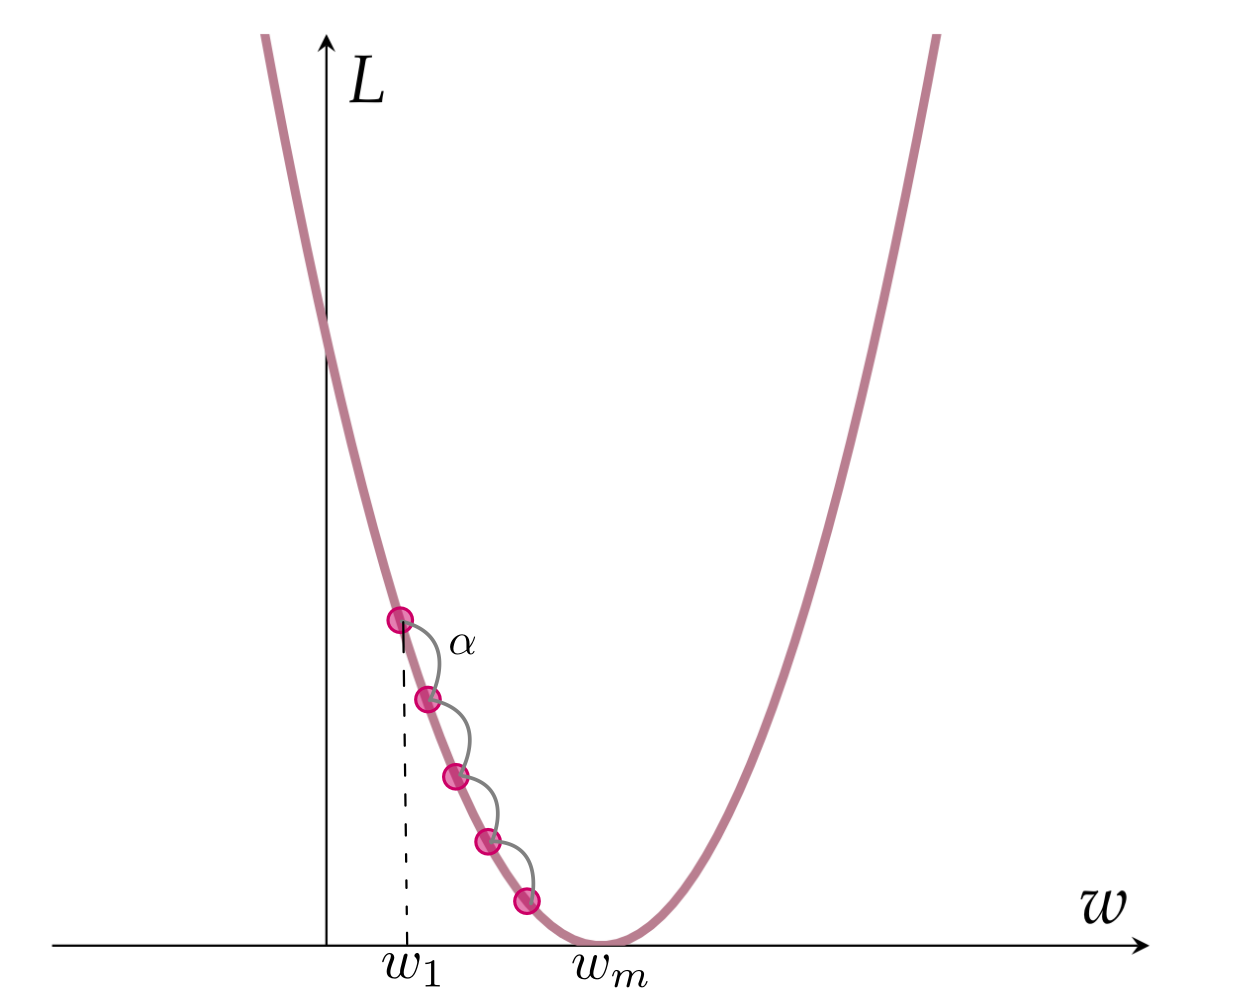
\includegraphics[width=0.7\textwidth]{/home/jessica/Tesis/img/tesis/GD.png}
\caption{Algoritmo de Descenso del Gradiente para una función de pérdida $L(w)$}
\label{fig:gd}
\end{figure}

Para modelos de una capa el proceso del Descenso del Gradiente es directo, pues la función de pérdida depende de los pesos de la
única capa, sin embargo, para modelos multicapa la función de pérdida es el resultado de una composición de múltiples funciones de los pesos de las capas anteriores, el algoritmo utilizado para calcular el gradiente en función de la composición se llama \textbf{Retropropagación} o \textbf{Backpropagation} en inglés, que se compone de dos fases principales:
\begin{enumerate}
\item Fase de avance: La red recibe las entradas con pesos establecidos de manera aleatoria, se calcula la función de pérdida y las derivadas respecto a la última capa, es decir, la capa de salida.
  \item Fase hacia atrás: En esta fase el objetivo es conocer el gradiente de la función de pérdida respecto a los pesos de las capas anteriores utilizando la regla de la cadena.
\end{enumerate}

La \autoref{fig:backprop} muestra un ejemplo de la composición de funciones que se realizan en una red neuronal. En este ejemplo existen se muestran dos capas antes de la salida $o$.

\begin{figure}[h]
  \centering
  \begin{tikzpicture}[scale=0.7,x=2cm,y=2cm]
  \node[draw, circle, fill=CTtitle!30, minimum size=1.5cm] (x1) at (0,0) {$f(w)$};
  \node[draw, circle, fill=CTtitle!30, minimum size=1.5cm] (h1) at (2,1) {$g(y)$};
  \node[draw, circle, fill=CTtitle!30, minimum size=1.5cm] (h2) at (2,-1) {$h(z)$};
  \node[draw, circle, fill=CTtitle!30, minimum size=1.5cm] (y) at (4,0) {$K(p,q)$};
  
  \draw[->] (-1,0) -- (x1)node[midway, above left] {$w$};
  \draw[->] (x1) -- (h1) node[midway, above left] {$y=f(w)$};
  \draw[->] (x1) -- (h2) node[midway, below left] {$z=f(w)$};
  \draw[->] (h1) -- (y) node[midway, above right] {$p=g(y)$};
  \draw[->] (h2) -- (y) node[midway, below right] {$q=h(z)$};
  \draw[->] (y) -- (5,0) node[midway, above right] {$o=K(p,q)$};
\end{tikzpicture}
\caption{Gráfica computacional con dos posibles caminos \cite{Nielsen:2018}}
\label{fig:backprop}
\end{figure}

Utilizando la regla de la cadena para funciones de varias variables se puede determinar la derivada de $o$ respecto al peso $w$:

\begin{align}
  \label{eq:ugly}
\frac{\partial o}{\partial w} &= \frac{\partial o}{\partial p} \cdot \frac{\partial p}{\partial w} +  \frac{\partial o}{\partial q} \cdot \frac{\partial q}{\partial w}  \\ 
                              &=  \frac{\partial o}{\partial p}\cdot\frac{\partial p}{\partial y}\cdot\frac{\partial y}{\partial w} + \frac{\partial o}{\partial q}\cdot \frac{\partial q}{\partial z}\cdot \frac{\partial z}{\partial w}\\
                              &= \frac{\partial K(p,q)}{\partial p}\cdot g'(y)\cdot f'(w) + \frac{\partial K(p,q)}{\partial q}\cdot h'(z)\cdot f'(w)
\end{align}

En este ejemplo existen únicamente dos caminos posibles de $w$ a $o$. En la práctica, las redes neuronales multicapa contienen una gran cantidad de caminos posibles entre los pesos de cada capa hasta la salida. Si se considera una secuencia de capas ocultas: $h_1,...,h_k$ seguida de la capa de salida $o$ respecto a la cual se calcula la función de pérdida $L$. La parcial de la función de pérdida respecto al peso $w_{h_r, h_{r+1}}$ de la conexión de la capa $h_{r}$ a la capa $h_{r+1}$ es: \cite{Nielsen:2018}

\begin{equation}
  \label{eq:partialw}
  \frac{\partial L}{\partial w_{h_r, h_{r+1}}} = \frac{\partial L}{\partial o}\cdot \left( \sum_{(h_r,h_{r+1},...,h_k,o)\in \mathcal{P}}\frac{\partial o}{\partial h_k}\prod_{i=r}^{k-1}\frac{\partial h_{i+1}}{\partial h_i}\right) \frac{\partial h_r}{\partial w_{h_{r-1},h_r}}
\end{equation}

una vez conocidos los gradientes respecto a los pesos en las múltiples capas, se actualizan los valores $w$ con el objetivo de minimizar la función de pérdida, y así mejorar el modelo.\\
El número de datos de entrenamiento, es decir de pares: $(X_l,y_l)$, que pasan por la red antes de que se actualicen los pesos, se llama \textbf{tamaño de lote} o \textbf{batch size} en inglés. Una vez que todos los datos de entrenamiento han pasado por la red, se dice que ha pasado una \textbf{época} o \textbf{epoch} en inglés. Tanto el número de épocas, como el tamaño de lote son hiper-parámetros de la red.

%K(p,q)=K(g(f(w)),h(f(w)))

%\addtocontents{toc}{\protect\clearpage} % <--- just debug stuff, ignore

%x%************************************************
\chapter{Implementación de modelos}\label{ch:ImpModelos}
% ************************************************
\section{División de los datos}

\subsection{Datos de entrenamiento (Train)}

\subsection{Datos de Validación (Validation)}

\subsection{Datos de prueba (Test)}


\section{Función de activación}

\section{Funciones de pérdida y métricas}

\section{Optimizador}
%%************************************************
\chapter{Redes Neuronales Convolucionales}\label{ch:CNN}
% ************************************************

\section{Modelo}

\section{Principales aplicaciones}



%agregar a forma final \cleardoublepage
%\ctparttext{You can put some informational part preamble text here.}
\part{Implementación de un modelo de ANN como propagador en Dinámica Cuántica }\label{pt:Modelos}
%************************************************
\chapter{LSTM como propagador en Dinámica Cuántica}\label{ch:LSTMapplied}
% ************************************************
\section{Introducción}
En el capítulo anterior se desarrollaron conceptos básicos generales de las redes neuronales, actualmente existen diversos tipos de redes que se aplican a problemas comunes y que se distinguen por su arquitectura.
\\
En este capítulo se abordará un modelo particular de red llamado \emph{Long Short-Term Memory} (\acs{LSTM}, por sus siglas en inglés), que pertenece a un tipo de redes llamadas \emph{Redes Neuronales Recurrentes} (\acp{RNN}, por sus siglas en inglés). Este tipo de redes es comúnmente utilizada cuando los atributos en el conjunto de datos están relacionados entre sí, o guardan una dependencia.
\\\\
En la sección \autoref{sec:lstm} se desarrollará la arquitectura de las redes \acs{LSTM}, así como sus aplicaciones más comunes, haciendo énfasis a las series de tiempo, que son de particular interés en el presente trabajo, pues la evolución temporal de un paquete de onda puede tratarse como un problema de series de tiempo, encontrando así una manera de abordar el problema de propagar una onda en el tiempo utilizando una red \acs{LSTM}.
\\
En la sección \autoref{sec:Project} se implementará el modelo de \acs{LSTM} que servirá como propagador $\mathcal{U}$ en la ecuación de Schrödinger Dependiente del Tiempo (\autoref{eq:TDSE ket}) para los potenciales $V(r,t)$ revisados en la sección \autoref{sec:ProtonTransfer}.
\\
A lo largo de la sección se presentará el conjunto de datos de entrenamiento de la red, así como los parámetros del modelo del potencial que se utilizaron para su obtención; también se presentarán los hiper-parámetros empleados en la red. Finalmente, en la sección \autoref{sec:Resultados} se presentarán los resultados y predicciones obtenidas con del modelo.

\section{Redes Neuronales Recurrentes}\label{sec:RNN}
Como se mencionó anteriormente, las Redes Neuronales Recurrentes se emplean cuando entre los atributos del conjunto de datos existen relaciones. Un dato de entrada para este tipo de redes puede verse de la siguiente forma:

\begin{equation}
  \label{eq:xdataRNN}
  \vec{X} = (\vec{x}_0, \vec{x}_1, \dots , \vec{x}_n)
\end{equation}

en donde cada $\vec{x}_t$ es un vector de dimensión $d$ recibido al tiempo $t$. Para cada tiempo $t$ se tiene un valor de salida: $\vec{y}_t$ con la misma dimensión.
\\
Algunos ejemplos de aplicaciones se muestran a continuación:

\begin{itemize}[label=\textcolor{CTtitle}{\textbullet}]
\item \emph{Secuencias de texto:} En donde la importancia o información de una palabra depende del contexto en el que se encuentra dentro de una oración. Cada palabra\footnote{En este caso, la dimensión $d$ hace referencia al número de palabras que tiene el léxico utilizado.}: $\vec{x}_t$,  puede verse como un atributo relacionado a la palabra anterior en una oración: $\vec{x}_{t-1}$, o a la palabra siguiente: $\vec{x}_{t+1}$.
 \item \emph{Series de tiempo:} $\vec{x}_t$ en este caso puede almacenar $d$ valores, que pueden ser, por ejemplo, los correspondientes al valor de una función $f(x,t)$ en una maya de $d$ puntos en el espacio $x$ al tiempo $t$. En este tipo de configuración la salida $\vec{y}_t$ podría ser la predicción pronosticada de $\vec{x}_{t+1}$.
 \end{itemize}
  
Un diagrama sencillo de una \acs{RNN} se muestra en la \autoref{fig:RNN}, en donde un auto-bucle actualizará el \textbf{estado oculto} $\vec{h}_t$ a cada tiempo $t$ después de la entrada $\vec{x}_t$:
\begin{equation}
  \label{eq:hidden}
  \vec{h}_t = Tanh(W_{xh}\vec{x}_t + W_{hh} \vec{h}_{t-1})
\end{equation}
%\begin{equation}
%  \vec{h}_t = f(\vec{h}_{t-1}, \vec{x}_t)
%\end{equation}
donde $Tanh$ es la función de activación, que está siendo aplicada a cada elemento del vector resultante de la multiplicación y suma de las matrices de peso $W$ por los vectores $\vec{x}_t$ y $\vec{h}_{t-1}$ para cada tiempo $t$. La salida, por su parte, está dada por:
\begin{equation}
  \vec{y}_t = W_{hy}\vec{h}_t
\end{equation}

\begin{figure}[!htbp]
  \centering
  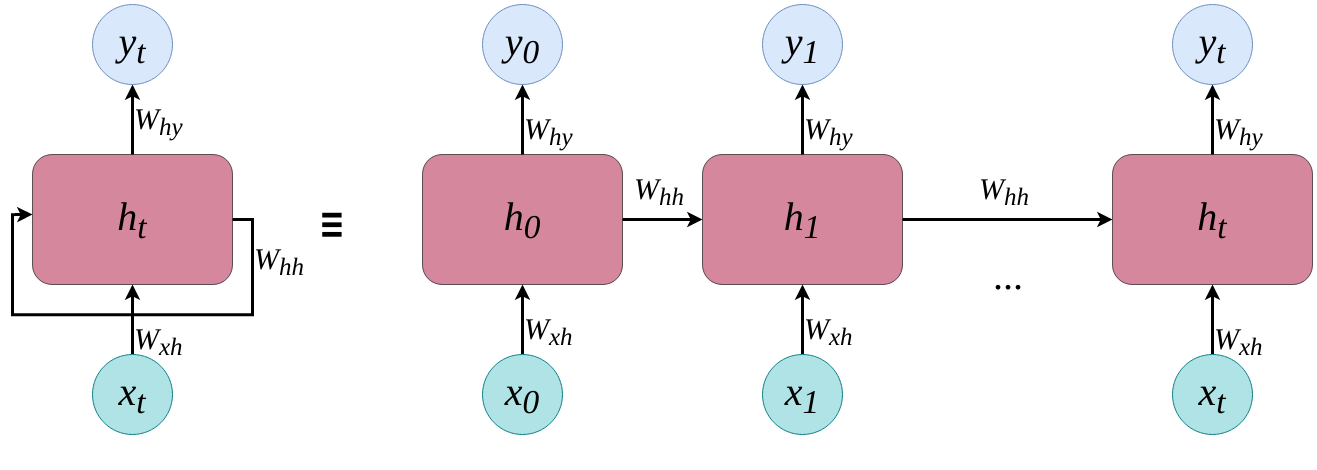
\includegraphics[width=0.9\textwidth]{/home/jessica/Tesis/img/tesis/RNN.png}
  \caption{Diagrama de una \acs{RNN} y su representación en capas de tiempo.}
  \label{fig:RNN}
\end{figure}

En la \autoref{fig:RNN}, a la derecha se muestra la representación de la \acs{RNN} en capas para cada tiempo, en donde es importante notar que las matrices de peso $W$ son las mismas en cada tiempo $t$, de manera que ecuación de recurrencia \autoref{eq:hidden} aplica la misma función.
\\

Uno de los principales problemas de las \acp{RNN} en la práctica es en el entrenamiento, pues el gradiente tiende a desvanecerse o incrementar excesivamente, debido a la inestabilidad que produce la multiplicación de forma recursiva de las matrices de peso $W$, problema que puede incrementarse cuanto más grande sea la secuencia de tiempo que procesa la red y cuantas más capas ocultas tenga.
\\
Una alternativa que previene este problema es el cambio de la relación de recurrencia para el estado oculto $\vec{h}_t$ (\autoref{eq:hidden}) mediante el uso de la \emph{memoria a largo plazo} de una red \acs{LSTM}, que se abordará en la siguiente sección. \cite{Nielsen:2018}

\section{Redes Long-Short Term Memory}\label{sec:lstm}

Las redes Long-Short Term Memory son un tipo de \acs{RNN} diseñadas para mitigar los problemas con el gradiente que estas tienen en el entrenamiento. La manera en la que realizan esto es cambiando las condiciones de recurrencia de cómo el estado oculto $\vec{h}_t$ es propagado en el tiempo, para ello, se introduce un nuevo vector llamado \textbf{celda de estado}: $\vec{c}_{t}$ de la misma dimensión de $\vec{h}_t$, que puede interpretarse como una \emph{memoria a largo plazo} que retiene parte de la información de las celdas de estados de tiempos pasados. \cite{Nielsen:2018}

\begin{figure}[!htbp]
  \centering
  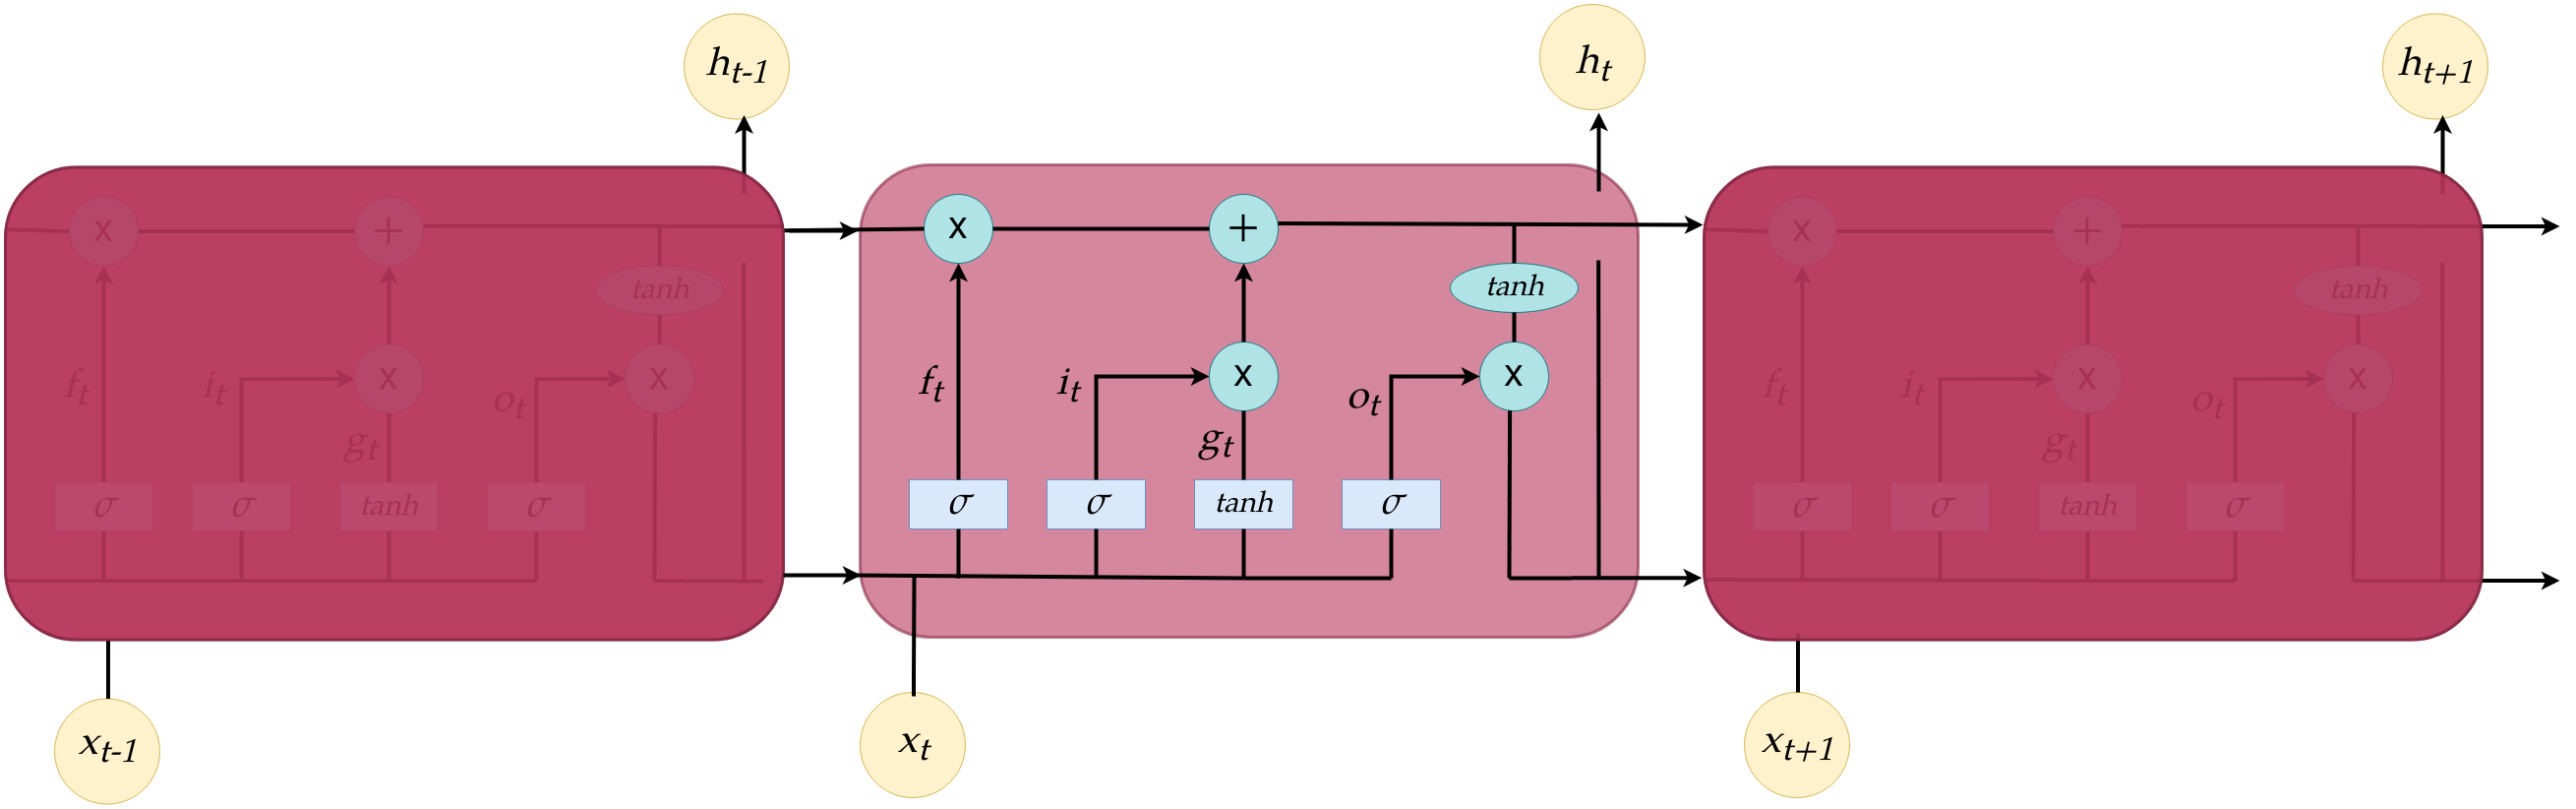
\includegraphics[width=0.9\textwidth]{/home/jessica/Tesis/img/tesis/LSTM_layerS.drawio.png}
  \caption{Diagrama de una \acs{LSTM} representada en capas de tiempo.}
  \label{fig:LSTMlayerS}
\end{figure}

El diagrama de la \autoref{fig:LSTMlayerS} muestra la estructura de una \acs{LSTM} desplegada en capas de tiempo, su forma en cadena es igual a la de las \acp{RNN} mencionadas en la sección anterior, sin embargo, cada bloque de memoria (recuadros rosas) tiene una arquitectura particular más compleja que la de una \acs{RNN} común.

\subsection{Arquitectura}\label{sec:LSTM_Arch}
La \autoref{fig:LSTMlayer} muestra un bloque de memoria de una \acs{LSTM}, en donde se observa cómo interactúan los vectores de estado oculto y de celda de estado pasados: $\vec{h}_{t-1}$ y $\vec{c}_{t-1}$ con funciones llamadas compuertas: $\vec{f}_t$, $\vec{i}_t$, $\vec{o}_t$ y operaciones básicas como suma y multiplicación, para producir nuevos vectores $\vec{h}_{t}$ y $\vec{c}_{t}$. Al tiempo $t=0$, los vectores de estado oculto y de celda de estado comienzan inicializados con un valor aleatorio.

\begin{figure}[!htbp]
  \centering
  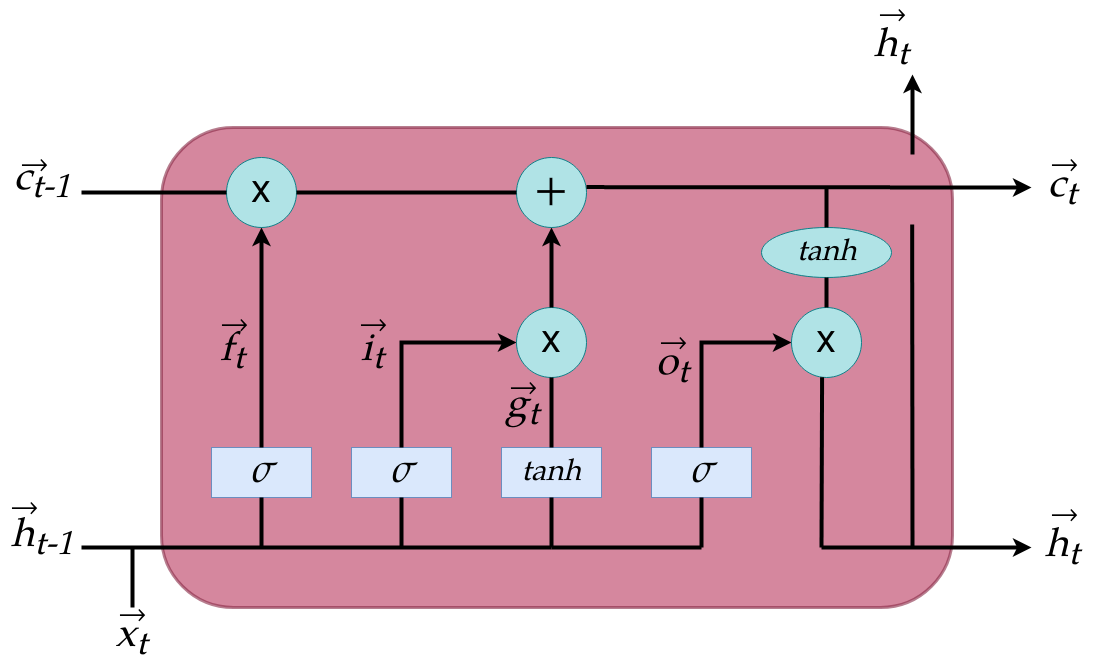
\includegraphics[width=0.7\textwidth]{/home/jessica/Tesis/img/tesis/LSTM_layer.png}
  \caption{Diagrama de un Bloque de Memoria de una \acs{LSTM}.}
  \label{fig:LSTMlayer}
\end{figure}

Una compuerta llamada \textbf{forget} $\vec{f}$, decide qué información proveniente del tiempo anterior: $t-1$ se mantiene y cual no, tomando en consideración también la entrada $\vec{x}_t$, aplicando la función $\sigma$ (es decir, $\vec{f}$ es una capa \emph{Sigmoid}):

\begin{equation}\label{eq:ft}
\vec{f}_t = \sigma(W_{xf}\vec{x}_t + W_{hf}\vec{h}_{t-1} + b_f)
\end{equation}

En donde $W$ y $b$ con sus correspondientes subíndices representan las matrices de peso y vectores de sesgo correspondientes a cada capa oculta. \\
Posteriormente, para decidir qué nueva información será incluida a la celda de estado se calculan:

\begin{equation}\label{eq:it}
\vec{i}_t = \sigma(W_{xi}\vec{x}_t + W_{hi}\vec{h}_{t-1} + b_i)
\end{equation}
\begin{equation}
  \label{eq:gt}
\vec{g}_t = Tanh(W_{xg}\vec{x}_t + W_{hg}\vec{h}_{t-1} + b_g)  
\end{equation}

en donde $\vec{i}$ es una capa \emph{Sigmoid}, llamada compuerta \textbf{input}, y $\vec{g}$ es una capa \emph{Tanh} que genera un vector con valores nuevos que son candidatos para ser agregados a la nueva celda de estado $\vec{c}_t$.
\\
La actualización de la celda de estado se da como:

\begin{equation}\label{eq:ct}
\vec{c}_t = \vec{f}_t \ast \vec{c}_{t-1} + \vec{i}_t \ast \vec{g}_t
\end{equation}

en donde $\ast$ representa el \emph{producto Hadamard}, en donde la multiplicación de los vectores se realiza elemento por elemento. Finalmente, la salida esta dada por:

\begin{equation}\label{eq:ot}
\vec{o}_t = \sigma(W_{xo}\vec{x}_t + W_{ho}\vec{h}_{t-1} + b_o)
\end{equation}

\begin{equation}\label{eq:ht}
\vec{h}_t = \vec{o}_t\ast Tanh(\vec{c}_t)
\end{equation}

en donde $\vec{o}$ es una capa \emph{Sigmoid} llamada compuerta \textbf{output}, y el vector $\vec{h}_t$ es el estado oculto al tiempo $t$, que servirá como entrada, junto con el vector de celda de estado $\vec{c}_t$ para el bloque de memoria del tiempo $t+1$, como se muestra en la \autoref{fig:LSTMlayerS}.

% ************************************************************
% ************************************************************
% PROYECTO
% ************************************************************
% ************************************************************

\section{Propagación temporal de Funciones de Onda con LSTM}\label{sec:Project}

En esta sección se implementa una red \acs{LSTM} para predecir la evolución temporal de un paquete de onda a un tiempo t $\psi(r,t)$ bajo un potencial dependiente del tiempo $V(r,t)$ después de un intervalo de tiempo $\Delta t$: $\psi(r,t+\Delta t)$. Tomando como referencia un trabajo previo \cite{Main:2021} en donde se implementó un modelo de perceptrón multicapa.

\subsection{Obtención de Datos}

El conjunto de datos de entrenamiento utilizado se obtuvo generando 4700 trayectorias de $200\,fs$, cada una con un $\Delta t = 1\,fs$. El diagrama de la \autoref{fig:DiagTraj} muestra una trayectoria, en donde $\psi(r,t_l)r$ con $l=0,\dots 200$ representa la parte real del paquete de onda, $\psi(r,t_l)i$ la parte imaginaria y $V(r,t_l)$ el potencial.

\begin{figure}[!htbp]
  \centering
  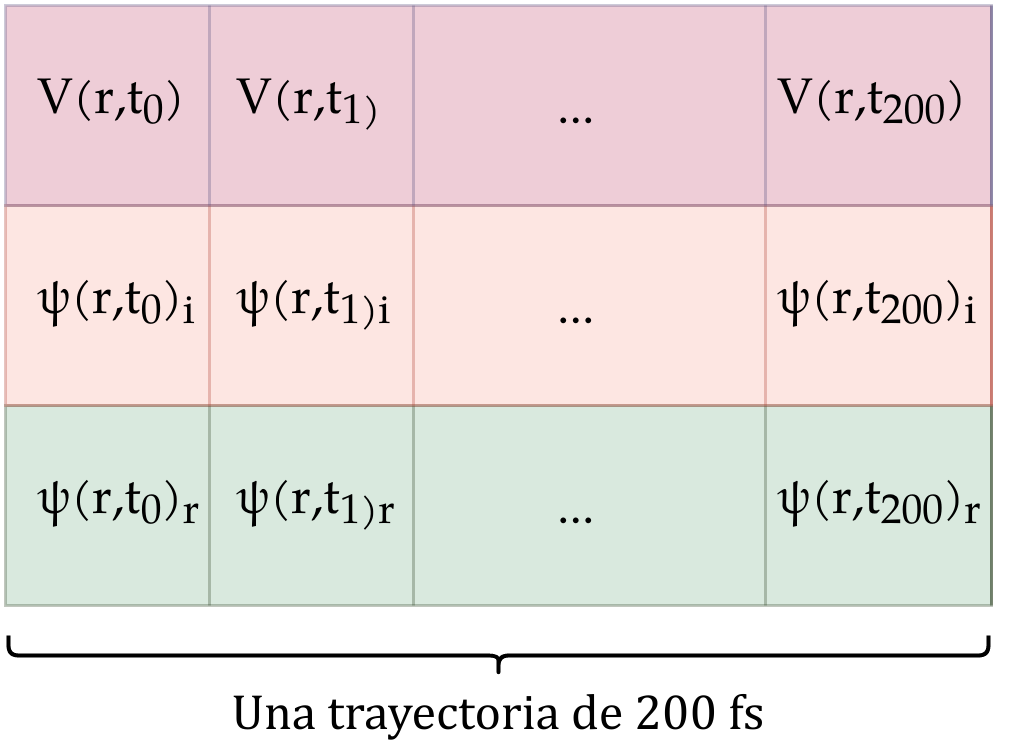
\includegraphics[width=0.7\textwidth]{/home/jessica/Tesis/img/tesis/DiagTrayectoria.png}
  \caption{Diagrama de una trayectoria generada.\\Para cada tiempo $t_i$ la onda $\psi(r,t_i)$ contiene el valor de la onda en los $N=32$ puntos en el grid del espacio de posiciones en $r$.}
  \label{fig:DiagTraj}
\end{figure}

Para cada trayectoria, los paquetes de onda iniciales, es decir al tiempo $t=0$, se definieron como ondas Gaussianas: (\autoref{fig:Gauss})
\begin{figure}[!htbp]
  \centering
  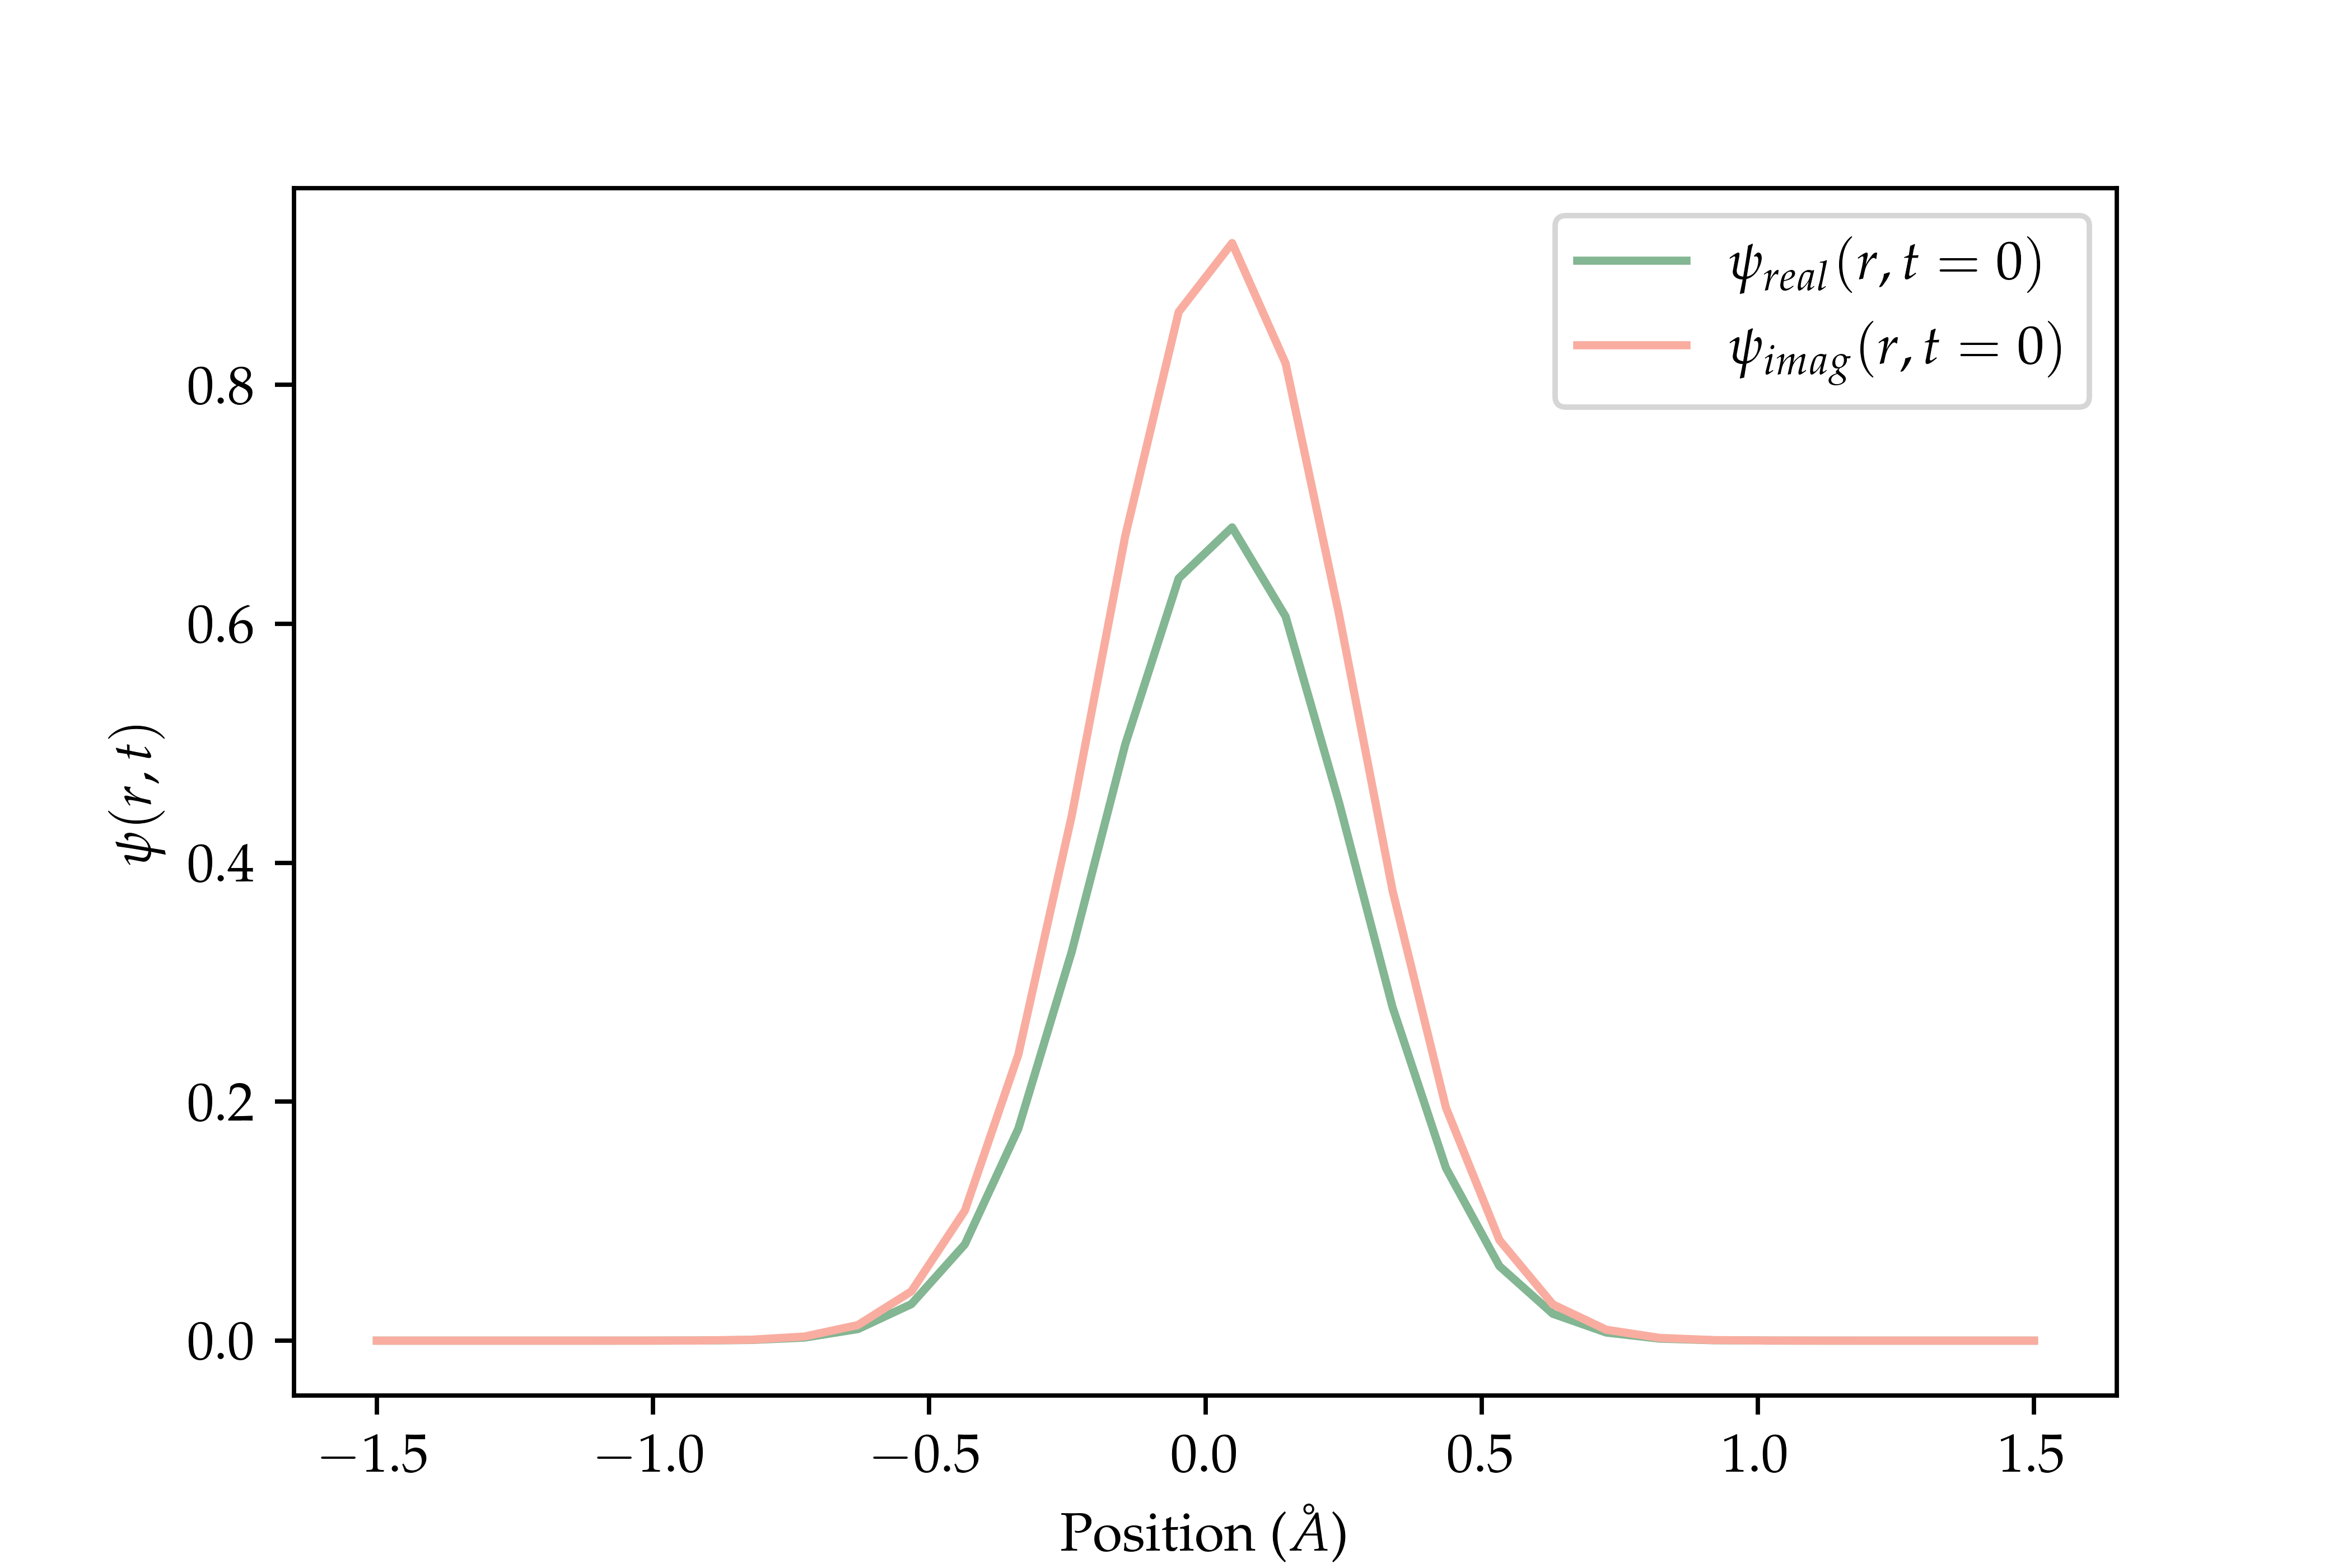
\includegraphics[width=1\textwidth]{/home/jessica/Tesis/img/tesis/DataWave.png}
  \caption{Parte real y compleja de un paquete de onda inicial $\psi(r,t=0)$.}
  \label{fig:Gauss}
\end{figure}

\begin{equation}
  \label{eq:gaussian}
  \psi(r,0) = C_i\cdot \frac{1}{\sigma\sqrt{2\pi}}\exp{\frac{-(r-\mu)^2}{2\sigma^2}}
\end{equation}
en donde $\mu$ y $\sigma$ son valores aleatorios elegidos de una distribución uniforme de $(-0.5,0.5)\mathring{A}$ y $(0.1,0.3)\mathring{A}$ respectivamente. $C_i$ es un número complejo aleatorio elegido de tal manera que la onda esté normalizada, es decir:
$$\bra{\psi(r,0)}\ket{\psi(r,0)} = 1$$

Para propagar la onda se utilizó el método \acs{DVR} revisado en la sección \autoref{sec:DVRapp} con un grid de $N=32$ puntos, con $a=r_0=-1.5\mathring{A}$ y $b=r_{N-1}=1.5\mathring{A}$ (\autoref{eq:grid}).
\\
El modelo de potencial $V(r,t)$ utilizado fue el mismo que se usó en la sección \autoref{sec:ProtonTransfer}. Para cada trayectoria se eligieron valores de parámetros para el modelo de potencial aleatorios entre rangos especificados en la \autoref{tab:RangeValuesPot}. En la \autoref{fig:Pote} se muestra un ejemplo de un potencial generado.
\begin{figure}[!htbp]
  \centering
  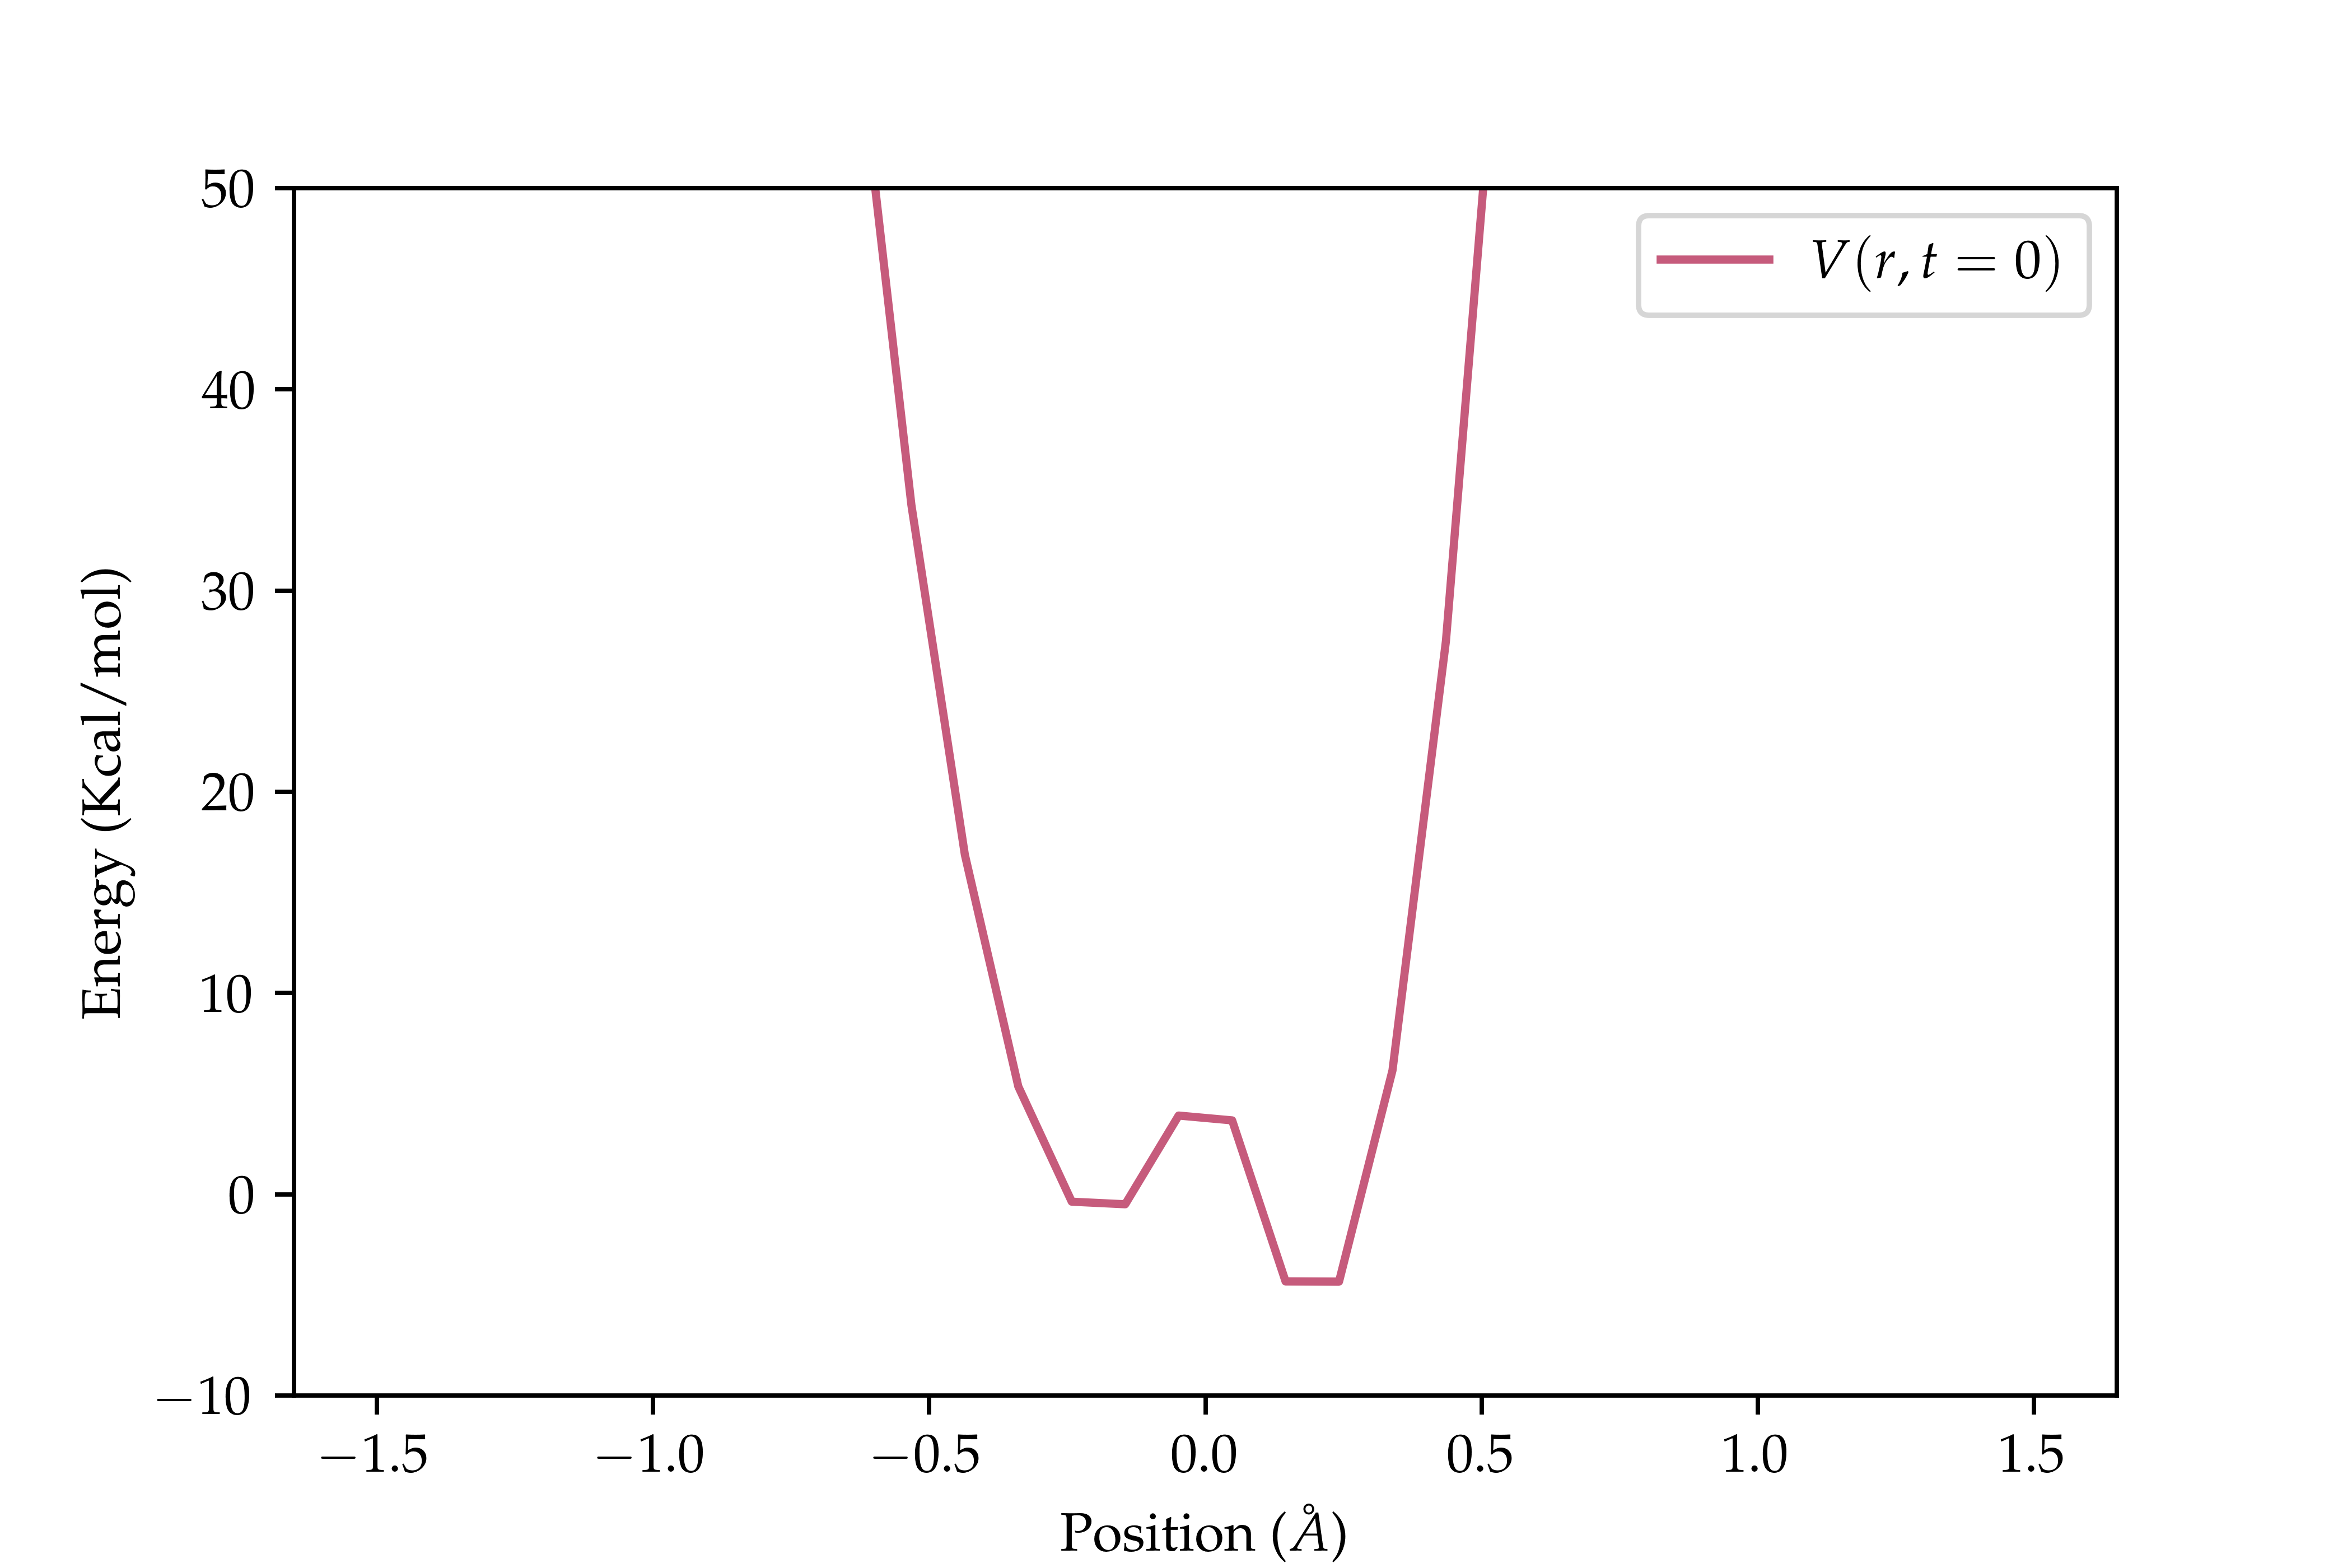
\includegraphics[width=1\textwidth]{/home/jessica/Tesis/img/tesis/DataPot.png}
  \caption{Potencial inicial al tiempo $t=0$}
  \label{fig:Pote}
\end{figure}

En el repositorio \href{https://github.com/Jessi-MM/PropagatorLearning/tree/main/Data_Gaussian}{\faGithub Trayectorias} se encuentran los datos generados. Cada carpeta contiene los directorios y archivos siguientes:

 \begin{forest}
      for tree={
        font=\ttfamily,
        grow'=0,
        math content,
        align=center,
        child anchor=west,
        parent anchor=south,
        anchor=west,
        calign=first,
        inner xsep=7pt,
        edge path={
          \noexpand\path [draw, \forestoption{edge}]
          (!u.south west) +(7.5pt,0) |- (.child anchor) pic {folder} \forestoption{edge label};
        },
        % style for your file node 
        file/.style={edge path={\noexpand\path [draw, \forestoption{edge}]
          (!u.south west) +(7.5pt,0) |- (.child anchor) \forestoption{edge label};},
          inner xsep=2pt,font=\small\ttfamily
                     },
        before typesetting nodes={
          if n=1
            {insert before={[,phantom]}}
            {}
        },
        fit=band,
        before computing xy={l=15pt},
      }  
    [Trayectorias
      [data0
      [Potential
      [0-Potential.npy\\$\vdots$,file]
      [200-Potential.npy,file
      ]
        ]
        [Wavepacket
        [0-Wavepacket.npy\\$\vdots$,file
        ]
        [200-Wavepacket.npy,file
        ]
        ]
      ]
    ]
 \end{forest}

 En donde \texttt{data0} corresponde a la trayectoria $0$. El archivo \emph{0-Potential.npy} es un arreglo de $N=32$ entradas que corresponde al valor del potencial al tiempo $t=0\,fs$, el archivo \emph{0-Wavepacket.npy} es un arreglo de $N=32$ entradas complejas que corresponden al paquete de onda al tiempo $t=0\,fs$; así respectivamente para cada tiempo hasta $t=200\,fs$. Además de los datos, se encuentra un archivo de texto: \emph{ValuesPotential.txt}, en donde se registran los valores de los parámetros para generar el potencial, es decir, los valores exactos elegidos de la \autoref{tab:RangeValuesPot}.
 \\
 
 El código para generar las trayectorias se encuentra en el repositorio: \href{https://github.com/Jessi-MM/PropagatorLearning/blob/main/src/Proton_Transfer_DataGenerate.ipynb}{\faGithub Generación de datos}, que contiene dos clases: \emph{Potential\_System}, que contiene las ecuaciones del modelo del potencial y la clase \emph{ProtonTransfer}, con la que se generan las trayectorias. A continuación se muestra un ejemplo para generar una trayectoria, con la información que muestra el diagrama de la \autoref{fig:DiagTraj}:

 \begin{lstlisting}
   trayectoria0 = ProtonTransfer(n=32, a=-1.5, b=1.5, time=True, var_random=True, save_dir='data0')
   trayectoria0.vector_potential(t=200,step=1)
   trayectoria0.evolution_wp(t=200, step=1, gaussiana=True)
\end{lstlisting}

En donde se utilizan las siguientes variables:
\begin{itemize}[label=\textcolor{CTtitle}{\textbullet}]
\item n: Número de puntos en el grid
\item a: Punto inicial del grid $[\mathring{A}]$
\item b: Punto final del grid $[\mathring{A}]$
\item time: True o False. Determina si se utiliza un potencial dependiente del tiempo: True, o independiente del tiempo: False  
\item var\_random: True o False. True inicia las variables de manera aleatoria para el potencial del sistema. False solicita al usuario cada variable. \autoref{tab:RangeValuesPot}
\item save\_dir: Nombre del directorio donde se guardarán los datos del potencial y la evolución de onda.
\item t: Tiempo total de la trayectoria $[fs]$
\item step: $\Delta t$ para la evolución temporal de la onda $[fs]$
\item gaussiana: True o False. True genera una onda inicial Gaussiana (\autoref{eq:gaussian}), False solicita $k$ para generar la onda inicial como una suma de eigenfunciones (\autoref{eq:psi_0}) 
\end{itemize}

\subsection{Procesamiento de Datos: Visualización y Forma}

Una vez generadas las trayectorias, para entrenar el modelo de red 


\begin{figure}[!htbp]
  \centering
  \includegraphics[width=0.5\textwidth]{/home/jessica/Tesis/img/tesis/InputOutput.png}
  \caption{Entrada $X$ y etiqueta $y$ a un tiempo $t$.}
  \label{fig:dataexample}
\end{figure}


blabla  a\footnote{Las funciones de onda $\psi$ están escaladas por un factor de 20 para poder visualizar el potencial en la misma gráfica.}

\begin{figure}[!htbp]
  \centering
  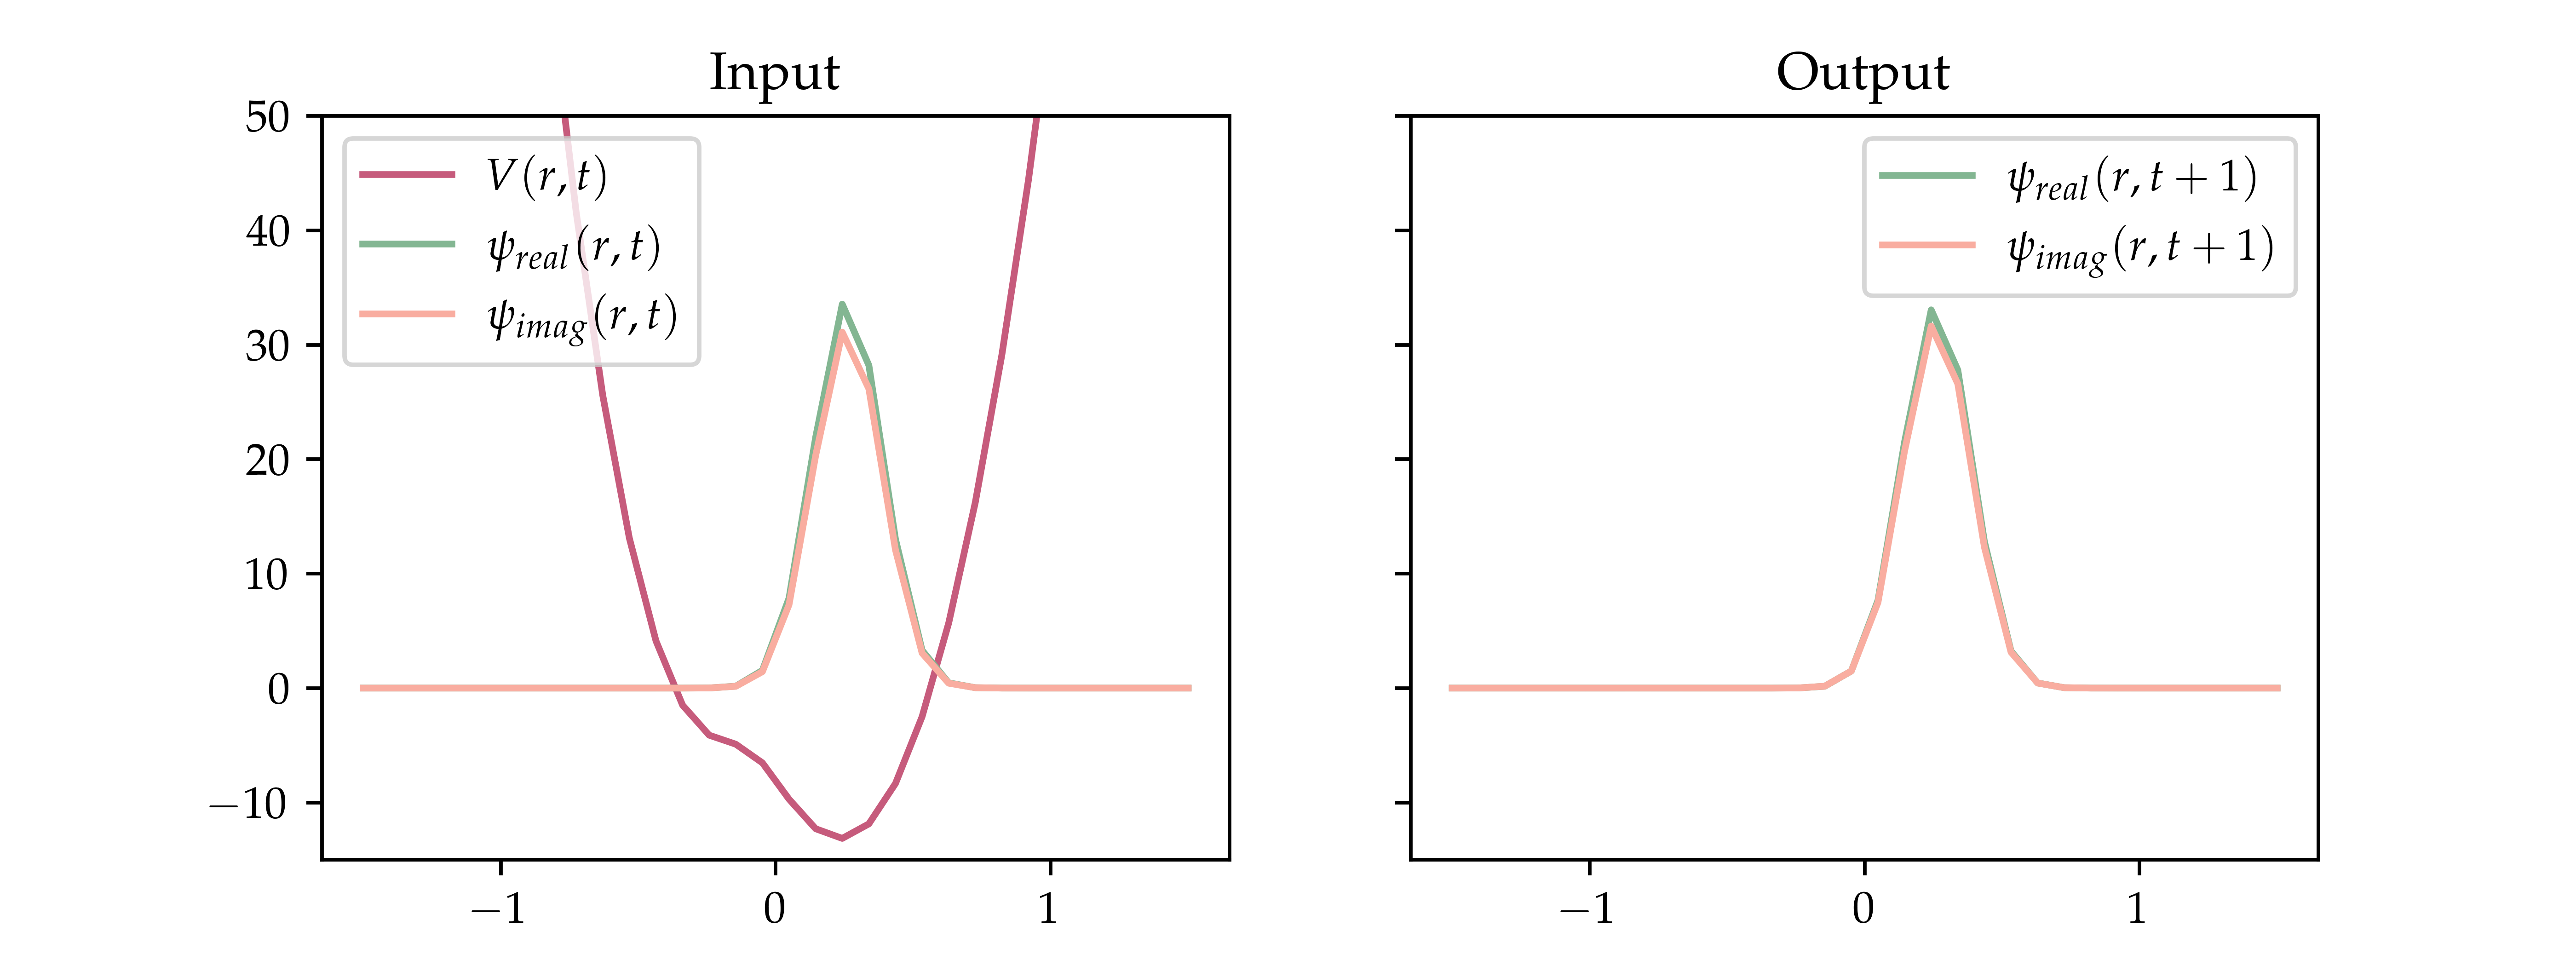
\includegraphics[width=0.8\textwidth]{/home/jessica/Tesis/img/tesis/dataInputOutput.png}
  \caption{Visualización: Entrada $X(t)$ y etiqueta $X^*(t+1)$ a un tiempo $t$.}
  \label{fig:datavis}
\end{figure}




\begin{figure}[!htbp]
  \centering
  \includegraphics[width=0.7\textwidth]{/home/jessica/Tesis/img/tesis/DiagramaSeqDatos.png}
  \caption{Vector $X$ a un tiempo $t$.}
  \label{fig:dataexamp}
\end{figure}


\begin{table}[ht]
  \myfloatalign
  \begin{tabularx}{0.7\textwidth}{XXXX} \toprule
   \tableheadline{Entrenamiento} & \tableheadline{Validación} & \tableheadline{Test} & \tableheadline{Total} \\ \midrule
   3290          &  940  & 470  & 4700  \\ \midrule
   70\%          &  20\% & 10\% & 100\% \\
    \bottomrule
  \end{tabularx}
  \caption{División de datos}
  \label{tab:SplitData}
\end{table}



\subsection{Modelo LSTM}

\begin{table}[ht]
  \myfloatalign
  \begin{tabularx}{\textwidth}{XXX} \toprule
   \tableheadline{Capas} & \tableheadline{Nodos} & \tableheadline{Entrada/Salida} \\ \midrule
   LSTM          &  1024  & (In: 96, Ou:1024)  \\ \midrule
   LSTM          &  1024  & (In: 1024, Ou:1024)  \\ \midrule
   Lineal        &  64    & (In: 1024, Ou:64) \\
    \bottomrule
  \end{tabularx}
  \caption{Resumen del modelo}
  \label{tab:model}
\end{table}

%\begin{figure}[!htbp]
 % \centering
  %\includegraphics[width=1\textwidth]{/home/jessica/Tesis/Codigo_Limpio/src/ANN_Models/img/LSTM_0-model.png}
  %\caption{Diagrama del modelo LSTM. Move to appendix ?}
 % \label{fig:modelDiag}
%\end{figure}

\subsection{Función de Precisión}

\begin{equation}
  \label{eq:S}
  S = \bra{\psi_{LSTM}}\ket{\psi_{True}} = |S|\exp{i\theta}
\end{equation}



\subsection{Resultados y Análisis: Precisión y Predicciones}\label{sec:Resultados}

\begin{figure}[!htbp]
  \centering
  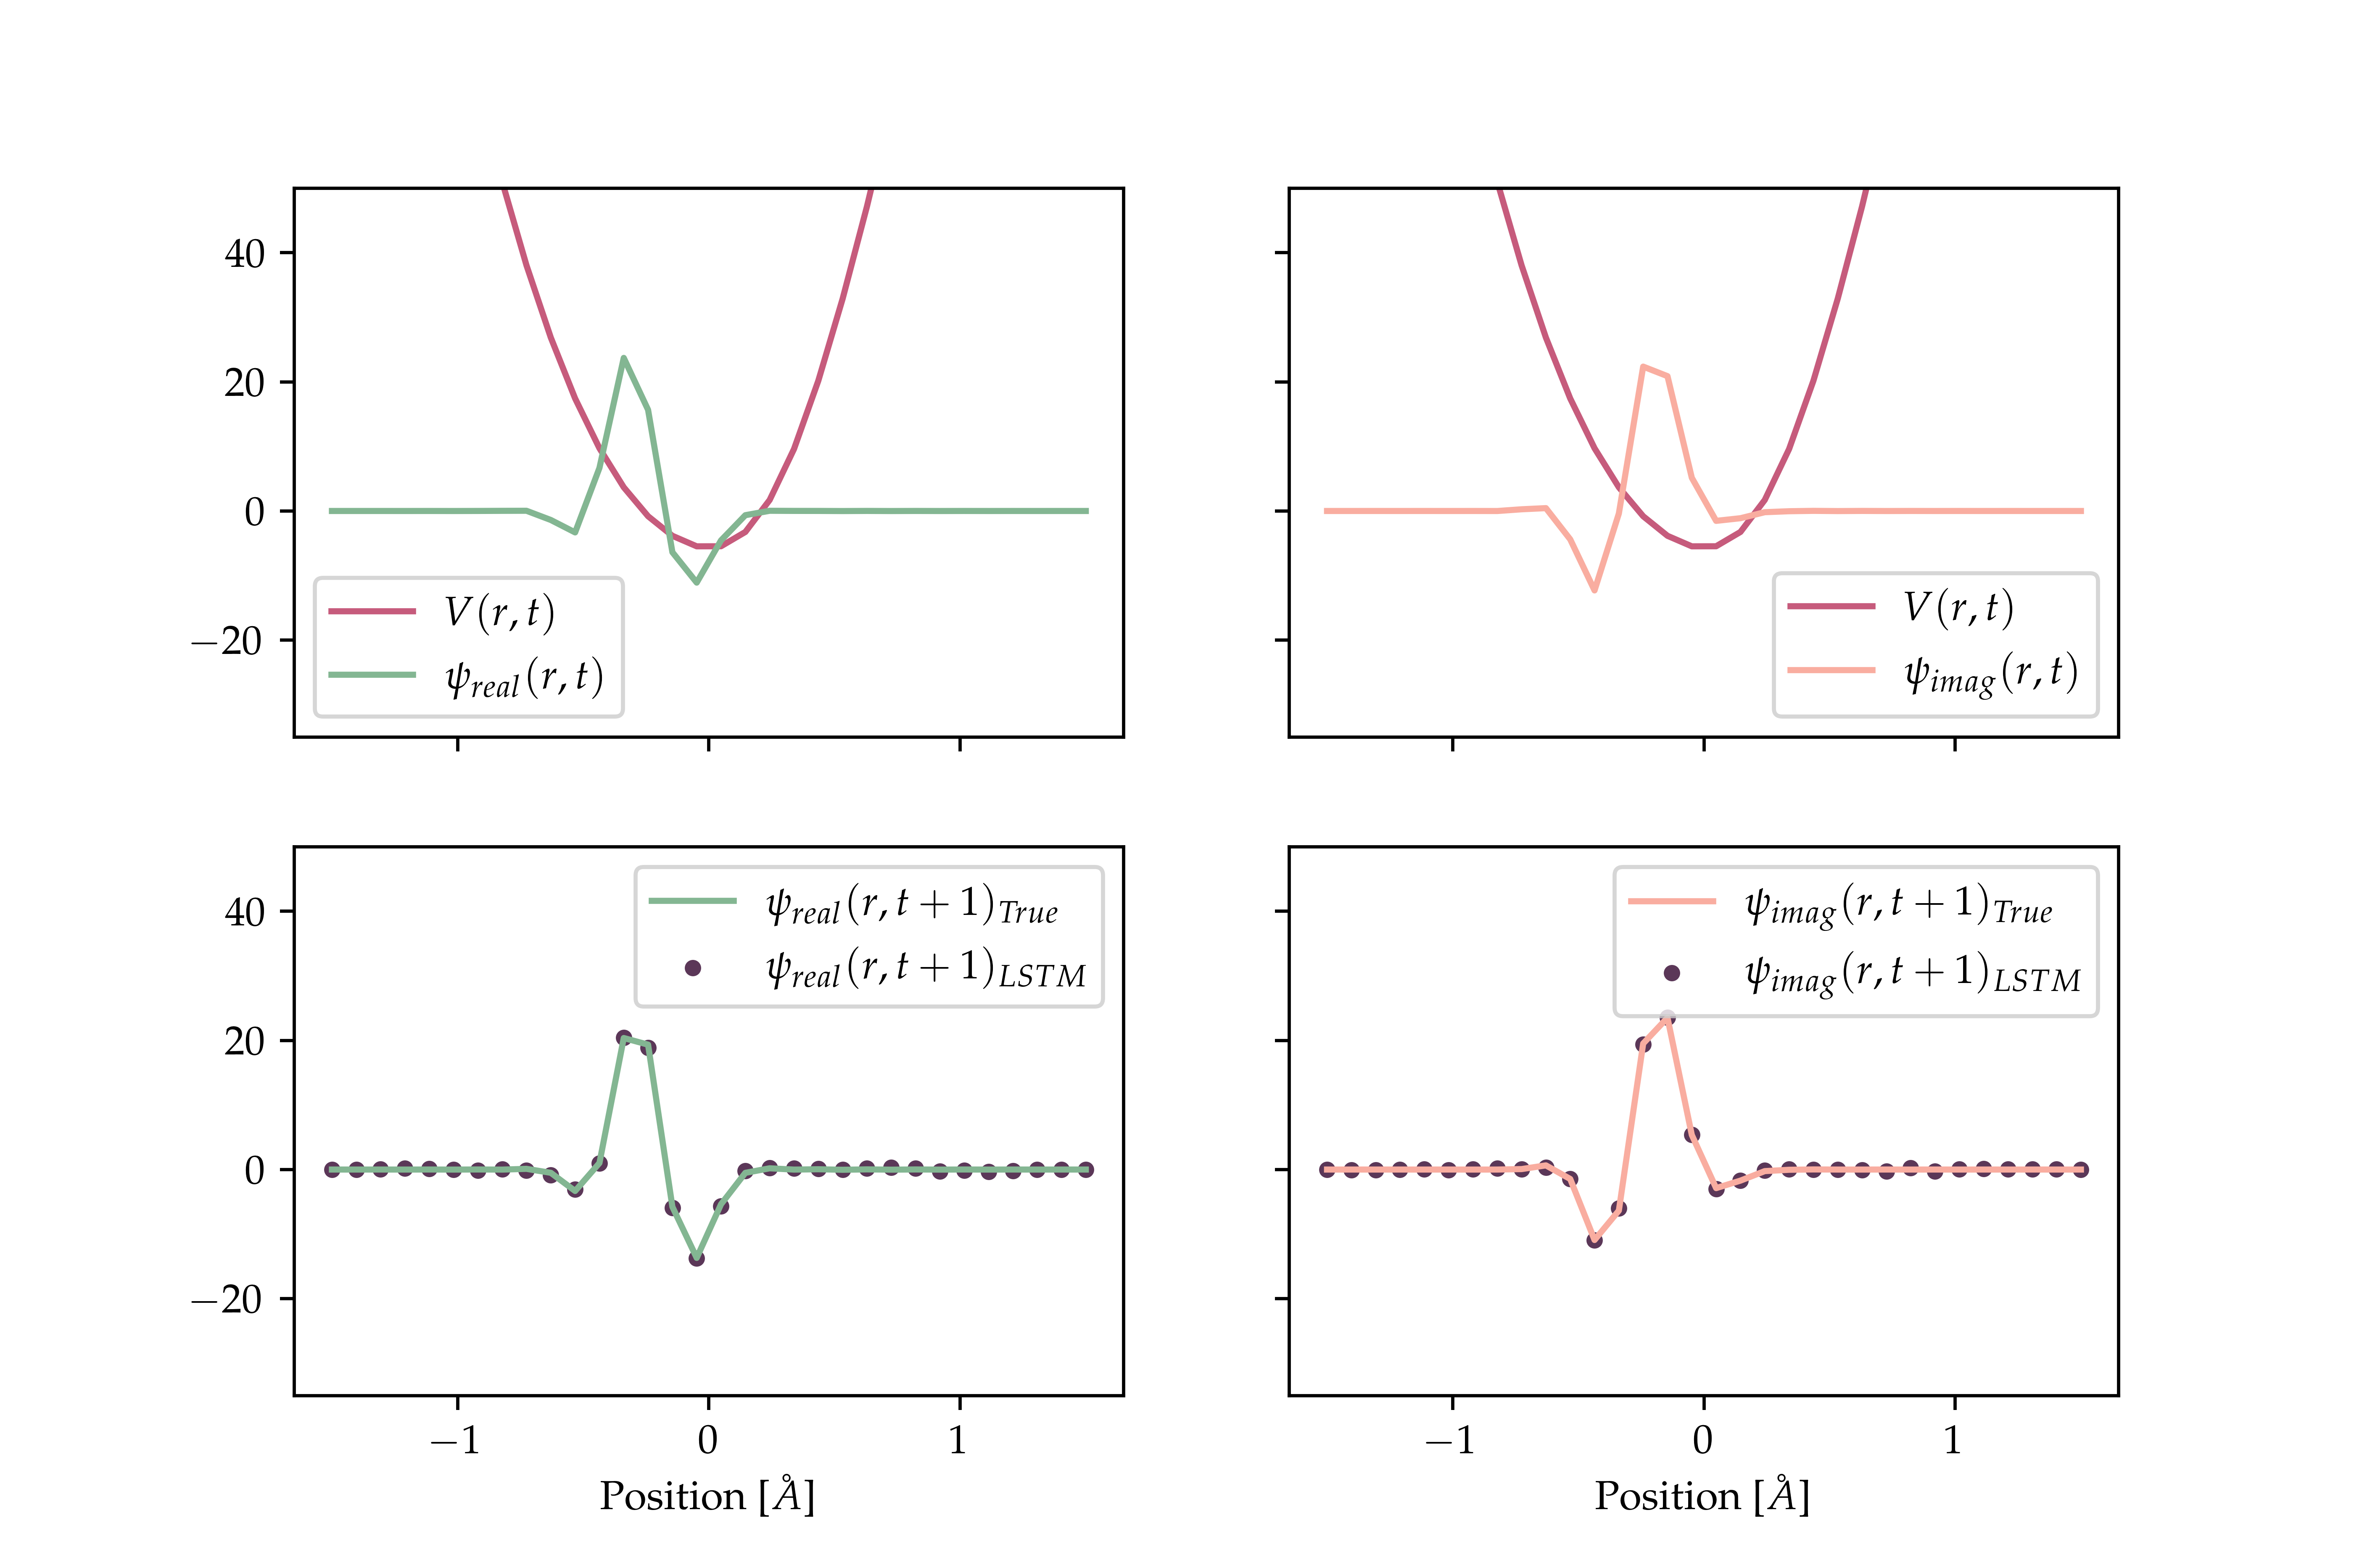
\includegraphics[width=1\textwidth]{/home/jessica/Tesis/img/tesis/model/1step.png}
  \caption{Predicción 1}
  \label{fig:1step}
\end{figure}

\begin{figure}[!htbp]
  \centering
  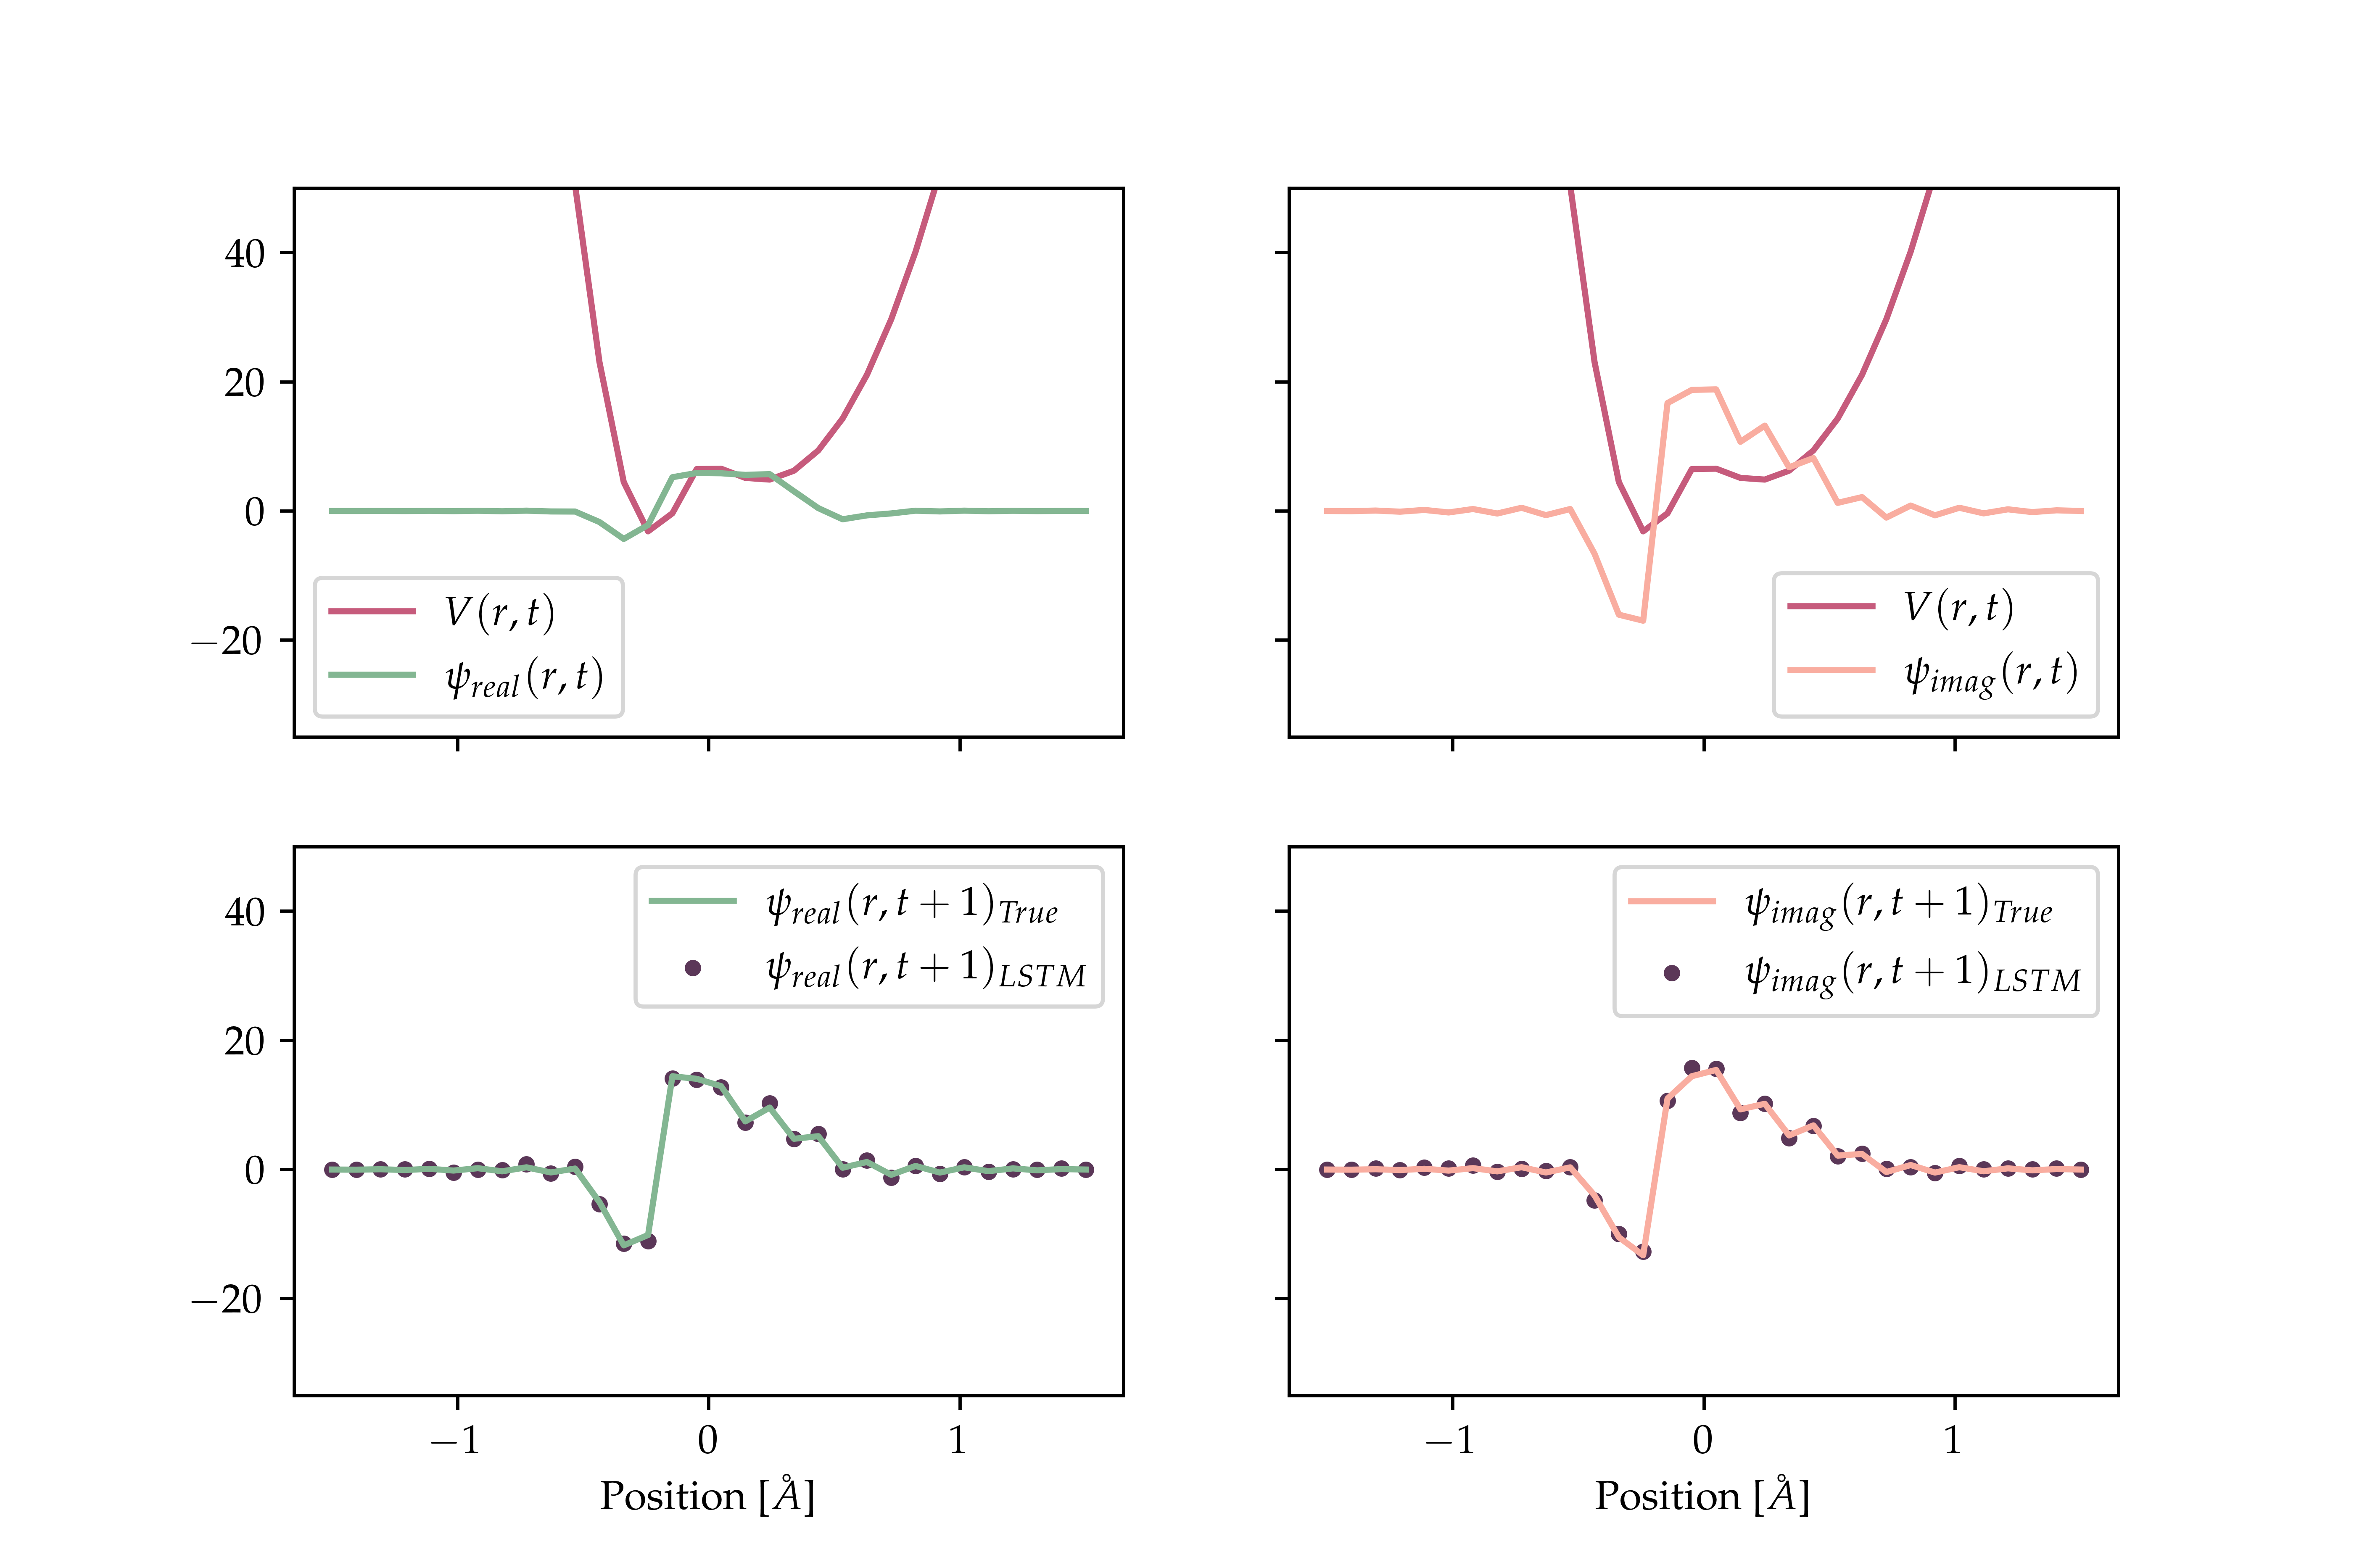
\includegraphics[width=1\textwidth]{/home/jessica/Tesis/img/tesis/model/1step1.png}
  \caption{Predicción 2}
  \label{fig:1step1}
\end{figure}

\begin{figure}[!htbp]
  \centering
  \includegraphics[width=1\textwidth]{/home/jessica/Tesis/img/tesis/model/trajDens.png}
  \caption{Trayectoria 1}
  \label{fig:trajec1}
\end{figure}

\begin{figure}[!htbp]
  \centering
  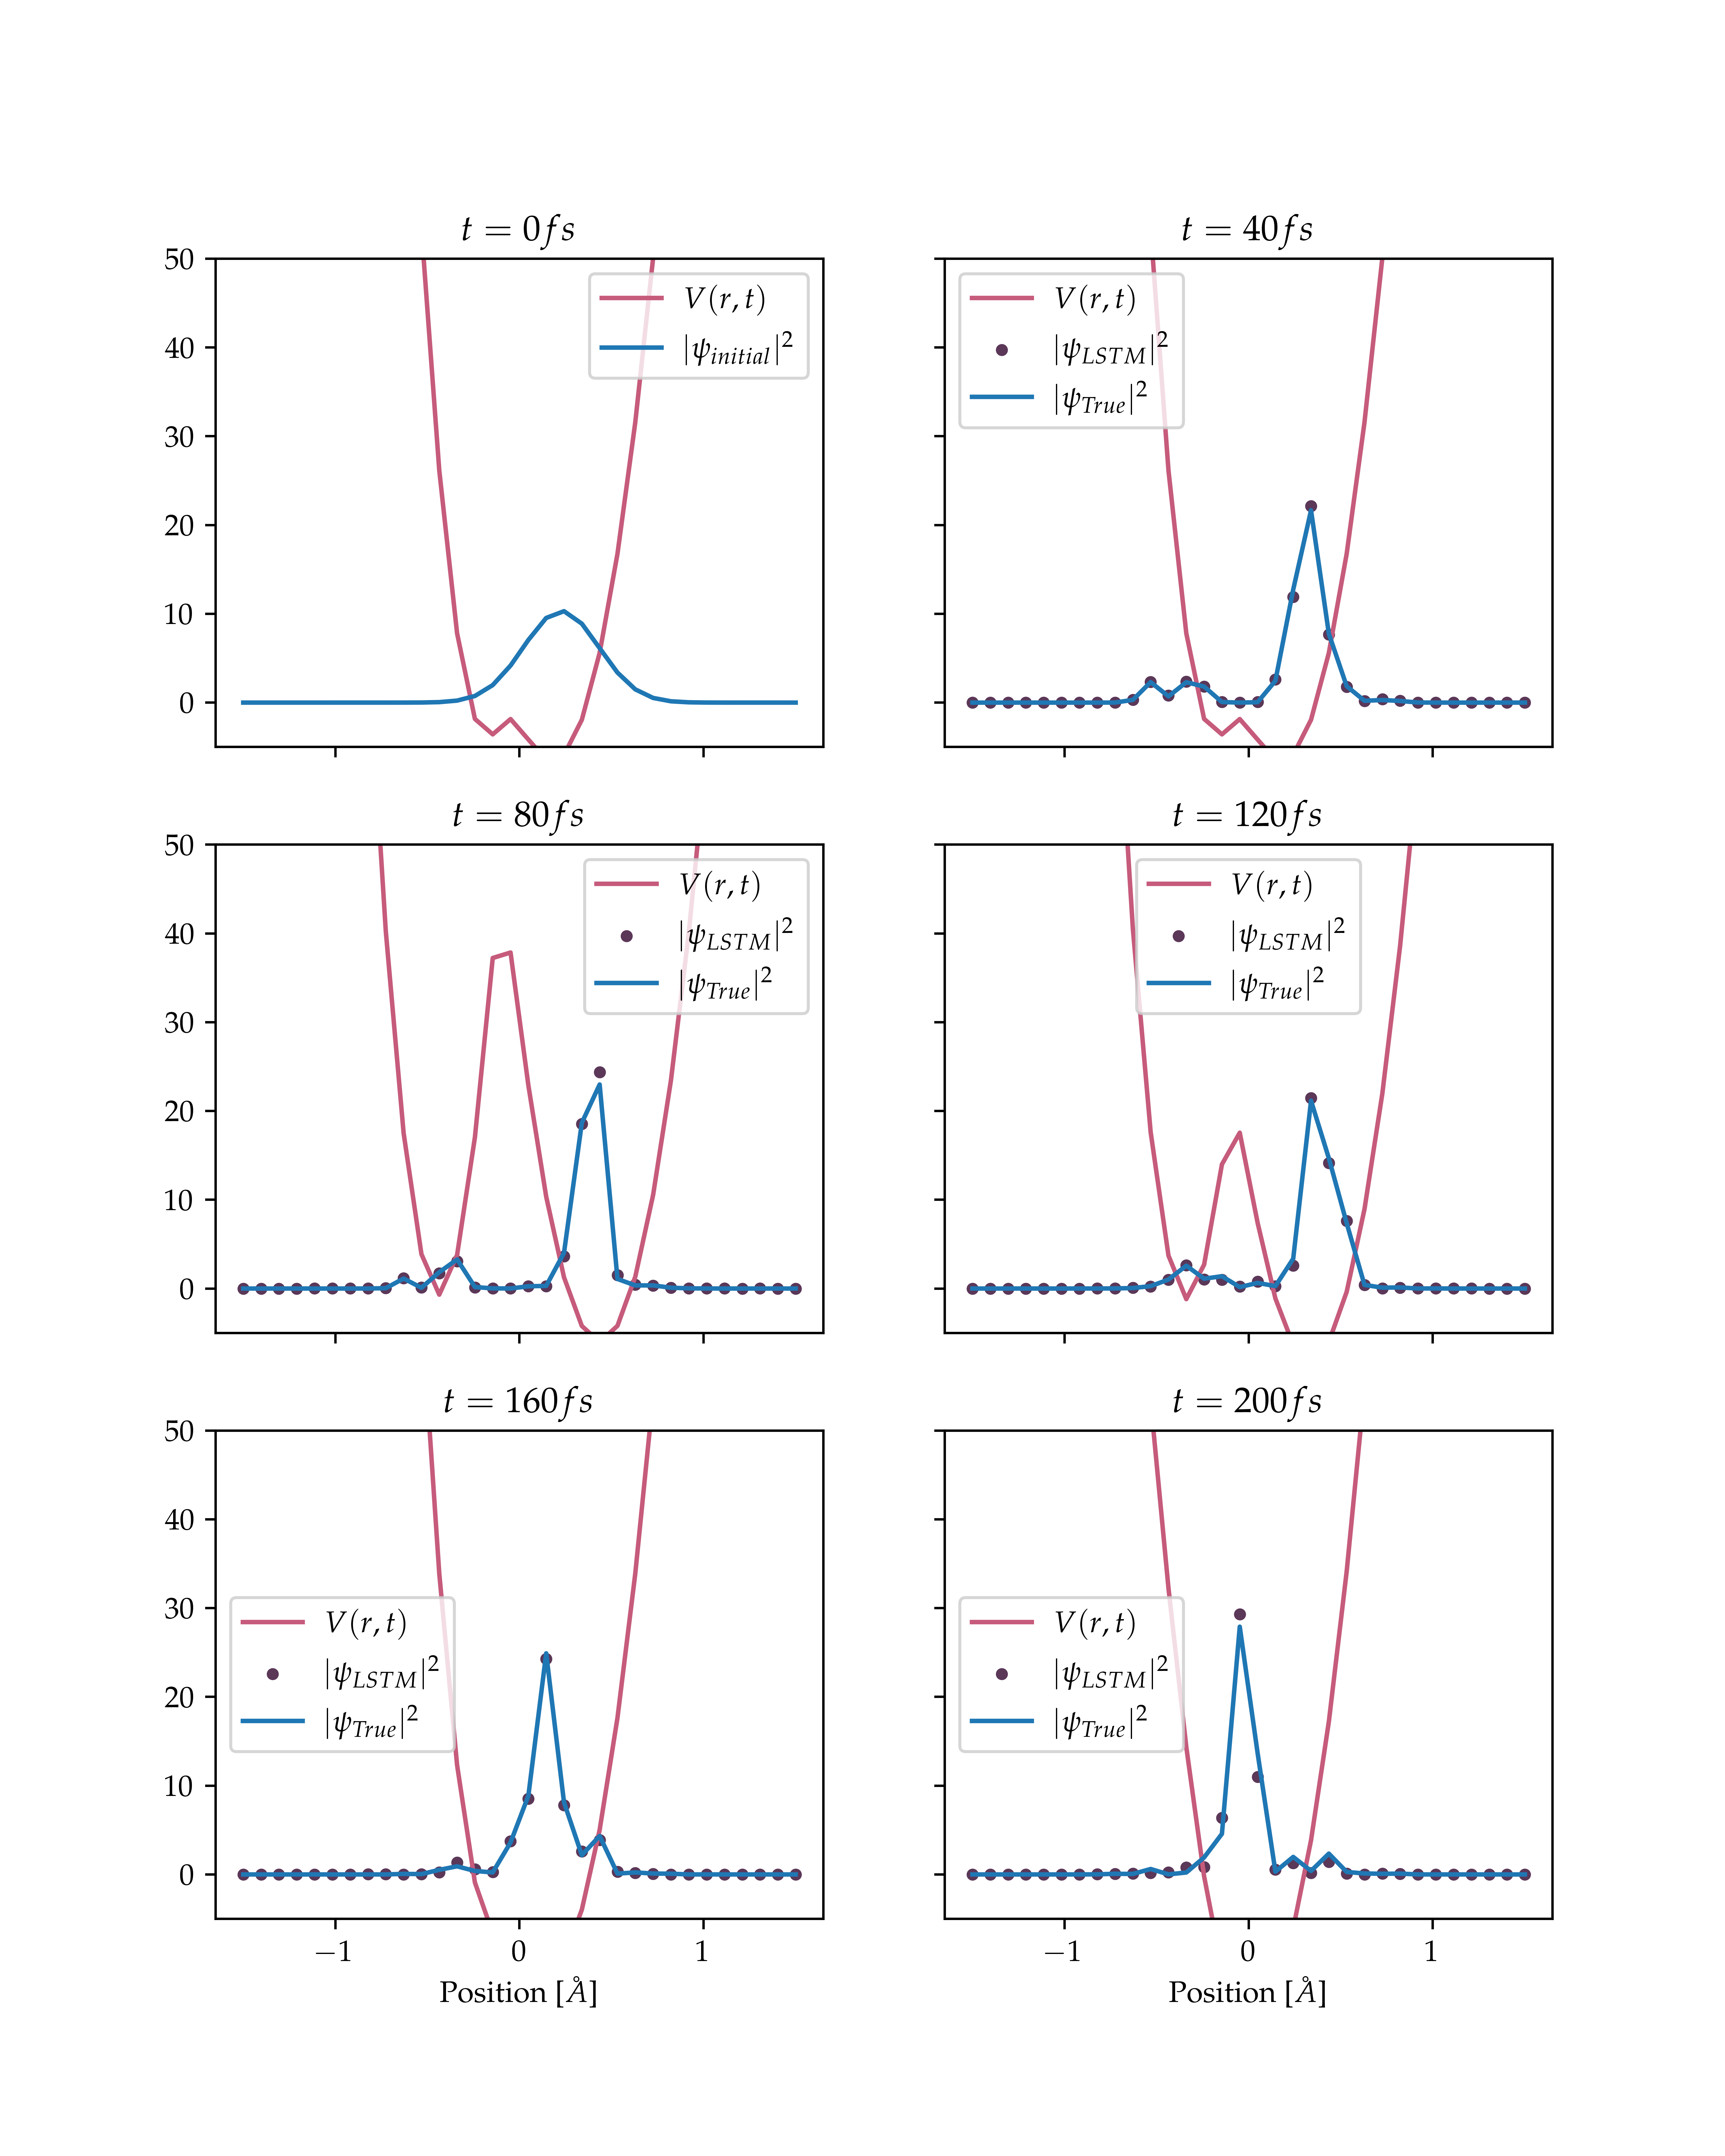
\includegraphics[width=1\textwidth]{/home/jessica/Tesis/img/tesis/model/trajDens1.png}
  \caption{Trayectoria 2}
  \label{fig:trajec2}
\end{figure}


\subsection{Análisis de Resultados}

\subsection{Conclusión}



%%************************************************
\chapter{Descripción del modelo}\label{ch:DescripModelo}
% ************************************************

% colocar aquí especificaciones técnicas, lenguaje de programación, framework utilizado,
% detalles de las versiones?

\section{Capas del la CNN}
% Sumary
% Diagrama ?


\section{Hiperparámetros y parámetros}
% epocas y lotes, así como tiempos de ejecución


%%************************************************
\chapter{Análisis de resultados y conclusión}\label{ch:ResultadosConclusion}
% ************************************************
\section{Presición del modelo}
% porcentaje o gráficas de costo/validacion

\section{Inferencias}

\section{Conclusión}

\subsection{Propuestas para mejorar el modelo}y




%\include{multiToC} % <--- just debug stuff, ignore for your documents
% ********************************************************************
% Backmatter
%*******************************************************
\appendix
%\renewcommand{\thechapter}{\alph{chapter}}
%agregar a forma final \cleardoublepage
\part{Apéndice}
%********************************************************************
% Appendix
%*******************************************************
% If problems with the headers: get headings in appendix etc. right
%\markboth{\spacedlowsmallcaps{Appendix}}{\spacedlowsmallcaps{Appendix}}
\chapter{Apéndice}
Lorem ipsum at nusquam appellantur his, ut eos erant homero
concludaturque. Albucius appellantur deterruisset id eam, vivendum
partiendo dissentiet ei ius. Vis melius facilisis ea, sea id convenire
referrentur, takimata adolescens ex duo. Ei harum argumentum per. Eam
vidit exerci appetere ad, ut vel zzril intellegam interpretaris.
\graffito{More dummy text.}



\section{Variables de Parámetros para el Potencial}
\begin{table}[h]
  \myfloatalign
  \begin{tabularx}{0.5\textwidth}{Xl} \toprule
   \tableheadline{Variable} & \tableheadline{Valor}\\ \midrule
    $V$          & 0.015936 $[a.u]$     \\ \midrule
    $\omega_1$   & 0.00811569 $[a.u]$   \\ \midrule
    $\omega_2$   & 0.00978836 $[a.u]$   \\ \midrule
    $\lambda$    & 0.00915455 $[a.u]$  \\ \midrule
    $X_{eq}$     & 0.00628338 $[a.u]$  \\ \midrule
    $\omega_x$   & 0.000357994 $[Jiffy^{-1}]$ \\ \midrule
    $\theta_X$   & 0.106646 $[rad]$   \\ \midrule
    $R_{eq}$     & 1.39712 $[a_0]$     \\ \midrule
    $R_0$        & 0.42091 $[a_0]$     \\ \midrule
    $\omega_{R}$ & 0.00135403 $[au]$   \\ \midrule
    $\theta_{R}$ & 4.52653 $[rad]$    \\ \midrule
    $m$          & 1836 $[m_e]$       \\
    \bottomrule
  \end{tabularx}
  \caption{Valores de parámetros del potencial utilizados para generar la gráfica de la \autoref{fig:drawPot}}
  \label{tab:ValuesPlot1}
\end{table}


\section{Unidades Atómicas}
\faHandshake[regular] No pelien

Equidem detraxit cu nam, vix eu delenit periculis. Eos ut vero
constituto, no vidit propriae complectitur sea. Diceret nonummy in
has, no qui eligendi recteque consetetur. Mel eu dictas suscipiantur,
et sed placerat oporteat. At ipsum electram mei, ad aeque atomorum
mea. There is also a useless Pascal listing below: \autoref{lst:useless}.

\begin{lstlisting}[float=b,language=Pascal,frame=tb,caption={A floating example (\texttt{listings} manual)},label=lst:useless]
for i:=maxint downto 0 do
begin
{ do nothing }
end;
\end{lstlisting}

%Ei solet nemore consectetuer nam. Ad eam porro impetus, te choro omnes
%evertitur mel. Molestie conclusionemque vel at, no qui omittam
%expetenda efficiendi. Eu quo nobis offendit, verterem scriptorem ne
%vix.



%********************************************************************
% Other Stuff in the Back
%*******************************************************
%agregar a forma final \cleardoublepage
%********************************************************************
% Bibliography
%*******************************************************
% work-around to have small caps also here in the headline
% https://tex.stackexchange.com/questions/188126/wrong-header-in-bibliography-classicthesis
% Thanks to Enrico Gregorio
%\defbibheading{bibintoc}[\bibname]{%
 % \phantomsection
  %\manualmark
  %\%markboth{\spacedlowsmallcaps{#1}}{\spacedlowsmallcaps{#1}}%
  %\addtocontents{toc}{\protect\vspace{\beforebibskip}}%
  %\addcontentsline{toc}{chapter}{\tocEntry{#1}}%
  %\chapter*{#1}%
  % }
\setquotestyle{english}
\printbibliography[heading=bibintoc]

% Old version, will be removed later
% work-around to have small caps also here in the headline
%\manualmark
%\markboth{\spacedlowsmallcaps{\bibname}}{\spacedlowsmallcaps{\bibname}} % work-around to have small caps also
%\phantomsection
%\refstepcounter{dummy}
%\addtocontents{toc}{\protect\vspace{\beforebibskip}} % to have the bib a bit from the rest in the toc
%\addcontentsline{toc}{chapter}{\tocEntry{\bibname}}
%\label{app:bibliography}
%\printbibliography

%\cleardoublepage%*******************************************************
% Declaration
%*******************************************************
\pdfbookmark[0]{Declaration}{declaration}
\chapter*{Declaration}
\thispagestyle{empty}
Put your declaration here.
\bigskip

\noindent\textit{\myLocation, \myTime}

\smallskip

\begin{flushright}
    \begin{tabular}{m{5cm}}
        \\ \hline
        \centering\myName \\
    \end{tabular}
\end{flushright}

%\cleardoublepage\pagestyle{empty}

\hfill

\vfill


\pdfbookmark[0]{Colophon}{colophon}
\section*{Colophon}
This document was typeset using the typographical look-and-feel \texttt{classicthesis} developed by Andr\'e Miede and Ivo Pletikosić.
The style was inspired by Robert Bringhurst's seminal book on typography ``\emph{The Elements of Typographic Style}''.
\texttt{classicthesis} is available for both \LaTeX\ and \mLyX:
\begin{center}
\url{https://bitbucket.org/amiede/classicthesis/}
\end{center}
Happy users of \texttt{classicthesis} usually send a real postcard to the author, a collection of postcards received so far is featured here:
\begin{center}
\url{http://postcards.miede.de/}
\end{center}
Thank you very much for your feedback and contribution.

\bigskip

\noindent\finalVersionString

%Hermann Zapf's \emph{Palatino} and \emph{Euler} type faces (Type~1 PostScript fonts \emph{URW
%Palladio L} and \emph{FPL}) are used. The ``typewriter'' text is typeset in \emph{Bera Mono},
%originally developed by Bitstream, Inc. as ``Bitstream Vera''. (Type~1 PostScript fonts were made
%available by Malte Rosenau and
%Ulrich Dirr.)

%\paragraph{note:} The custom size of the textblock was calculated
%using the directions given by Mr. Bringhurst (pages 26--29 and
%175/176). 10~pt Palatino needs  133.21~pt for the string
%``abcdefghijklmnopqrstuvwxyz''. This yields a good line length between
%24--26~pc (288--312~pt). Using a ``\emph{double square textblock}''
%with a 1:2 ratio this results in a textblock of 312:624~pt (which
%includes the headline in this design). A good alternative would be the
%``\emph{golden section textblock}'' with a ratio of 1:1.62, here
%312:505.44~pt. For comparison, \texttt{DIV9} of the \texttt{typearea}
%package results in a line length of 389~pt (32.4~pc), which is by far
%too long. However, this information will only be of interest for
%hardcore pseudo-typographers like me.%
%
%To make your own calculations, use the following commands and look up
%the corresponding lengths in the book:
%\begin{verbatim}
%    \settowidth{\abcd}{abcdefghijklmnopqrstuvwxyz}
%    \the\abcd\ % prints the value of the length
%\end{verbatim}
%Please see the file \texttt{classicthesis.sty} for some precalculated
%values for Palatino and Minion.
%
%    \settowidth{\abcd}{abcdefghijklmnopqrstuvwxyz}
%    \the\abcd\ % prints the value of the length

% ********************************************************************
% Game Over: Restore, Restart, or Quit?
% *******************************************************
%\printbibliography
\end{document}
% ********************************************************************
